%Copyrighted by Paulius Šarka, 2010. Some rights reserved.

\chapter{Skaičių teorija}
\thispagestyle{empty}

Skaičių teorija yra senas tradicijas turinti matematikos šaka, nagrinėjanti
uždavinius, susijusius su skaičiais ir jų dalumu. Šiame skyriuje
supažindinsime su pačiomis pagrindinėmis sąvokomis ir panagrinėsime dalelę
klasikinės teorijos -- liekanų grupes ir kvadratinius simbolius.

\section{Dalumas}

Su skaičių dalumo savoka jau greičiausiai esate pažįstami, tad pradžioje
keletas apibrėžimų pasitikslinimui. Turėkite omenyje, kad visur bus kalbama
apie natūraliuosius arba sveikuosius skaičius.

\begin{api} 
  Skaičius $n$ \emph{dalijasi} iš skaičiaus $a$, jei egzistuoja toks
  skaičius $b$, kad $n=a\cdot b$. Skaičius $a$ \emph{dalo} $n$ (žymėsime $a|n$)
  jei $n$ dalijasi iš $a$.  
\end{api}

\begin{api}
  Skaičius, iš kurio dalijasi $n$, vadinamas $n$ \emph{dalikliu}.
  Skaičius, kuris dalijasi iš $n$, vadinamas $n$ \emph{kartotiniu}.  
\end{api}

\begin{api} 
  Skaičius, kuris dalijasi tik iš vieneto ir iš savęs, vadinamas
  \emph{pirminiu}. 
\end{api}

Sveikųjų skaičių dalyba tenkina keletą savybių. Įsitikinkite, kad
suprantate kiekvieną, ir mintyse pabandykite sugalvoti po pavyzdį:

\begin{itemize} 
  \item Jei $x|a$ ir $x|b$, tai $x|a+b$, $x|a-b$ ir $x|ab$;
  \item Jei $x|y$ ir $y|z$, tai $x|z$; 
  \item Jei $x|a$ ir $y|b$, tai $xy|ab$.  
  %\item Jei $x|a_1 + a_2 + \cdots + a_n$, $x|a_1, x|a_2, \dots,
  %x|a_{n-1}$, tai $x|a_n$.  
\end{itemize}

\subsubsection{Skaidymas dauginamaisiais}
Viena iš pagrindinių sveikųjų skaičių savybių, susijusių su dalumu, yra
vienareikšmis skaidymasis dauginamaisiais. Ja mes remsimės ir naudosimės
labai dažnai, nors jos ir neįrodysime (įrodymas yra kiek ilgokas ir vargu,
ar tinkamas pačiai pažinties su skaičių teorija pradžiai).

\begin{teig} 
  Kiekvieną skaičių $n$ galima vieninteliu būdu išskaidyti
  pirminiais dauginamaisiais: $$n=p_1^{\alpha_1}p_2^{\alpha_2}\cdots
  p_k^{\alpha_k}.$$ 
\end{teig}

Mažus skaičius skaidyti pirminiais dauginamaisiais nesunku -- tiesiog iš eilės tikriname
pirminius skaičius ir skaičiuojame, kiek kartų iš jų galima padalinti.
Pavyzdžiui, $$120 = 2\cdot 2 \cdot 2 \cdot 3 \cdot 5 = 2^3\cdot 3 \cdot 5.$$

Žinodami, kaip skaičius išsiskaido, galime nemažai apie jį pasakyti.
Pavyzdžiui, galime nurodyti jo daliklius:

\begin{teig} Jei skaičius $n$ dalijasi iš skaičiaus $a$ ir
  $$n=p_1^{\alpha_1}p_2^{\alpha_2}\cdots p_k^{\alpha_k},$$ tai tuomet
  $$a=p_1^{\beta_1}p_2^{\beta_2}\cdots p_k^{\beta_k}$$ ir $$\beta_i \leq
  \alpha_i$$ su visais $i=1,\dots,k$.  
\end{teig}

\begin{proof}[Įrodymas] Jei $n$ dalijasi iš $a$, tai tuomet egzistuoja toks $b$,
  kad $n=ab$. Išskaidę $a$ dauginamaisiais gauname, kad į $n$ skaidinį turi 
  įeiti visi pirminiai kaip ir į $a$ su nemažesniais laipsnių rodikliais.
\end{proof}

Panagrinėkime skaičių $12$. Jis išsiskaido kaip $2^2\cdot 3^1$. Pagal ką
tik įrodytą teiginį jo dalikliais turėtų būti $2^2 \cdot 3^1$,$2^1 \cdot
3^1$, $2^0 \cdot 3^1$, $2^2 \cdot 3^0$, $2^1 \cdot 3^0$ ir $2^0 \cdot 3^0$.
Sudauginę matome, kad gavome skaičius $12$, $6$, $3$, $4$, $2$ ir $1$,
kurie iš ties yra visi $12$ dalikliai. 
Tad norėdami rasti duoto skaičiaus daliklį turime paimti kažkokią dalį jo
skaidinio. Šis pastebėjimas leidžia nesunkiai suskaičiuoti, kiek iš viso
daliklių skaičius turi:

\begin{teig} Skaičius $n = p_1^{\alpha_1}p_2^{\alpha_2}\cdots
  p_k^{\alpha_k}$ turi $(\alpha_1 + 1)(\alpha_2 + 1)\cdots (\alpha_n + 1)$
  daliklių.  
\end{teig}

\begin{proof}[Įrodymas] Kiekvienas $n$ daliklis bus užrašomas kaip
  $p_1^{\beta_1}p_2^{\beta_2}\cdots p_k^{\beta_k}$, kur $\beta_i \leq
  \alpha_i$ su visais $i=1,\dots,k$. Skirtingus daliklius gausime imdami
  skirtingus pirminių skaičių laipsnius. Parinkti $\beta_1$ galime $\alpha_1
  + 1$ būdais (nepamirškime nulio!), parinkti $\beta_2$ galime $\alpha_2 + 1$
  būdais ir taip toliau. Pagal kombinatorinę daugybos taisyklę iš viso
  galėsime sudaryti $(\alpha_1 + 1)(\alpha_2 + 1)\cdots (\alpha_n + 1)$
  skirtingų laipsnių rinkinių, todėl tiek bus ir skirtingų daliklių.
\end{proof}

\subsubsection{Didžiausiasis bendras daliklis}

Prisiminkime didžiausiojo bendro daliklio ir mažiausiojo bendro kartotinio
sąvokas.

\begin{api}Dviejų ar daugiau skaičių \emph{didžiausiuoju bendru dalikliu} ($\dbd$)
  vadinsime didžiausią skaičių, iš kurio visi duotieji dalinasi.  
\end{api}

\begin{api} Dviejų ar daugiau skaičių \emph{mažiausiuoju bendru kartotiniu} ($\mbk$)
  vadinsime mažiausią skaičių, kuris dalijasi iš visų duotųjų.  
\end{api}

\begin{api}
  Du skaičius, kurių didžiausiasis bendras daliklis yra lygus $1$, vadinsime
  \emph{tarpusavyje pirminiais}.
\end{api}

Pavyzdžiui, didžiausias skaičius, iš kurio dalijasi ir $15$ ir $25$, yra $5$,
o mažiausias skaičius, kuris dalijasi iš $2$, $3$, $4$, $5$ ir $6$, yra
$60$. Tad $\dbd(15,25)=5$ ir $\mbk(2,3,4,5,6)=60$. Ieškant didžiausiojo
bendro daliklio ir mažiausiojo bendro kartotinio labai praverčia skaidymas
dauginamaisiais. Įsižiūrėkite:

Norėdami rasti didžiausią skaičių $2^4\cdot3^1$ ir $2^1\cdot3^1\cdot5^1$
bendrą daliklį turime paimti didžiausią įmanomą skaidinio dalį,
priklausančią abiems skaičiams. Šiuo atveju tai būtų $2^1\cdot3^1$.

Norėdami rasti mažiausią skaičių $2^4\cdot3^1$ ir $2^1\cdot3^1\cdot5^1$
bendrą kartotinį, turime paimti mažiausią įmanomą skaidinį, į kurį "tilptų"
abiejų skaičių skaidiniai. Šiuo atveju tai būtų $2^4 \cdot 3^1 \cdot 5^1$.

Kitas būdas, ar bent jau pagrindinė idėja, kuri praverčia ieškant
didžiausio bendro daliklio, yra Euklido algoritmas. Jis remiasi svarbia ir
naudinga lygybe:
\begin{teig}
  $$\dbd(a,b) = \dbd(a-b,b).$$
\end{teig}

\begin{proof}[Įrodymas]
Tegu $\dbd(a,b)=d$. Tuomet $d|a$ ir $d|b$, o kartu $d|(a-b)$. Vadinasi,
$\dbd(a-b,b)$ bus nemažesnis nei $d$.  

Iš kitos pusės -- tegu $\dbd(a-b,b) = d'$. Kartut $d'|(a-b)$ ir $d'|b$, o
tuo pačiu $d'|a$, nes $a = (a-b) + b$.  Vadinasi, $\dbd(a,b)$ bus nemažesnis
nei $d'$. 

Kadangi gavome $d\geq d'$ ir $d' \geq d$, tai vadinasi $d=d'$, t.y.
$\dbd(a,b) = \dbd(a-b,b)$.
\end{proof}

\begin{pav}
  Pasinaudodami įrodyta lygybe raskime $\dbd(14,6)$,
  $\dbd(2^{100}+1, 2^{100}-1)$ ir $\dbd( (p+q)^2, p)$, kur $p$ ir
  $q$ pirminiai skaičiai. 
\end{pav}

\begin{sprendimas}
Didžiausio bendro daliklio ieškosime atimdami iš didesnio skaičiaus
mažesnį:
$$\dbd(14,6) = \dbd(8,6) = \dbd(2,6) = \dbd(2,4) = \dbd(2,2)= 2.$$
$$\dbd(2^{100} + 1, 2^{100} - 1) = \dbd(2,2^{100}-1) = 1.$$
$$\dbd( (p+q)^2, p) = \dbd(p(p + 2q) + q^2, p) = \dbd(q^2 , p) = 1.$$
\end{sprendimas}

\theoremstyle{plain}\newtheorem*{euklidoalg}{Euklido algoritmas}
\begin{euklidoalg} Rasime $\dbd(a,b)$. Nemažindami bendrumo tarkime, kad $a > b$. Tuomet $a$
užrašomas kaip \\
$a = bq + r$, kur dalybos liekana tenkina $0 < r < b$. Analogiškai \\
$b = rq_{1} + r_{1}$, kur $0 < r_{1} < r$, \\
$r = r_{1}q_{2} + r_{2}$, kur $0 < r_{2} < r_{1}$, \\
$\hdots$ \\
$r_{k-2} = r_{k-1}q_{k} + r_{k}$, kur $0 < r_{k} < r_{k-1}$,
\\
$r_{k-1} = r_{k}q_{k+1}.$ \\

Iš $r > r_{1} > ... > r_{k}$ seka, kad kažkada gausime dalybos liekaną
lygią $0$. Tuomet, kadangi $$\dbd(a,b) = \dbd(b,r) = \cdots =
\dbd(r_{k-2},r_{k-1}) = \dbd(r_{k-1},r_{k}),$$ tai paskutinioji nenulinė
liekana $r_{k}$ ir bus didžiausias bendrasis daliklis.
\end{euklidoalg}

Paties Euklido algoritmo taip skrupulingai, kaip jis suformuluotas,
netaikysime -- dažniausiai, kaip pavyzdyje, pakaks keletą kartų pasinaudoti
lygybe $\dbd(a,b) = \dbd(a, b-a)$. Tačiau užrašėme jį ne be reikalo -- labai
svarbi bus jo išvada:

\begin{isv} 
  Jei $\dbd(a,b)=d$, tai egzistuoja tokie $x,y \in \Z$, kad $ax + by = d$.
\end{isv}

\begin{proof}
  Iš priešpaskutinės Euklido algoritmo lygybės galime išreikšti $r_{k}$ per
  $r_{k-1}$ ir $r_{k-2}$. Iš dar ankstesnės galima išreikšti $r_{k-1}$ per
  $r_{k-2}$ ir $r_{k−3}$. Įstatę į pirmąją išraišką gausime $r_{k}$ išraišką
  per $r_{k-2}$ ir $r_{k−3}$. Taip toliau vis tęsdami gausime $r_{k}$ išraišką
  per $a$, $b$, t.y. rasime $x$, $y$, tenkinančius $ax + by = \dbd(a,b).$
\end{proof}

\subsubsection{Pirminiai skaičiai}

Jau pirmuosiuose puslapiuose galima atkreiptį dėmesį į tai, kokį didelį vaidmenį
skaičių teorijoje vaidina pirminiai skaičiai. Kadangi kiekvieną sveikąjį
skaičių vieninteliu būdu galima užrašyti kaip jų sandaugą, tai neretai jie
yra vaizdžiai vadinami sveikųjų skaičių atomais. Įrodykime vieną iš
gražiausių ir elegantiškiausių matematikos teoremų:

\begin{thm} 
  Pirminių skaičių yra be galo daug.  
\end{thm} 

\begin{proof} 
  Tarkime priešingai, kad pirminių skaičių yra baigtinis skaičius.
  Sudauginkime juos visus ir pridėkime vienetą: $p_1p_2\cdots p_n + 1$. Šis
  skaičius nesidalija iš nė vieno pirminio $p_1, \dots, p_n,$ todėl pats
  yra pirminis. Gavome naują pirminį -- prieštara.
\end{proof}

Kartais tenka patikrinti, ar duotas skaičius yra pirminis, ar ne. Tam reikia
patikrinti visus potencialius jo daliklius. Truputį pagalvoję, galime rasti
sutrumpinimą: 

\begin{teig} 
  Jei skaičius $n$ nesidalija iš jokio pirminio skaičiaus, mažesnio (arba
  lygaus) už $\sqrt{n}$, tai jis pirminis.
\end{teig} 

\begin{proof}
  Išties, jei skaičius $n$ turi daliklį $a$, tai turi ir daliklį
  $\frac{n}{a}$, bet tuomet arba $a\leq \sqrt{n}$, arba $\frac{a}{n} \leq
  \sqrt{n}$, vadinas,i $n$ turės daliklį (o kartu ir pirminį daliklį),
  mažesnį už $\sqrt{n}$. 
\end{proof}

Pavyzdžiui, norint patikrinti, ar $101$ yra pirminis, užtenka išbandyti $2$,
$3$, $5$ ir $7$. Kadangi nė iš vieno nesidalija, tai 101 yra pirminis.

\subsubsection{Dalumo požymiai}

Užrašę skaičių dešimtainėje sistemoje $\overline{a_1a_2\dots a_n}$, iš jo
skaitmenų galime spręsti, ar jis dalijasi iš kai kurių mažų skaičių, ar ne.
Naudingiausi dalumo požymiai yra šie:

\begin{itemize} 
  \item Skaičius $\overline{a_1a_2\dots a_n}$ dalijasi iš $2$, jei iš $2$
    dalijasi jo paskutinis skaitmuo $a_n$.  
  \item Skaičius $\overline{a_1a_2\dots a_n}$ dalijasi iš $3$, jei iš $3$
    dalijasi jo skaitmenų suma $a_1 + \cdots + a_n$.  
  \item Skaičius $\overline{a_1a_2\dots a_n}$ dalijasi iš $4$, jei iš $4$
    dalijasi jo dviejų skaitmenų galūnė $\overline{a_{n-1}a_n}$.  
  \item Skaičius $\overline{a_1a_2\dots a_n}$ dalijasi iš $5$, jei iš $5$
    dalijasi jo paskutinis skaitmuo $a_n$.  
  \item Skaičius $\overline{a_1a_2\dots a_n}$ dalijasi iš $8$, jei iš $8$
    dalijasi jo trijų skaitmenų galūnė $\overline{a_{n-2}a_{n-1}a_n}$.  
  \item Skaičius $\overline{a_1a_2\dots a_n}$ dalijasi iš $9$, jei iš $9$
    dalijasi jo skaitmenų suma $a_1 + \cdots + a_n$.  
  \item Skaičius $\overline{a_1a_2\dots a_n}$ dalijasi iš $11$, jei iš $11$
    dalijasi jo alternuojanti skaitmenų suma $a_1 -a_2+a_3-a_4+ \cdots \pm
    a_n$.  
\end{itemize}

Visų dalumo požymių įrodymai bus išmėtyti po pirmus du skyrelius, o kol kas
svarbiau juos įsiminti ir išmokti atpažinti.

\subsubsection{Pavyzdžiai}

\begin{pavnr} Įrodykite, kad su visais natūraliaisiais $n$, $n^2 + n$
  dalijasi iš $2$.  
\end{pavnr}

\begin{sprendimas}
  Jei $n$ dalijasi iš $2$, tai ir $n^2$ dalijasi iš dviejų. Dviejų skaičių,
  besidalijančių iš dviejų (lyginių), suma taip pat dalinsis iš dviejų.

  Jei $n$ nesidalija iš $2$, tai ir $n^2$ nesidalija iš dviejų. Dviejų
  skaičių, nesidalijančių iš dviejų (nelyginių) suma dalijasi iš dviejų. 

  Vadinasi, tikrai, bet kuriuo atveju, $n^2 + n$ dalinsis iš dviejų.
\end{sprendimas}

\begin{pavnr} 
  Įrodykite, kad jei $n|5a + 3b$ ir $n|3a+2b$, tai $n|a$ ir $n|b$.
\end{pavnr}

\begin{sprendimas}
Pastebėkime, kad $a$ galime išreikšti kaip $2(5a+3b)-3(3a+2b)$, o $b$ kaip
$5(3a+2b)-3(5a+3b)$. Abu skirtumai iš $n$ dalijasi, todėl dalinsis ir $a$,
ir $b$. 
\end{sprendimas}

\begin{pavnr}
  Įrašykite žvaigždučių vietoje tokius skaitmenis, kad skaičius $15**15$
  dalytųsi iš $99$.  
\end{pavnr}

\begin{sprendimas}
  Duotas skaičius dalinsis iš $99$ tada ir tik tada, kai dalinsis iš
  $9$ ir iš $11$. Jei vietoje žvaigždučių įrašysime $x$ ir $y$, tai pagal dalumo
  požymius gausime, kad $12+x+y$ turi dalintis iš $9$, ir $x-y-8$ turi
  dalintis iš $11$. Abi sąlygas tenkina $x=6$, $y=9$.
\end{sprendimas}

\begin{pastaba}
  Teiginys, kad $n$ dalinasi iš $ab$ tada ir tik tada, kai $n$ dalinasi iš
  $a$ ir $n$ dalinasi iš $b$, yra teisingas, tik kai $a$ ir $b$ yra
  tarpusavyje pirminiai.  
\end{pastaba}


\begin{pavnr}
  Įrodykite dalumo iš $3$ požymį. 
\end{pavnr}

\begin{sprendimas}
Skaičius, užrašytas dešimtaine išraiška kaip $\overline{a_1a_2\dots a_n}$,
yra lygus $a_1\cdot 10^{n-1} + a_2\cdot 10^{n-2} + \cdots + a_{n-1}\cdot 10 + a_n$.
Pastebėkime, kad visi dešimties laipsniai yra vienetu didesni už skaičių,
besidalijantį iš trijų:
\begin{align*}
  & a_1 \cdot 10^{n-1} + a_2  \cdot10^{n-2} + \cdots + a_{n-1} \cdot 10 + a_n = \\
  & a_1 \cdot \underbrace{99\dots 9}_{n-1} + a_2 \cdot \underbrace{99\dots 9}_{n-2} + \cdots
  + a_{n-1} \cdot 9 + a_1 + a_2 + \cdots + a_{n-1} + a_n.
\end{align*}
Matome, kad skaičius nuo savo skaitmenų sumos skiriasi per $3$ kartotinį,
todėl arba abu dalijasi iš trijų, arba abu nesidalija. 
\end{sprendimas}

\begin{pavnr}\text{\emph{[IMO 1959]}} Įrodykite, kad trupmena $\frac{21n+4}{14n+3}$ yra
  nesuprastinama su visomis natūraliosiomis $n$ reikšmėmis.
\end{pavnr}

\begin{sprendimas}
  Trupmena bus nesuprastinama, jei didžiausias skaitiklio ir vardiklio
  bendras daliklis bus lygus vienam. Pasinaudoję $\dbd(a,b) = \dbd(a, b-a)$
  gauname: $$\dbd(21n + 4, 14n + 3) = \dbd(7n+1, 14n+3) = \dbd(7n+1,1) =
  1.$$
\end{sprendimas}


\subsubsection{Uždaviniai}

\begin{enumerate} 
  \item Duota, kad $n|3a$ ir $n|12a+5b$. Įrodykite, kad $n|10b$.  
    %Jei $n|3a$, tai $n|12a$ ir $n|12a + 5b - 12a = 5b$. Aišku, kad iš
    %$n|5b$ seka ir $n|10b$.
  \item Duota, kad $n|3a + 7b$ ir $n|2a+5b$.  Įrodykite, kad $n|a$ ir $n|b$.  
    %Pastebėkime, kad $b$ galima išreikšti kaip $3(2a+5b) - 2(3a+7b)$, o
    %$a$ kaip $5(3a+7b) - 7(2a+5b)$, vadinasi, abu jie iš $n$ dalinsis.
  \item Ar teisingos šios "dalumo savybės": 

    a) Jei $x|a + b$, tai $x|a$ ir $x|b$,

    b) Jei $x|a\cdot b$, tai $x|a$ arba $x|b$,

    c) Jei $x|a$ ir $y|a$, tai $xy|a$ ?
    %Ne, jos visos trys neteisingos.
    %
    %a) Jei $x|a+b$, tai nebūtinai $x|a$ ir $x|b$. Pavyzdžiui, $5|2+3$, bet
    %$5\nmid 2$ ir $5\nmid 3$.
    %
    %b) Jei $x|a\cdot b$, tai nebūtinai $x|a$ arba $x|b$. Pavyzdžiui,
    %$6|2\cdot 3$, bet $6\nmid 2$ ir $6\nmid 3$. Kaip bebūtų, ši savybė
    %teisinga, kai $x$ pirminis (jei dviejų skaičių sandauga dalijasi iš
    %pirminio skaičiaus, tai iš to pirminio dalijasi nors vienas iš
    %skaičių).
    %
    %c) Jei $x|a$ ir $y|a$, tai nebūtinai $xy|a$. Pavyzdžiui, $4|12$ ir
    %$6|12$, bet $24\nmid 12$.
  \item Įrodykite, kad bet kaip sudėliojus devynis skaitmenis
    $1$, $2$,..., $9$, gautas devynženklis skaičius dalinsis iš $9$.  
    %Taip gauto skaičiaus skaitmenų suma yra lygi $45$, tad pagal dalumo
    %požymį jis iš $9$ dalinsis.
  \item Įrodykite, kad skaičius $\overline{abba}$ dalijasi iš $11$.  
    %Pritaikome dalybos iš $11$ požymį: $a-b +b-a =0$ dalijasi iš
    %$11$, vadinasi ir skaičius $\overline{abba}$ dalinsis iš $11$.
  \item Įrašykite žvaigždutes vietoje tokį skaitmenį, kad skaičius $12345*$
    dalytųsi iš: a) $9$; b) $8$; c) $11$.  
    %a) Jei vietoje žvaigždutės įrašysime $x$, tai gauto skaičiaus
    %skaitmenų suma bus lygi $15+x$. Ji dalinsis iš $9$ kai $x=3$
    %
    %b) Pagal dalumo požymį iš $8$ turi dalintis $45*$. Kadangi $400$
    %dalijasi iš $8$ ir $56$ dalijasi iš $8$ tai vietoje žvaigždutės galime
    %įrašyti $6$.
    %
    %c) Alternuojanti suma vietoj žvaigždutės įrašius $x$ yra lygi
    %$3-x$. Ji dalinsis iš $11$, kai $x=3$.
  \item Duota, kad skaičius $a+4b$ dalijasi iš $13$. Įrodykite, kad ir
    $10a+b$ dalijasi iš $13$. 
    %Pakanka pastebėti, kad $10a+b$ yra lygus $10(a+4b) -13\cdot 3b$.
 \item Raskite visus pirminius skaičius iš intervalo $[180, 200]$.  
    %Atmetę lyginius ir dalius iš $5$ skaičius gauname, kad lieka
    %patikrinti $181$, $183$, $187$, $189$, $191$, $193$, $197$ ir $199$. Pagal dalumo
    %požymius $183$ ir $189$ dalijasi iš $3$, o $187$ iš $11$. Iš
    %$7$ šitame intervale dalijasi skaičiai $182, 189$ ir $196$, o iš
    %$13$ tik $182$. Vadinasi, skaičiai $181, 191, 193, 197$ ir $199$
    %nesidalija iš pirminių, mažesnių už $\sqrt{199} \approx 14$, todėl
    %yra pirminiai.
  \item Su kuriomis natūraliosiomis $n$ reikšmėmis skaičius $n^2 + 5n + 6$
    pirminis?  
    %Išskaidykime: $n^2 + 5n + 6 = (n+2)(n+3)$. Kadangi su visomis
    %natūraliosiomis $n$ reikšmėmis abu dauginamieji yra didesni už
    %$1$, tai jų sandauga niekada nebus pirminis skaičius.
  \item Duota, kad $n|a+b$. Įrodykite, kad $n|a^3+2a+b^3+2b$.  
    %Išskaidykime dauginamaisiais: $$a^3 + 2a + b^3 + 2b = 2(a+b) + (a+b)(a^2
    %-ab + b^2) = (a+b)(a^2 -ab+b^2+2).$$ Kadangi $a+b$ dalijasi iš $n$, tai
    %ir duotas reiškinys iš $n$ dalinsis.
  \item Kokius skaičius galime išreikšti suma $8x + 5y,$ kur $x,y \in \Z$ ?
    %Pagal Euklido algoritmo išvadą tokiu būdu galima išreikšti
    %$\dbd(8,5)=1$. Bet tuomet galima išreikšti ir bet kurį skaičių
    %$a$ -- pakanka vietoje $x$ ir $y$, naudojamų vieneto išraiškoje, imti
    %$ax$ ir $ay$.
  \item Ar skaičius, kurio skaitmenų suma lygi $5$, gali dalintis iš $11$?  
    %Negali. Jei jo lyginėse pozicijose esančių skaitmenų sumą pažymėsime
    %$x$, o nelyginėse $y$, tai gausime, kad $x-y$ turi dalintis iš
    %$11$. Kadangi $x+y=5$, tai $-11 <x-y< 11$, lieka tiktai variantas
    %$x-y=0$. Bet tokiu atveju $x$ ir $y$ turėtų būti arba abu lyginiai,
    %arba abu nelyginiai, o tai prieštarautų tam, kad jų suma nelyginė.
  \item Įrodykite, kad skaičius turi nelyginį daliklių skaičių tada ir tik
    tada, kai jis yra sveikojo skaičiaus kvadratas.
    %Skaičius $p_1^{\alpha_1} \cdots p_n^{\alpha_n}$ turi $(\alpha_1 +
    %1)\cdots(\alpha_n+1)$ daliklių. Kad daliklių skaičius būtų nelyginis,
    %visi $\alpha_1, \dots ,\alpha_n$ turi būti lyginiai. Tačiau tuomet
    %skaičius bus sveikojo skaičiaus kvadratas ($p_1^{\alpha_1/2} \cdots
    %p_n^{\alpha_n/2})^2$.
  \item Duota, kad trupmena $\frac{a}{b}$ yra suprastinama. Ar trupmena
    $\frac{a-b}{a+b}$ būtinai yra suprastinama? Ir atvirkščiai, jei žinoma, kad
    trupmena $\frac{a-b}{a+b}$ yra suprastinama, ar trupmena $\frac{a}{b}$
    būtinai yra suprastinama?  
    %Jei trupmena $\frac{a}{b}$ yra suprastinama, tai $\dbd(a,b)=d>1$.
    %Tada, kadangi $d|a$ ir $d|b$, tai $d|a-b$ ir $d|a+b$, vadinasi, ir
    %trupmena $\frac{a-b}{a+b}$ bus suprastinama. Atvirkščias teiginys nėra
    %teisingas. Iš $\dbd(a-b,a+b)=d>1$ galime gauti, kad $d|2a$ ir
    %$d|2b$, o iš čia ir idėją kontrapavyzdžiui: $\frac{5-3}{5+3}$
    %suprastinama, o $\frac{5}{3}$ -- ne.
  \item Įrodykite, kad $\mbk(a,b)\cdot \dbd(a,b)=a\cdot b$.  
    %Pažymėkime $\dbd(a,b) = d$ ir $a=da_1$, $b=db_1$. Kadangi $d|b$, o
    %$\dbd(a_1,b) = 1$, tai $\mbk(a,b) = \mbk(da_1, b)=a_1b$. Lieka
    %patikrinti: $$\mbk(a,b)\cdot \dbd(a,b) = d \cdot a_1\cdot b = a\cdot b$$
  \item Duota, kad $11|3x+7y$ ir $11|2x+5y$.  Įrodykite, kad
    $121|x^2+3y^2$.  
    %Jei $11|3x+7y$ ir $11|2x+5y$, tai $11|3(2x+5y) - 2(3x + 7y)$, t.y.
    %$11|y$. Tačiau jei $11|2x+5y$ ir $11|y$, tai $11|2x \implies
    %11|x$. Gavome, kad $11|x$ ir $11|y$, todėl tikrai $11^2|x^2 + 3y^2$.
  \item Įrodykite, kad skaičiaus, kuris dalijasi iš $99$, skaitmenų suma
    yra ne mažesnė už $18$.  
    %Pažymėkime skaičiaus skaitmenų esančių lyginėse vietose sumą
    %$a$ ir nelyginėse $b$. Pagal dalumo iš $9$ požymį $a+b$ turi dalintis
    %iš $9$. Pastebėkime, kad $a+b$ negali būti lygus $9$, nes tada vienas
    %iš jų turėtų būti lyginis, kitas nelyginis, ir jų skirtumas $a-b$
    %nebūtų lygus $0$ ir nesidalintų iš $11$ ($-11<a-b<11$). Vadinasi,
    %$a+b$ turi būti lygus bent $18$.
  \item Raskite bent vieną $n$, kad intervale $[n,n+10]$ nebūtų nė vieno
    pirminio skaičiaus.  
    %Aišku, kad $n=12! + 2$ tenkins sąlygą.
 \item Duotas $100$-ženklis skaičius $a$, kuris dalijasi iš $9$.  Žinome,
    kad $b$ yra $a$ skaitmenų suma, $c$ yra $b$ skaitmenų suma, $d$ yra $c$
    skaitmenų suma. Kam lygus skaičius $d$?
    %Įvertinkime grubiai $d$ dydį. Kadangi $a$ yra šimtaženklis, tai
    %$b$ neviršys $100\cdot 9$. Tuomet jo skaitmenų suma, $c$, neviršys
    %$3\cdot 9$, o šio skaitmenų suma, $d$, neviršys $2 + 9 = 11$.
    %Pagal dalumo iš $9$ požymį $9|a \implies 9|b \implies 9|c \implies
    %9|d$. Vienintelis teigiamas skaičius besidalijantis iš $9$ ir
    %nedidesnis už $11$ yra $9$.
  \item Nurodykite kokį nors skaičiaus $n = 27^{28} + 4$ daliklį skirtingą
    nuo $1$ ir paties $n$. \footnote{Lietuvos 5-6 klasių moksleivių
    matematikos olimpiada, 2005m.} 
    %Raskime paskutinį skaičiaus $27^{28}$ skaitmenį. $27^1$ paskutinis
    %skaitmuo $7$, $27^2$ - $9$, $27^3$ - $3$, $27^4$ - $1$, $27^5$ - $7$,
    %\dots. Matome, kad paskutinis skaitmuo keliant laipsniais kartojasi
    %kas keturis, vadinasi, $28$ laipsnio bus toks pat kaip ir $4$, t.y.
    %$1$. Tuomet $n$ paskutinis skaitmuo bus lygus $5$, vadinasi, jis
    %dalinsis iš $5$. 
  \item Įrodykite, kad jei $p$ pirminis, tai $\binom{p}{k} =
    \frac{p!}{k!(p-k)!}$ dalijasi iš $p$ su visais $1\leq k \leq p-1$.
    %Kadangi $p$ pirminis, tai jokie mažesni už jį skaičiai iš $p$
    %nesidalins. Tuomet iš $p$ nesidalins ir $k!$ ir $(p-k)!$. Kadangi iš
    %$p$ dalinasi $p!$, t.y. trupmenos skaitiklis, bet nesidalija trupmenos
    %vardiklis, tai suprastinus $p$ neišsiprastins, ir gautas skaičius iš
    %$p$ dalinsis.
  \item Kiek yra sveikųjų skaičių $1\leq n \leq 100$, kad 

    a)$\dbd(n^2+1,n+1)>1$

    b) $\dbd(n^2+1,n+2)>1$?  

    %a) Pertvarkę $n^2 + 1 = (n-1)(n+1) + 2$ gauname, kad $\dbd(n^2 + 1, n+1)
    %= \dbd(2, n+1)$. Pastarasis bus didesnis už $1$ tada, kai
    %$n$ bus nelyginis, o jų iki $100$ bus $50$.
    %
    %b) Pertvarkę $n^2 + 1 = (n-2)(n+2) +5$ gauname, kad $\dbd(n^2 + 1,
    %n+2) = \dbd(5,n+2)$. Pastarasis bus didesnis už $1$ tada, kai
    %$n+2$ dalinsis iš $5$. Tokių skaičių bus $20$ - $3, 8, \dots 98$.
  \item \text{[Pan African 2001]} Raskite visus sveikuosius $n$, su kuriais
    skaičius $\frac{n^3+3}{n^2+7}$ yra sveikasis.
    %Perrašykime: $$\frac{n^3+3}{n^2+7} = \frac{(n^2+7)n - 7n + 3}{n^2+7} =
    %n - \frac{7n-3}{n^2+7}.$$
    %Matome, kad duotas skaičius bus sveikasis tik tada, kai sveikasis bus
    %$\frac{7n-3}{n^2+7}.$ Pastebėkime, kad kai $|n|>6$, tai vardiklis tampa
    %moduliu didesnis už skaitiklį, tad trupmena tikrai nebus sveikasis
    %skaičius. Lieka patikrinti likusias reikšmes, iš kurių tinka tik
    %$n=2$ ir $n=5$.
  \item Įrodykite, kad $\underbrace{11\cdots1}_{3^n}$ dalijasi iš $3^n$.  
    %Pirma, aiškumo dėlei, parodysime, kad teiginys teisingas su $n=3$
    %(su $n=2$, ir $n=1$ jis teisingas pagal dalumo iš $9$ ir $3$
    %požymius). Užrašykime $$\underbrace{11\ldots1}_{27} =
    %1\underbrace{00\ldots0}_{8}1\underbrace{00\ldots0}_{8}1\cdot
    %\underbrace{11\ldots1}_{9}.$$ Dešinėje pusėje pirmojo dauginamojo
    %skaitmenų suma lygi $3$, todėl jis dalijasi iš $3$, o antrasis
    %dauginamasis dalijasi iš $9$, vadinasi, sandauga dalijasi iš $27$.
    %Bendru atveju naudosime indukciją. Užrašę
    %$$\underbrace{11\ldots1}_{3^n} =
    %1\underbrace{00\ldots0}_{3^{n-1}
    %-1}1\underbrace{00\ldots0}_{3^{n-1}-1}1\cdot
    %\underbrace{11\ldots1}_{3^{n-1}}$$ ir tarę, kad
    %$\underbrace{11\ldots1}_{3^{n-1}}$ dalijasi iš $3^{n-1}$ gauname, kad
    %$\underbrace{11\ldots1}_{3^{n}}$ dalijasi iš $3^{n}$.
  \item \text{[LitKo 2002]} Raskite mažiausią natūralųjį skaičių, kurio
    pusė yra sveikojo skaičiaus kvadratas, trečdalis yra sveikojo skaičiaus
    kubas, o penktadalis yra sveikojo skaičiaus penktasis laipsnis.
    %Iš sąlygos aišku, kad skaičius turi dalintis bent iš $2$, $3$ ir
    %$5$. Kadangi ieškome mažiausio tokio skaičiaus, tai galime tarti, kad
    %daugiau pirminių daliklių skaičius neturės, nes iš to kad $2^a3^b5^cq$
    %tenkina sąlygą gautume ir kad $2^a3^b5^c$ tenkina sąlygą, o jis
    %mažesnis. Pagal sąlygą $2^{a-1}3^b5^c$ turi būti kvadratas,
    %$2^a3^{b-1}5^c$ - kubas, $2^a3^b5^{c-1}$ -- penktasis laipsnis.
    %Vadinasi $2|a-1, 2|b, 2|c, 3|a, 3|b-1, 3|c, 5|a, 5|b, 5|c-1$.
    %Kiekvieno iš $a,b,c$ ieškome atskirai. Mažiausias nelyginis iš
    %$3$ ir $5$ besidalijantis skaičius yra $15$, vadinasi $a=15$.
    %Analogiškai $b=10$, $c=6$. Gavome, kad mažiausias skaičius tenkinantis
    %sąlygą yra $2^{15}3^{10}5^6$.
  \item Raskite mažiausią sveikąjį skaičių turintį $75$ daliklius ir
    besidalijantį iš $75$.  
    %Skaičius $75$ išsiskaido kaip $3\cdot 5\cdot5$, vadinasi jis turės ne
    %daugiau kaip $3$ skirtingus pirminius daliklius, iš kurių du yra
    %$5$ ir $3$. Mažiausias skaičius, kurį gauname dviejų pirminių daliklių
    %atveju yra $3^{14}5^4$, mažiausias skaičius, kurį gauname trijų
    %pirminių daliklių atveju, yra $2^43^45^2$. Šis ir bus mažiausias.
  \item Su kuriomis neneigiamomis $n$ reikšmėmis vienu metu $2n+1$ ir
    $3n+1$ yra pilnieji kvadratai ir $5n+3$ yra pirminis?  
    %Pastebėkime, kad $5n+3$ užrašomas kaip $4(2n + 1) - (3n+1)$. Pažymėję
    %$2n+1 = a^2$ ir $3n+1 = b^2$ gausime, kad $5n+3$ išsiskaido kaip
    %$(2a-b)(2a+b)$. Jis nebus pirminis, jei $2a-b >1$. Patikrinkime
    %atvejį, kai $2a = b+1$. Įsistatę gausime lygčių sistemą
    %$$\begin{cases}
    %  2n+1 & = a^2, \\
    %  3n+1 & = (2a-1)^2.
    %  \end{cases}$$ 
    %Išsprendę randame vienintėlį sveikąjį sprendinį $a=1$, $n=0$.
  \item Samprotaudami panašiai kaip įrodyme, kad pirminių skaičių yra be
    galo daug, įrodykite, kad pirminių skaičių pavidalo $4k+3$ yra be galo
    daug.  
    %Tarkime priešingai, kad tokių pirminių skaičių yra baigtinis skaičius.
    %Pažymėkime juos $p_1, p_2, \ldots, p_k$ ir nagrinėkime skaičių $4p_1p_2\cdots
    %p_k - 1$. Jis nesidalins iš nė vieno pirminio $p_1, \ldots, p_k$,
    %vadinasi, visi jo pirminiai dalikliai bus pavidalo $4k+1$. Tačiau tokių
    %daliklių ir jų laipsnių sandauga bus pavidalo $4k+1$, vadinasi, negali
    %būti lygi $4p_1p_2\cdots p_k - 1$. Prieštara.
  \item Pažymėkime $f(n)$ vienaženklį skaičių, kurį gauname vis daugindami
    $n$ skaitmenis. Pavyzdžiui $f(27) = f(14) = 4$. Raskite visus
    $n$, su kuriais $f(n) = 1.$
    %Jei sudauginę gavome 1, tai priešpaskutinis skaičius turėjo būti
    %pavidalo 1\dots11.  Įrodysime, kad tokio tipo skaičiaus negalime gauti
    %daugindami skaitmenis. Tam užteks parodyti, kad jis turi pirminių
    %daliklių didesnių už 7. Išties, jei 1\dots11 dalijasi iš 3, tai
    %dalijasi ir iš 111, ir iš 37. Jei 1\dots11 dalijasi iš 7, tai dalijasi
    %iš 111111, ir taip pat dalijasi iš 37. Jei nesidalija nei iš 3, nei iš
    %7, tai tikrai dalijasi iš pirminio didesnio už juos. Vadinasi, sąlygą
    %tenkina tik skaičiai pavidalo 1\dots11.
  \item \text{[Ireland 2007]} Raskite visus pirminius skaičius $p$ ir
    $q$, tenkinančius $p|q+6$ ir $q|p+7$.
    %Pastebėkime, kad pirminiai $p$ ir $q$ yra panašaus dydžio, t.y.
    %$p\leq q+6$ ir $q\leq p+7$. Taip pat, $p$ ir $q$ negali būti labai
    %dideli, nes bet kokio skaičiaus didžiausias daliklis neskaitant paties
    %skaičiaus yra bent dvigubai už jį mažesnis. Pasinaudokime tuo: kadangi $p|q+6$ ir
    %$p\geq q-7$, tai arba $q-7$ bus didesnis nei pusė $q+6$ ir $p$ turės
    %būti lygus $q+6$, arba $q-7$ bus nedidesnis nei $q+6$. Pirmuoju atveju
    %iš $p=q+6$ gauname $q|q+13$, iš kur $q=13$, $p=19$. Antruoju atveju
    %$q-7$ turi būti nedidesnis už pusę $q+6$, arba sutvarkius, $q\leq 20$.
    %Vadinasi, lieka patikrinti tik $q$ reikšmes $2,3,5,7,11,13,17,19$. Tai
    %padaryti nesunku: nei viena iš jų, išskyrus jau rastą $13$, netinka.
  \item \text{[IMO 2002]} Tegu $n\geq 2$ natūralusis skaičius, kurio
    dalikliai yra $1=d_1 < d_2 \dots < d_k =n$. Įrodykite, kad $d_1 d_2 +
    d_2 d_3 + \cdots + d_{k-1}d_{k}$ yra visuomet mažesnis už $n^2$, ir
    raskite, kada jis yra $n^2$ daliklis.
    %Pastebėkime, kad didžiausias $n$ daliklis neviršija $n$, antras pagal
    %dydį neviršija $\frac{n}{2}$, trečias pagal dydį neviršija
    %$\frac{n}{3}$ ir taip toliau. Tuomet gausime, kad $$d_k d_{k-1} +
    %\cdots + d_{2}d_{1} < \frac{n}{1}\frac{n}{2} + \frac{n}{3}\frac{n}{4}
    %+ \dots + \frac{n}{k}\frac{n}{k+1} = n^2(\frac{1}{1}\frac{1}{2} +
    %\frac{1}{2}\frac{1}{3} + \dots + \frac{1}{k}\frac{1}{k+1}).$$
    %Įvertinkime sumą:
    %
    %$$\frac{1}{1}\frac{1}{2} + \frac{1}{2}\frac{1}{3} + \dots +
    %\frac{1}{k}\frac{1}{k+1} = \frac{1}{1} - \frac{1}{2} + \frac{1}{2}
    %-\frac{1}{3} + \dots + \frac{1}{k} -\frac{1}{k+1} = 1 -
    %\frac{1}{k+1} < 1.$$
    %
    %Įrodysime, kad $d_1 d_2 + d_2 d_3 + \cdots + d_{k-1}d_{k}$ dalo
    %$n^2$ tada ir tik tada, kai $n$ yra pirminis. Tarkime priešingai, tegu
    %$n$ sudėtinis, ir tegu $p$ yra mažiausias pirminis $n$ daliklis.
    %Tuomet $$n^2 > d_1 d_2 + d_2 d_3 + \cdots + d_{k-1}d_{k} >
    %n\frac{n}{p},$$ prieštara, nes $\frac{n^2}{p}$ yra antras pagal dydį
    %$n^2$ daliklis.
\end{enumerate}

\newpage
\section{Lyginiai}

Lyginia\~{i} yra nepakeičiamas įrankis sprendžiant uždavinius apie sveikųjų
skaičių dalijimąsi ir liekanas. 

\begin{api} 
  Jei $m|a-b$, tai sakysime, kad "$a$ lygsta $b$ moduliu $m$", ir žymėsime
  $$a\equiv b \ (\text{mod } m).$$
\end{api}

\noindent Pavyzdžiui: $$2\equiv 5 \m{3},\ \ 100\equiv 0 \m{20},\ \ -3\equiv 2
\m{5}.$$ 

Norint sėkmingai naudotis lyginiais prireiks keleto pastebėjimų: 

\begin{itemize} 
  \item $a\equiv b \m{m}$ tada ir tik tada, kai $a$ ir $b$ duoda vienodas
    liekanas dalijami iš $m$, 
  \item $a\equiv b \m{m}$ tada ir tik tada, kai egzistuoja toks $k\in \Z$,
    kad $a = b +km$, 
  \item jei $a\equiv b \m{m}$ ir $b\equiv c \m{m}$, tai $a\equiv c \m{m}$.
\end{itemize} 

Pirmasis teiginys leidžia intuityviai interpretuoti lyginius -- $a$ lygsta
$b$ moduliu $m$ reiškia, kad $a$ ir $b$ duoda tas pačias liekanas dalijami
iš $m$. Žinoma, kad tokiu atvėju $a$ ir $b$ skirtumas dalijasi iš $m$, kas
yra kitu būdu užrašyta antrąjame teiginyje. Naudojant šią interpretaciją,
akivaizdžiu tampa ir trečias teiginys: jei $a$ duoda tokią pačią liekaną
kaip $b$, o $b$ tokią pačią, kaip $c$, tai $a$ ir $c$ liekanos taip pat
sutaps.

Kaip ir įprastinių lygčių atveju, lyginius galima sudėti, dauginti ir
atsargiai dalinti:
\begin{teig}\mbox{}
\begin{itemize} 
  \item jei $a\equiv b \m{m}$ ir $a'\equiv b' \m{m}$, tai $a + a' \equiv b
    + b' \m{m};$ 
  \item jei $a\equiv b \m{m}$ ir $a'\equiv b' \m{m}$, tai $aa' \equiv bb'
    \m{m};$
  \item jei $ac\equiv bc \m{m}$ ir $\dbd(m,c)=1$, tai $a\equiv b \m{m}$.  
\end{itemize} 
\end{teig}

\begin{proof}[Įrodymas]
Įrodykime visus tris naudodamiesi apibrėžimu: 
\begin{itemize}
  \item Jei $m|a-b$ ir $m|a'-b'$, tai $m|(a-b)+(a'-b') \Rightarrow
    m|(a+a')-(b+b').$
  \item Jei $m|a-b$ ir $m|a'-b'$, tai $m|(a-b)a'$ ir $m|(a'-b')b \Rightarrow
    m|(a-b)a' + (a'-b')b \Rightarrow m|aa' - bb'.$
  \item Jei $m|ac-bc$, t.y. $m|(a-b)c$ ir $m$ tarpusavyje pirminis su
    $c$, tai $m|a-b$. 
\end{itemize}
\end{proof}

Naudodamiesi šiomis savybėmis galime pertvarkyti sudėtingus reiškinius.

\begin{pav} 
  Raskime, kokią liekaną duoda $25^5 + 36^6$ dalijamas iš $11$.
\end{pav}

Kadangi $25 \equiv 3 \m{11}$, tai $25^5 \equiv 3^5 \m{11}$ (sudauginame
lygybę ja pačia $5$ kartus, t.y. keliame abi puses penktuoju laipsniu).
Toliau $3^5=9\cdot9\cdot3$, o $9 \equiv -2 \m{11}$, todėl $$3^5 \equiv
(-2)\cdot(-2)\cdot 3 \equiv 1 \m{11}.$$ Analogiškai $$36^6 \equiv 3^6
\equiv 3^5 \cdot 3 \equiv 3 \m{11}.$$ Sudėję gauname, kad dalindami $25^5 +
36^6$ iš $11$ gauname liekaną $4$. 

\subsubsection{Dalumo požymiai dar kartą}

Įrodykime dalumo požymį iš $11$. Pastebėkime, kad $10 \equiv -1 \m{11}$.
Pakelkime abi lygybės puses $n$-tuoju laipsniu:
$$10^n \equiv (-1)^n \m{11}.$$
Išskleidę skaičių dešimtaine išraiška, gauname:
\begin{align*}
  \overline{a_1a_2\dots a_n} & = 10^{n-1}a_1 + \cdots + 10a_{n-1}+a_n
   \equiv (-1)^{n-1}a_1 + \cdots - a_{n-1}+a_n \m{11}. 
\end{align*}
Įrodykime dalumo požymį iš $8$. Kadangi $2|10$, tai, kai $n\geq3$, teisinga $8|10^n$ (t.y. $10^n\equiv 0 \m{8}$). 
Pasinaudoję tuo gauname: 
\begin{align*}
  \overline{a_1a_2\dots a_n} = 10^{n-1}a_1 + \cdots + 10a_{n-1}+a_n &
  \equiv 100a_{n-2}+ 10a_{n-1}+a_n \\ & \equiv \overline{a_{n-2}a_{n-1}a_n}
  \m{8}. 
\end{align*}


\subsubsection{Skaičių laipsnių liekanos} 

Sveikųjų skaičių laipsniai, o ypač kvadratai ir kubai, yra labai dažnai
sutinkami skaičių teorijos uždaviniuose. Sveikųjų skaičių laipsnių liekanos
turi įdomią struktūrą, kurią gana plačiai nagrinėsime vėliau, tačiau
susipažinti galime jau dabar. Pradėkime nuo paties paprasčiausio pavyzdžio:

\begin{pav} 
  Sveikojo skaičiaus kvadratą dalindami iš $3$ niekada negausime liekanos
  $2$.  
\end{pav}

\noindent Imkime bet kokį sveikąjį skaičių $a$. Galimi trys variantai: 
$$a\equiv 0 \m{3} \text{ arba } a\equiv 1 \m{3} \text{, arba } a\equiv 2
\m{3}.$$ 
Pakėlę $a$ kvadratu atitinkamai gausime
$$a^2\equiv 0 \m{3} \text{ arba } a^2\equiv 1 \m{3} \text{, arba } a^2\equiv
4\equiv 1 \m{3},$$
t.y. liekanos $2$ niekada negausime.

Lygiai taip pat nagrinėdami atvejus galime susidoroti su visais nedideliais
laipsniais ir moduliais.

\begin{pav} Kokias liekanas galime gauti dalindami $a^4$ iš $5$, jei $a$
  bet koks sveikasis skaičius?  
\end{pav}

Nagrinėkime penkis variantus: 
\begin{align*} 
  a&\equiv 0 \m{5} \Rightarrow a^4 \equiv 0 \m{5}, \\ 
  a&\equiv 1 \m{5} \Rightarrow a^4 \equiv 1 \m{5}, \\
  a&\equiv 2 \m{5} \Rightarrow a^4 \equiv 16 \equiv 1 \m{5}, \\ 
  a&\equiv 3 \m{5} \Rightarrow a^4 \equiv (-2)^4 \equiv 1 \m{5}, \\ 
  a&\equiv 4 \m{5} \Rightarrow a^4 \equiv (-1)^4 \equiv 1 \m{5}. 
\end{align*} 
Gavome, kad galime gauti tik liekanas $0$ arba $1$.

\subsubsection{Pavyzdžiai}

\begin{pavnr} 
  Raskite, kokią liekaną gauname dalindami $2^{1000}$ iš $11$.
\end{pavnr} 

\begin{sprendimas}
Liekaną rasime dviem būdais, kurie abu yra pamokantys. Pirma, pabandykime
kuo greičiau suskaičiuoti didelius dvejeto laipsnius vis daugindami
lygybes: 
\begin{align*} 2^{4} &\equiv  5 \m{11}  \Rightarrow
  \\ 2^{8} &\equiv  5^2 \equiv 3 \m{11}  \Rightarrow  \\ 2^{24}&\equiv  3^3
  \equiv 5 \m{11}  \Rightarrow  \\ 2^{48}&\equiv  5^2 \equiv 3  \m{11}
  \Rightarrow  \\ 2^{1000}&\equiv  (2^{48})^{10} (2^{48})^{10} (2^4)^{10}
  \equiv 3^{10} 3^{10} 5^{10} \equiv 45^{10} \equiv 1^{10} \equiv 1 \m{11}.
\end{align*} 
Arba kelkime laipsniais po vieną ir ieškokime dėsningumų: 

\begin{center} 
  \begin{tabular}{ l l } $2^{1} \equiv  2 \m{11}$, &   $2^{8}
  \equiv  7\cdot 2 \equiv 3 \m{11}$,    \\ $2^{2} \equiv  4 \m{11}$, &
  $2^{9} \equiv  3\cdot 2 \equiv 6 \m{11}$,    \\ $2^{3} \equiv  8 \m{11}$, &
  $\mathbf{2^{10}} \equiv  6\cdot 2 \equiv \mathbf{1} \m{11}$,    \\ $2^{4}
  \equiv  5 \m{11}$, &   $2^{11} \equiv  1\cdot 2 \equiv 2 \m{11}$,    \\
  $2^{5} \equiv  5\cdot 2 \equiv 10 \m{11}$, &   $2^{12} \equiv  2\cdot 2
  \equiv 4 \m{11}$,    \\ $2^{6} \equiv  10\cdot 2 \equiv 9 \m{11}$, &
  $2^{13} \equiv  4\cdot 2 \equiv 8 \m{11}$,    \\ $2^{7} \equiv  9\cdot 2
  \equiv 7 \m{11} $, &   \hspace{2cm}$\cdots$ 
\end{tabular} 
\end{center}

Matome, kad liekanos pradeda kartotis kas dešimt, vadinasi, tūkstantojo
laipsnio bus tokia pat kaip ir dešimtojo, t.y. lygi $1$.
\end{sprendimas}

\begin{pavnr} Įrodykite, kad $n^3 - n$ dalijasi iš $6$ su visomis
  sveikosiomis $n$ reikšmėmis.  
\end{pavnr}

\begin{sprendimas}
Vėl išspręskime dviem būdais. Pirmasis gudrus: pastebėkime, kad $n^3-n$
išsiskaido kaip $(n-1)n(n+1)$.  Iš trijų paeiliui einančių sveikųjų skaičių
bent vienas dalijasi iš trijų ir bent vienas dalijasi iš dviejų, vadinasi,
jų sandauga dalijasi iš $6$.

Antrasis -- universalus: skaičius $n$ dalijamas iš $6$ gali duoti liekanas
$0,1,\dots 5$. Patikrinkime kiekvieną iš jų:

\begin{align*} 
  n&\equiv 0 \m{6} \Rightarrow n^3 - n \equiv 0-0 \equiv 0 \m{6},\\ 
  n&\equiv 1 \m{6} \Rightarrow n^3 - n \equiv 1-1 \equiv 0 \m{6},\\
  n&\equiv 2 \m{6} \Rightarrow n^3 - n \equiv 8-2 \equiv 0 \m{6},\\ 
  n&\equiv 3 \m{6} \Rightarrow n^3 - n \equiv 27-3 \equiv 0 \m{6},\\ 
  n&\equiv 4 \equiv -2 \m{6} \Rightarrow n^3 - n \equiv -8-(-2) \equiv 0
  \m{6},\\
  n&\equiv 5 \equiv -1 \m{6} \Rightarrow n^3 - n \equiv -1-(-1) \equiv 0
  \m{6}.\\ 
\end{align*}
\end{sprendimas}

\subsubsection{Uždaviniai} 

\begin{enumerate} 
  \item Raskite liekanas, gaunamas dalijant \\ 
    a) $1 + 11 + 111 + 1111 + 11111$ iš 9, \\ 
    b) $555\cdot 777 + 666\cdot 888$ iš 9,\\ 
    c) $3^{99}$ iš 2,3,4,5,6 ir 7,\\ 
    d) $7^{777}$ iš 10. 
    %a) $1+11+111+1111+11111 = 1 + (9+2) + (108 + 3) + (1107 + 4) + (11106 +
    %5) \equiv 6 \m{9}.$
    %
    %b) $555\cdot 777 + 666\cdot 888 \equiv 6\cdot 3 + 0\cdot 6 \equiv
    %0\m{9}$.
    %
    %c) $3^{99} \equiv 1 \m{2}$, $\equiv 0 \m{3}$, $\equiv -1 \m{4}$,
    %$\equiv 2 \m{5}$, $\equiv 3\m{6}$, $\equiv -1\m{7}$.
    %
    %d) $7^4 \equiv 1 \m{10} \implies 7^{777} \equiv 7 \m{10}$.
  \item Įrodykite, kad $ab+cd \equiv ad + bc \m{a-c}$.
    %Įrodysime naudodamiesi apibrėžimu. Išskaidykime skirtumą: $$ab + cd -
    %ad - bc = a(b-d) + c(d-b) = (a-c)(b-d).$$ Kadangi $a-c|(a-c)(b-d)$,
    %tai iš ties $ab+cd \equiv ad + bc \m{a-c}$.
  \item Kokias liekanas galime gauti dalindami sveikojo skaičiaus kvadratą
    iš $4$?  
    %Jei skaičius lyginis, tai jo kvadrato dalybos iš $4$ liekana bus $0$, jei
    %nelyginis ($\equiv \pm1\m{4}$), tai $1$.
  \item Įrodykite, kad $30|n^5-n$.  
    %Išskaidykime $n^5-n = (n-1)n(n+1)(n^2+1).$ Akivaizdu, kad duotas
    %reiškinys dalijasi iš $2$ ir $3$. Įrodysime, kad dalijasi ir iš
    %$5$. Jei $n$ lygsta 1, 0 arba -1, tai tuomet iš $5$ dalijasi
    %atitinkamai $n-1$, $n$, $n+1$, o jei $n$ lygsta $\pm 2$ moduliu
    %$5$ tai iš $5$ dalijasi $n^2 +1$ ($n^2 + 1\equiv 4 + 1 \equiv 0 \m{5}$). 
  \item Įrodykite, kad jei $3|a^2 + b^2$, tai $3|a$ ir $3|b$.  
    %Dalindami kvadratą iš trijų gausime tiktai liekanas $0$ arba $1$. Jas
    %sumuojant nulį galima gauti vieninteliu būdu, kai abu dėmenys lygūs
    %$0$.
  \item Įrodykite, kad jei $7|a^2 + b^2$, tai $7|a$ ir $7|b$.  
    %Dalindami kvadratą iš septynių, gausime liekanas $0$, $1$, $2$ arba
    %$4$. Kaip ir praeitame uždavinyje, jas sumuojant, nulį galima gauti
    %tik, kai abu dėmenys lygūs $0$.
  \item Įrodykite, kad nelyginio skaičiaus kvadratas duoda liekaną $1$
    dalijamas iš $8$.  
    %Nelyginis skaičius moduliu $8$ gali duoti liekanas $\pm 1$ ir
    %$\pm 3$. Tuomet jo kvadratas duos liekanas $(\pm1)^2 \equiv 1 \m{8}$ ir
    %$(\pm 3)^2 \equiv 9 \equiv 1 \m{8}$.
  \item Įrodykite, kad $6|a+b+c$ tada ir tik tada, kai $6|a^3+b^3+c^3$
    %Kadangi $6|x^3-x$, tai $x^3\equiv x\m{6}$. Tuomet ir $a^3 + b^3 + c^3
    %\equiv a+b+c \m{6}.$
  \item Įrodykite, kad jei skaičius $a$ nesidalija iš $2$ ir iš $3$, tai
    $a^2 \equiv 1 \m{24}$.
    %Kadangi $a$ nesidalija iš $2$ tai $a\equiv \pm1 \m{8}$ arba $a\equiv
    %\pm3 \m{8}$. Abiem atvejais pakėlę abi lygybės puses kvadratu gauname
    %$a^2 \equiv 1\m{8}$. Analogiškai, kadangi $a$ nesidalija iš $3$, tai
    %$a\equiv \pm1 \m{3}$, vadinasi $a^2 \equiv 1 \m{3}$. Gavome, kad
    %$a^2-1$ dalijasi iš $3$ ir $8$, vadinasi, $a^2 \equiv 1 \m{24}$.
  \item Įrodykite, kad dviejų nelyginių skaičių kvadratų suma negali būti
    kvadaratas.  
    %Kvadratai duoda liekanas $1,0$ moduliu $4$, o dviejų nelyginių skaičių
    %kvadratų suma duoda liekaną $2$.
  \item Su kuriomis $n$ reikšmėmis $120|(n^5-n)$?  
    %Išskaidykime -- $5\cdot3\cdot2^3 | n(n^2+1)(n+1)(n-1)$. Nesunku
    %įsitikinti, kad su visomis $n$ reikšmėmis $n(n^2+1)(n+1)(n-1)$
    %dalijasi iš $5$ ir $3$. Patikrinkime, kada dalijasi iš $8$. Kai
    %$n$ nelyginis, tai trys dauginamieji $(n^2+1)(n+1)(n-1)$ lyginiai,
    %todėl iš $8$ dalinsis. Kai $n$ lyginis, tai vienintėlis lyginis
    %dauginamasis yra $n$, vadinasi sandauga dalinsis iš $8$ kai $n$
    %dalinsis iš $8$. Gavome, kad $120|(n^5-n)$, kai su visomis nelyginėmis
    %ir iš aštuonių besidalijančiomis reikšmėmis.
  \item Raskite visus pirminius $p$ ir $q$ tenkinančius lygybę $p^2 - 2q^2 = 1$.  
    %Jei abu pirminiai $p$ ir $q$ nesidalija iš $3$, tai jų kvadratai
    %lygsta $1$ moduliu $3$. Tačiau tuomet $p^2 - 2q^2 \equiv 1-2 \equiv -1
    %\not \equiv 1\m{3}$. Vadinasi bent vienas iš jų dalijasi iš trijų,
    %t.y. yra lygus trims. Patikriname: su $q=3$ sprendinių nėra, o su  
    %$p=3$ gauname $q=2$.
  \item Įrodykite, kad $n^2 + 3n + 5$ nesidalija iš $121$ su visomis $n$
    reikšmėmis.  
    %Iš pradžių raskime, su kuriomis $n$ reikšmėmis duotas daugianaris
    %dalijasi iš $11$. Tam užtenka perrinkti $11$ liekanų -- gausime, kad
    %tinka tik $n\equiv 4 \m{11}$. Įstatę $n = 11k + 4$ gausime $11^2 k^2 +
    %11^2k + 33$, kas su jokia $k$ reikšme nesidalija iš $121$.
  \item \text{[LitKo 2002]} Įrodykite, kad $10^n + 45n - 1$ dalijasi iš
    $27$.
    %Užrašykime reiškinį kaip $(10 - 1)(10^{n-1} + \cdots + 10 + 1) + 45n$.
    %Padaliję iš $9$ matome, kad dalmuo dar dalijasi iš $3$:
    %$10^{n-1} + \cdots + 10 + 1 + 5n \equiv 1 + 1 + \cdots 1 + 5n \equiv
    %6n \equiv 0 \m{3}$.
  \item Įrodykite, kad skaičiaus ir jo skaitmenų sumos dalybos iš $9$
    liekanos sutampa.  
    %Pastebėkime, kad su bet kuriuo $k$ yra teisinga $10^k \equiv 1^k
    %\equiv 1\m{9}$. Tuomet $$\overline{a_1a_2\dots a_n}=a_1\cdot 10^{n-1}
    %+ a_2\cdot 10^{n-2} + \cdots + a_n-1\cdot 10 + a_n \equiv a_1 + a_2 +
    %\cdots a_n \m{9}.$$ 
  \item Įrodykite, kad jei $a \equiv b \m{n}$, tai $\dbd(a,n) = \dbd(b,n)$.
    %Perrašykime sąlygą kaip $n|a-b$. Aišku, kad jei $d|n$ ir $d|a$, tai
    %$d$ turi dalinti ir $b$. Lygiai taip pat, jei $d|n$ ir $d|b$, tai $d$
    %turi dalinti ir $a$. Vadinasi iš ties $\dbd(a,n) = \dbd(b,n)$.
  \item \text{[LitKo 2003]} Raskite visas natūraliąsias $n$ reikšmes, su
    kuriomis reiškinys $36^n + 24^n - 7^n -5^n$ dalijasi iš $899$ be
    liekanos.
    %Pastebėję, kad $899 = 900 - 1 = (30-1)(30+1)$ galime ieškoti, su
    %kuriomis $n$ reikšmėmis duotas reiškinys dalijasi iš $29$ ir $31$
    %atskirai.  Kadangi $36^n \equiv 7^n \m{29}$ ir $24^n \equiv
    %(-5)^n\m{29}$, tai $$36^n + 24^n - 7^n -5^n\equiv (-5)^n -5^n
    %\m{29},$$ ir lygsta nuliui, kai $n$ lyginis. Analogiškai $$36^n + 24^n
    %- 7^n -5^n\equiv (-7)^n - 7^n \m{31},$$ ir lygsta nuliui taip pat, kai
    %$n$ lyginis. Vadinasi duotas reiškinys dalinsis iš $899$ su visomis
    %lyginėmis $n$ reikšmėmis.
  \item Įrodykite, kad jei $p$ pirminis, tai $(a+b)^p \equiv a^p + b^p
    \m{p}$. 
    %Žinome, kad $p|\binom{p}{k} = \frac{p!}{k!(p-k)!}$, su visomis
    %reikšmėmis $0<k<p$, todėl 
    %\begin{align*}
    %(a+b)^p = a^p + \binom{p}{1}a^{p-1}b + \cdots + \binom{p}{p-1}ab^{p-1}
    %+ b^p & \equiv a^p + 0 + \cdots + 0 + b^p \\ 
    %      & \equiv a^p + b^p \m{p}. 
    %\end{align*}
  \item Tegu $q$ daugianaris su sveikaisiais koeficientais. Įrodykite, kad
    bet kokiems sveikiesiems $x$ ir $y$ teisinga $q(x) \equiv q(x+y) \m{y}$.
    %Iš $x+y \equiv x \m{y}$ seka $(x+y)^n \equiv x^n \m{y}$. Jei
    %daugianarį $q$ užsirašysime kaip $q(x) = a_nx^n + \dots a_1x + a_0$,
    %tai gausime, kad $$a_n(x+y)^n + \dots a_1(x+y) + a_0 \equiv a_nx^n +
    %\dots a_1x + a_0 \m{y}.$$
  \item \text{[LitMo 1988]} Kiek skaitmenų turi skaičius $1010\cdots101$,
    jeigu jis dalijasi iš $9999$?
    %Raskime skaičiaus $1010\cdots101$ dalybos iš $9999$ liekaną. Tai
    %padaryti labai paprasta pastebėjus, kad skaičius užrašomas kaip $10^0 +
    %10^2 + 10^4 + 10^6 + \cdots $, ir kad $10^4 \equiv 1 \m{9999}$. Tuomet
    %dalybos liekana bus $1 + 100 + 1 + 100 + \cdots$.  Kadangi $9999=101
    %\cdot 99$, tai norint, kad liekana būtų $9999$ kartotinis reikės
    %$99k$ dėmenų $1 + 100$. Vadinasi, skaičius turės $4\cdot 99k - 1$
    %skaitmenį.
  \item Raskite visus pirminius skaičius $p$, su kuriais $11 + p^2$ turi
    ne daugiau nei $11$ daliklių.
    %Parodysime, kad tinka tik $p=2,3,5$. Nesunku įsitikinti, kad šios
    %reikšmės tinka, o $p = 7,11$ netinka, tad tarkime, kad $p>11$ ir tuomet
    %$11 + p^2> 144.$ Pastebėkime, kad $p^2 \equiv 1 \m{3}$ ir $p^2 \equiv 1
    %\m{4}$, todėl $p^2 + 11 \equiv 0 \m{12}$. Iš čia seka, kad $p^2 + 11$
    %turi daliklius $1, 2, 3, 4, 6, 12$ ir $\frac{p^2 + 11}{1}, \dots,
    %\frac{p^2 + 11}{12},$ taigi daugiau nei $11$.
\end{enumerate}

\newpage
\section{Oilerio teorema}

Praeitame skyrelyje ieškodami skaičiaus $2^{1000}$ dalybos iš $11$ liekanos
pastebėjome, kad keldami dvejetą laipsniais $2^1, 2^2, 2^3, \dots$ kažkada
gauname liekaną $1$, ir liekanos pradeda kartotis. Pasirodo, šis
pastebėjimas tinka daugumai skaičių. Oilerio teorema kaip tik tai ir įrodo
bei apibūdina kartojimosi periodą.  Jos atskiras atvėjis yra mažoji Ferma
(tariama Ferm\~{a}) teorema, kurioje apsiribojama pirminiais moduliais. Nuo
jos ir pradėkime. 

\subsubsection{Mažoji Ferma teorema}

\begin{thm}
  Tegu $p$ pirminis skaičius, o $a$ bet koks sveikasis, nesidalijantis iš
  $p$. Tuomet 
  $$a^{p-1} \equiv 1 \m{p}.$$
\end{thm}

\begin{proof}
  Užrašykime visas skirtingas dalybos iš $p$ liekanas išskyrus $0$:
  $$1, 2, 3, \dots, p-2, p-1.$$
  Padauginkime kiekvieną iš jų iš $a$:
  $$1\cdot a, 2\cdot a, 3\cdot a, \dots, (p-2)\cdot a, (p-1)\cdot a.$$
  Parodysime, kad gautojo skaičių rinkinio dalybos iš $p$ liekanos yra taip
  pat visos skirtingos ir be 0, t.y. tokios pačios kaip pirmojo, tik, galbūt,
  sumaišyta tvarka. Kad tarp jų nėra 0 pamatyti nesunku, o kad jos visos
  skirtingos, įrodysime prieštaros būdu: jei kokių nors dviejų skaičių
  $k\cdot a$ ir $j\cdot a$ būtų vienodos, tai jų skirtumas dalintųsi iš
  $p$. Tačiau jų skirtumas lygus $a(k-j)$ ir dalintis iš $p$ negali, nes
  $a$ iš $p$ nesidalija pagal sąlygą, o $k-j$ yra už $p$ mažesnis. 

  Vadinasi, kadangi abiejų rinkinių dalybos iš $p$ liekanų aibės sutampa,
  tai jų skaičius sudauginę gausime po tą pačią liekaną:
  $$1\cdot 2 \cdots (p-1) \equiv a \cdot 1 \cdot a \cdot 2 \cdots a \cdot
  (p-1)\m{p}\Rightarrow$$
  $$(p-1)!\equiv a^{p-1}(p-1)!\m{p}.$$
  Kadangi $\dbd((p-1)!,p)=1,$ tai galime padalinti:
  $$a^{p-1}\equiv 1 \m{p}.$$
\end{proof}

\begin{pastaba}
  Mažąją Ferma teoremą galima perrašyti kaip $a^p \equiv a \m{p}$. Ši
  lygybė kartais yra patogesnė, nes galioja ir liekanai $0$.
\end{pastaba}
  
Naudojantis mažąja Ferma teorema ieškoti sveikųjų skaičių laipsnių liekanų
moduliu pirminio skaičiaus tampa visai paprasta:

\begin{pav}
  Raskite, kokią liekaną gausime dalindami $7^{727}$ iš $17$.
\end{pav}

Pagal mažąją Ferma teoremą $7^{16}\equiv 1 \m{17}$. Kadangi $727 = 720 + 7
= 16\cdot 45 + 7,$ tai $$7^{727} \equiv (7^{16})^{45}\cdot 7^7\equiv 7^7
\m{17}.$$ Likusį $7^7$ suskaičiuojame rankomis: $$7^7 \equiv 49^3\cdot 7
\equiv (-2)^3\cdot 7\equiv 12 \m{17}.$$

\subsubsection{Oilerio $\varphi$ funkcija}

Įrodinėdami mažąją teoremą ne be reikalo atskyrėme liekaną $0$ -- skaičių
besidalijantį iš $p$ keldami laipsniais tikrai niekada negausime liekanos
$1$ moduliu $p$. Nagrinėjant dalybą iš sudėtinio skaičiaus tokių skaičių
atsiranda daugiau. Pavyzdžiui, moduliu $6$ nei dvejeto, nei trejeto, nei
ketverto laipsniai niekada neduos liekanos $1$. Tokius skaičius atmesime ir
nagrinėsime tik tuos, su kuriais liekaną $1$ gauti galime. Kaip pamatysime Oilerio
teoremos įrodyme, mums tinkantys skaičiai moduliu $n$ bus tarpusavyje
pirminiai su $n$. Oilerio $\varphi$ funkcija kaip tik ir žymi, kiek tokių
skaičių yra.

\begin{api}
  $\varphi(n)$ žymi kiek yra skaičių nedidesnių nei $n$ ir tarpusavyje pirminių su
  $n$, t.y. $$\varphi(n) = \#\{a|1\le a < n, \dbd(a,n)=1\}.$$
\end{api}

Nedideliems skaičiams $\varphi$ reikšmę suskaičiuoti nesunku. Pavyzdžiui
$\varphi(6)=2$, nes vieninteliai skaičiai tarpusavyje pirminiai ir
ne didesni nei $6$ yra $1$ ir $5$. Bendru atveju skaičiuoti galima
naudojantis formule.

\begin{teig}
  $$\varphi(p_1^{\alpha_1}p_2^{\alpha_2}\cdots p_k^{\alpha_k})	 =
  (p_1^{\alpha_1}- p_1^{\alpha_1-1}) (p_2^{\alpha_2}- p_2^{\alpha_2-1})
  (p_k^{\alpha_k}- p_k^{\alpha_k-1}).$$ 
\end{teig}

\begin{proof}
  Suskaičiuokime, kiek yra skaičių, kurie \emph{nėra} tarpusavyje pirminiai
  su duotuoju.
  Pažymėję $n=p_1^{\alpha_1}p_2^{\alpha_2}\cdots p_k^{\alpha_k}$ gausime,
  kad skaičių, ne didesnių nei $n$ ir besidalijančių iš $p_1$ yra
  $\frac{n}{p_1}$, besidalijančių iš $p_2$ yra $\frac{n}{p_2}$, \dots,
  besidalijančių iš $p_k$ yra $\frac{n}{p_k}$. Jei sudėsime
  $$\frac{n}{p_1} + \cdots + \frac{n}{p_k},$$ tai skaiči\`{u}s, kurie dalijasi
  bent iš dviejų pirminių, būsime įskaičiavę per daug kartų, todėl turime
  atimti: $$\frac{n}{p_1} + \cdots + \frac{n}{p_k}- \frac{n}{p_1p_2} -
  \cdots - \frac{n}{p_{k-1}p_{k}}.$$ Tačiau šį kartą, skaičius, kurie
  dalijasi bent iš trijų pirminių, būsime įskaičiavę per mažai kartų, todėl
  turime pridėti:
  $$\frac{n}{p_1} + \cdots + \frac{n}{p_k}- \frac{n}{p_1p_2} - \cdots -
  \frac{n}{p_{k-1}p_{k}} + \frac{n}{p_1p_2p_3} + \cdots +
  \frac{n}{p_{n-2}p_{n-1}p_{n}}.$$ Taip tęsdami galiausiai suskaičiuosime,
  kiek yra skaičių ne tarpusavyje pirminių su $n$. Atėmę gautą rezultatą iš
  $n$ rasime $\varphi(n)$:
  \begin{align*}
    \varphi(n) & = n - (\frac{n}{p_1} + \cdots + \frac{n}{p_k}-
    \frac{n}{p_1p_2} - \cdots - \frac{n}{p_{k-1}p_{k}} + \cdots +
    (-1)^{k-1}\frac{n}{p_1\cdots p_k}) \\ 
    & = n(1-\frac{1}{p_1})(1-\frac{1}{p_2})\cdots (1-\frac{1}{p_k})\\
    & = (p_1^{\alpha_1}- p_1^{\alpha_1-1}) (p_2^{\alpha_2}-
    p_2^{\alpha_2-1}) (p_k^{\alpha_k}- p_k^{\alpha_k-1}). 
  \end{align*} 
\end{proof}

\subsubsection{Oilerio teorema}

\begin{thm}
  Tegu $n$ natūralusis skaičius, o $a$ sveikasis ir tarpusavyje pirminis su
  $n$. Tuomet 
  $$a^{\varphi(n)} \equiv 1 \m{n}.$$
\end{thm}

\begin{proof}
  Užrašykime visas skirtingas dalybos iš $n$ liekanas tarpusavyje pirmines
  su $n$:
  $$r_1, r_2, \dots, r_{\varphi(n)}.$$
  Padauginkime kiekvieną iš jų iš $a$:
  $$r_1\cdot a, r_2\cdot a, \dots, r_{\varphi(n)}\cdot a.$$
  Parodysime, kad gautojo skaičių rinkinio dalybos iš $n$ liekanos yra taip
  pat visos skirtingos ir tarpusavyje pirminės su $n$, t.y. tokios pačios
  kaip pirmojo rinkinio, tik, galbūt, sumaišyta tvarka. Kad jos visos tarpusavyje
  pirminės su  $n$ seka, iš to, kad ir $r_i$ ir $a$ yra tarpusavyje
  pirminiai su $n$. Kad jos visos skirtingos, įrodysime prieštaros būdu: jei kokių
  nors dviejų skaičių
  $r_k\cdot a$ ir $r_j\cdot a$ dalybos liekanos būtų vienodos, tai jų skirtumas dalintųsi iš
  $n$. Tačiau jų skirtumas lygus $a(r_k-r_j)$ ir dalintis iš $n$ negali, nes
  $a$ yra tarpusavyje pirminis su $n$, o $r_k-r_j$ yra už $n$ mažesnis. 

  Vadinasi, kadangi abiejų rinkinių dalybos iš $n$ liekanų aibės sutampa,
  tai jų skaičius sudauginę gausime po tą pačią liekaną:
  $$r_1\cdot r_2 \cdots r_{\varphi(n)} \equiv a^{\varphi(n)} \cdot r_1
  \cdot r_2 \cdots r_{\varphi(n)} \m{m}.$$
  Kadangi $\dbd(r_1\cdots r_{\varphi(n)} , p)=1,$ tai galime padalinti:
  $$a^{\varphi(n)}\equiv 1 \m{n}.$$
\end{proof}

\subsubsection{Pavyzdžiai}

\begin{pavnr} 
  Raskite paskutinį skaičiaus $13^{13}$ skaitmenį
\end{pavnr}

\begin{sprendimas}
Paskutinis skaičiaus skaitmuo yra toks pat, kaip ir dalybos iš $10$
liekana. Kadangi $13$ ir $10$ yra tarpusavyje pirminiai, tai galime
pasinaudoti Oilerio teorema. Raskime $\varphi(10)$:
$$\varphi(10) = \varphi(2\cdot 5) = (2^1 - 2^0)(5^1 - 5^0) = 4.$$
Tuomet pagal Oilerio teoremą $13^4 \equiv 1\m{10}$, todėl 
$$13^{13} = 13^{12} \cdot 13 \equiv 13 \equiv 3 \m{10}.$$
\end{sprendimas}

\begin{pavnr}
  Raskite paskutinį skaičiaus $13^{13^{13}}$ skaitmenį.
\end{pavnr}

\begin{sprendimas}
Kadangi pagal praeitą pavyzdį $13^{4}\equiv 1 \m{10}$, tai reikia rasti,
kokią liekaną gausime dalindami laipsnį $13^{13}$ iš $4$. Tą padaryti visai
nesunku -- $13^{13} \equiv 1^{13} \equiv 1 \m{4}$. Gavome
$$13^{13^{13}} \equiv 13^1 \equiv 3 \m{10}.$$
\end{sprendimas}

\begin{pavnr}
  Raskite du paskutiniuosius skaičiaus $133333^{13333^{1333^{133^{13}}}}$
  skaitmenis
\end{pavnr}

\begin{sprendimas}
Paskutiniai du skaičiaus skaitmenys yra tokie patys, kaip ir dalybos iš
$100$ liekana. Kadangi $100$ ir $133333$ yra tarpusavyje pirminiai, tai
galime taikyti Oilerio teoremą. Raskime $\varphi(100)$:
$$\varphi(100) = \varphi(2^2\cdot 5^2) = (2^2-2^1)(5^2-5) = 40.$$

Norėdami rasti laipsnio $13333^{1333^{133^{13}}}$ liekaną moduliu
$40$, dar kartą taikykime Oilerio teoremą. Randame $\varphi(40) = 16$.

Norėdami rasti laipsnio $1333^{133^{13}}$ liekaną moduliu $16$, dar kartą
taikykime Oilerio teoremą. Randame $\varphi(16) = 8$.

Norėdami rasti laipsnio $133^{13}$ liekaną moduliu $8$, dar kartą (pagaliau
paskutinįjį) taikykime Olerio teoremą. Kadangi $\varphi(8) = 4$, tai  
$$133^{13}\equiv 133^1 \equiv 5 \m{8},$$tada 
$$1333^{133^{13}} \equiv 1333^5 \equiv 5^5 \equiv 5 \m{16},$$tada
$$13333^{1333^{133^{13}}} \equiv 13333^{5} \equiv 13^5 \equiv 13
\m{40},$$tada
$$133333^{13333^{1333^{133^{13}}}} \equiv 133333^{13} \equiv 33^{13} \equiv
33\cdot (-11)^{6} \equiv 33\cdot 21^{3} \equiv 13  \m{100}.$$
Gavome, kad $133333^{13333^{1333^{133^{13}}}}$ paskutiniai du skaitmenys
yra $13$. 
\end{sprendimas}

\subsubsection{Uždaviniai}

\begin{enumerate}
  \item Raskite, kokią liekaną gausime dalindami $3^{33}$  iš $13$, $7^{77}$
    iš $17$, $9^{99}$ iš $19$. 
    %Taikykime mažąją Ferma teoremą. Pagal ją $3^{12}\equiv 1 \m{13}$,
    %$7^{16} \equiv 1\m{17}$ ir $9^{18} \equiv 1 \m{19}$. Skaičiuojame:
    %$$3^{33} \equiv 3^{2\cdot 12}3^{9} \equiv 3^9 \equiv 27\cdot 27\cdot
    %27	 \equiv 1 \m{13},$$
    %$$7^{77} \equiv 7^{4\cdot 16}7^{13} \equiv 7^{13} \equiv 49^6\cdot 7
    %\equiv (-2)^6 \cdot 7\equiv 6 \m{17},$$
    %$$9^{99} \equiv 9^{5 \cdot 18}9^9 \equiv 81^4\cdot 9 \equiv 5^4 \cdot 9
    %\equiv 1 \m{19}.$$
  \item Raskite $11^{11^{11}}$ dalybos iš $15$ liekaną. 
    %Pagal Oilerio teoremą $11^{8} \equiv 1 \m{15}$ ($11$ ir $15$
    %tarpusavyje pirminiai, $\varphi(15)=8$). Raskime, kokią liekaną
    %gausime dalindami laipsnį $11^{11}$ iš $8$. Kadangi $\varphi(8) = 4$,
    %tai $$11^{11} \equiv 11^{3} \equiv 3^3 \equiv 3 \m{8}.$$ Tuomet
    %$$11^{11^{11}} \equiv 11^3 \equiv (-4)^3 \equiv 11 \m{15}.$$
  \item Kodėl keldami laipsniais skaičius, kurie nėra tarpusavyje pirminiai su
    $n$, niekada negausime liekanos $1$ moduliu $n$?
    %Prisiminkime, kad jei $a \equiv b \m {n}$, tai $\dbd(a,n) =
    %\dbd(b,n)$. Tuomet aišku, kad jei $\dbd(a,n) > 1$, tai $\dbd(a^n) >1$
    %ir $a^n \not \equiv 1\m{n}$, nes $\dbd(1,n)=1$.
 \item Tegu $p,q$ skirtingi pirminiai. Įrodykite, kad $pq|n^{pq} - n^{p} -
    n^{q} + n$ su visais $n\in \N$.
    %Pagal mažąją Ferma teoremą $n^{pq} \equiv n^p \m{q}$ ir $n^q \equiv
    %n \m{q}$, todėl $n^{pq} - n^p - n^q + n \equiv 0 \m{q}$. Analogiškai
    %ir $n^{pq} - n^p - n^q +n \equiv 0 \m{p}$.
  \item Tegu $a$,$b$,$c$ sveikieji skaičiai ir $a+b+c=0$. Ar gali
    $a^{47}+b^{47}+c^{47}$ būti pirminis?
    %Įrodysime, kad $a^{47}+b^{57}+c^{47}$ dalijasi iš $2$ ir iš $47$,
    %todėl nėra pirminis. Kadangi keliant laipsniu skaičiaus lyginumas
    %nesikeičia, tai aišku, kad jei skaičių suma buvo lyginė, tai ir
    %$47$-tųjų laipsnių suma taip pat bus lyginė. O pagal mažąją Ferma
    %teoremą turime $x^47 \equiv x \m{47}$, todėl $a^{47} + b^{57} +
    %c^{47}\equiv a+b+c \equiv 0 \m{47}$.
  \item Įrodykite, kad kiekvienam pirminiam $p$, išskyrus $2$ ir $5$,
    egzistuoja be galo daug pavidalo $11\dots11$ skaičių, besidalijančių iš
    $p$.
    %Teiginys teisingas atveju $p=3$ (pakanka imti skaičius, kurių
    %skaitmenų skaičius dalijasi iš $3$), tad tarsime, kad $p\geq 7$.
    %Perrašykime $11\dots11$ kaip $\frac{10^n-1}{9}$, kur $n$ -- skaitmenų
    %skaičius. Kadangi vardiklis nesidalija iš nagrinėjamo pirminio
    %$p$, tai pakanka parodyti, kad su be galo daug $n$ reikšmių $10^n - 1$
    %dalijasi iš $p$. Pagal sąlygą $\dbd(10,p)=1$, todėl galime taikyti
    %mažąją Ferma teoremą. Gausime $10^{p-1} \equiv 1 \m{p}$, ir tuo pačiu,
    %$10^{(p-1)k}\equiv 1\m{p}$, vadinasi $11\dots11$ dalinsis iš
    %$p$ kai tik skaitmenų skaičius dalinsis iš $p-1$.
   \item \text{[LitKo 2002]} Įrodykite, kad egzistuoja be galo daug tokių
    natūraliųjų skaičių $n$, kad $2003^n - 1$ dalijasi iš $n$ be liekanos.
    %Pastebėkime, kad pagal Oilerio teoremą tiks bet koks $n$, kuris yra
    %tarpusavyje pirminis su $2003$ ir tenkina $\varphi(n)|n$. Abu
    %kriterijus tenkina dvejeto laipsniai $2^k$, $k\in \N$.
  \item \text{[Bulgaria Winter Competition 2009]} Ant lentos užrašytas
    natūralusis skaičius. Prie jo dešinės galime prirašyti bet kokį
    skaitmenį išskyrus $9$. Įrodykite, kad kaip berašinėtume, ilgainiui
    gausime sudėtinį skaičių.
    %Pažiūrėkime, kokius skaitmenis galime naudoti, norėdami negauti
    %sudėtinio skaičiaus. $9$ negalima naudoti pagal sąlygą, taip pat
    %netiks $2$, $4$, $5$, $6$, $8$ ir $0$, tad lieka tik $1$, $3$ ir $7$.
    %Vienetas ir septynetas duoda liekaną $1$ moduliu $3$, todėl juos
    %daugiausia galėsime užrašyti du kartus, kitaip skaitmenų suma dalinsis
    %iš $3$ ir skaičius bus sudėtinis. Vadinasi, nuo kažkurios vietos visi
    %skaitmenys turės būti trejetai. Skaičių iki tos vietos pažymėję $A$
    %turėsime, kad $A$ yra pirminis, bet žinome, kad kiekvienam pirminiam
    %egzistuoja pavidalo $11\dots11$ (o todėl ir pavidalo $33\dots33$)
    %skaičius, besidalinantis iš to pirminio. Vadinasi, po kažkurio trejeto
    %prirašymo gausime skaičių besidalijantį iš $A$, t.y. sudėtinį.
  \item \text{[CWMO 2008]} Tegu $a_1, a_2, \dots, a_m$ natūralieji
    skaičiai, $m\geq 2$. Įrodykite, kad egzistuoja be galo daug natūraliųjų
    $n$, su kuriais $a_1 1^n + a_2 2^n + \cdots + a_m m^n$ yra sudėtinis.
    %Tegu $p$ pirminis $a_1 1 + a_2 2 + \cdots + a_m m$ daliklis.  Pagal
    %mažąją Ferma teoremą $a^{k(p-1)}  \equiv 1 \m{p}$, todėl $a_1 1^n + a_2
    %2^n + \cdots + a_m m^n$ dalinsis iš $p$ su visomis $n = k(p-1) + 1,
    %k=1,2, \dots$ reikšmėmis.  
  \item \text{[CMO 2008]} Raskite visas funkcijas $f:\N \to \N$, visiems
    pirminiams $p$ ir natūraliesiems $n$ tenkinančias $$f(n)^p \equiv n
    \m{f(p)}.$$
    %Įsistatę $n=p$ gausime $f(p)^p\equiv p \m{f(p)}$, arba $p\equiv 0
    %\m{f(p)} \implies f(p) = p \text{ arba } f(p) = 1$. Pastebėkime, kad
    %jei kažkokiai reikšmei $f(n) \neq n$, tai $f(p) = p$ gali galioti tik
    %baigtiniam skaičiui pirminių, nes kiekvienam iš jų yra teisinga
    %$f(n)^p \equiv n \m{p} \implies f(n)\equiv n \m{p} \implies p|f(n) -
    %n$. Vadinasi, tiks arba funkcija $f(n) = n$, arba funkcijos, kurios
    %baigtiniam skaičiui pirminių $p_1, \ldots p_k$ tenkina $f(p_k) = p_k$,
    %visiems kitiems pirminiams $f(p)=1$, o sudėtiniams $a$ turi galioti
    %$f(a) \equiv a \m{p_i}$, $i=1\ldots k$.
    %$f(p)|p$, $f(p)=p$ tik baigtinį skaičių kartų, $p|f(n) - n$. 
    \item \text{[IMO 2005]} Raskite sveikuosius skaičius, kurie yra
    tarpusavyje pirminiai su visais sekos $a_n = 2^n + 3^n + 6^n - 1$
    nariais.
    %Parodysime, kad kiekvienam pirminiam $p$ atsiras toks $n$, kad
    %$p|a_n$. Atvejai $p=2$ (tinka visos $n$ reikšmės) ir $p=3$ (tinka
    %lyginės $n$ reikšmės) paprasti, tad tarkime, kad $p\geq 5$. Spėjame,
    %kad $p|a_{p-2}$. Kad galėtume taikyti mažąją Ferma teoremą
    %padauginkime $a_{p-2}$ iš $6$ (kadangi $p\geq 5$, tai $p|a_{p-2} \iff
    %p|6a_{p-2})$: $$6(2^{p-2} + 3^{p-2} + 6^{p-2} - 1) = 3\cdot 2^{p-1} +
    %2\cdot 3^{p-1} + 6^{p-1} - 6 \equiv 2 + 3 + 1 - 6 \equiv 0 \m{p}.$$

\end{enumerate}
\newpage

\section{Kinų liekanų teorema}

Raskime skaičiaus $2^{100}$ dalybos iš $10$ liekaną. Oilerio teoremos
naudoti negalime, nes $2$ ir $10$ nėra tarpusavyje pirminiai. Išeitis yra
uždavinį išskaidyti į dvi dalis -- rasti liekaną moduliu $2$ ir moduliu
$5$ atskirai. Tai padaryti nesunku -- pagal Oilerio teoremą $$2^{100} \equiv
1 \m{5},$$ ir, akivaizdžiai, $$2^{100} \equiv 0 \m{2}.$$ Kaip sujungti gautą
informaciją? Jei užsirašysime $2^{100} = 10k + r,$ kur $r$ yra ieškoma
dalybos liekana, tai gausime, jog $r$ turi tenkinti du lyginius vienu metu:
$$\begin{cases}
  r \equiv 1 \m{5} \\
  r \equiv 0 \m{2}
\end{cases}$$
Tarp skaičių nuo $0$ iki $9$ toks yra tik vienas -- $6$. Jis ir bus ieškoma
liekana.

Kinų liekanų teorema yra šio samprotavimo apibendrinimas:
\begin{thm}[Kinų liekanų teorema]
  Tegu $n=m_1m_2\cdots m_k$, kur visi $m_i$ yra paporiui tarpusavyje
  pirminiai. Visiems sveikiesiems $r_1, r_2, \dots r_k$
  lyginių sistema 
  $$\begin{cases}
    r \equiv r_1 \m{m_1}\\
    r \equiv r_2 \m{m_2}\\
    \vdots\\
    r \equiv r_k \m{m_k}
  \end{cases}$$
  turi vienintėlį sprendinį intervale $[0,n-1]$.
\end{thm}

\begin{proof}
  
Pirmiausia įrodykime, kad bent vieną sprendinį turi paprastesnė lyginių
sistema:
$$\begin{cases}
    r \equiv 1 \m{m_1}\\
    r \equiv 0 \m{m_2}\\
    \vdots\\
    r \equiv 0 \m{m_k}
  \end{cases}$$

Išties, kadangi $m_1$ ir $m_2m_3\cdots m_k$ yra tarpusavyje pirminiai, t.y.
jų didžiausias bendras daliklis yra lygus $1$, tai pagal Euklido algoritmo
išvadą egzistuoja tokie sveikieji $x$ ir $y$, kad $xm_1 + y m_2m_3\cdots m_k =
1$. Skaičius $y m_2m_3\cdots m_k$ kaip tik ir bus sprendinys. Pažymėkime jį
$e_1$. 

Išsprendę analogiškas sistemas, kur liekana $1$ atitiks vis kitą
$m_i$ gausime $k$ skaičių $e_1, e_2, \dots, e_k$. Nesunku įsitikinti, kad
sudauginę paporiui $e_1r_1 + e_2r_2 + \cdots e_kr_k$ gausime pradinės
sistemos sprendinį.

Parodysime, kad visi sistemos sprendiniai skiriasi per $n$ kartotinį.
Tarkime, kad turime du sistemos sprendinius $r$ ir $r'$. Jie duoda vienodas
liekanas dalijami iš visų $m_i$, todėl $m_1|(r-r')$, $m_2|(r-r'), \dots,
m_k|(r-r')$. Kadangi visi $m_i$ yra paporiui tarpusavyje pirminiai, tai
gauname, kad $n|(r-r')$. 

Galiausiai pastebėkime, kad jei prie vieno sprendinio pridėsime ar atimsime
$n$, gausime kitą sprendinį. Tai ir įrodo, kad bus lygiai vienas sprendinys
intervale $[0,n-1]$.
\end{proof}

\subsubsection{Pavyzdžiai}

\begin{pavnr}
  Išspręskite lyginių sistemas:
  $$\begin{cases}
    r \equiv 2 \m{3},\\
    r \equiv 2 \m{5},\\
    r \equiv 2 \m{7};\\
  \end{cases}
  \text{ir }\phantom{ir}
  \begin{cases}
    r \equiv 1 \m{2},\\
    r \equiv 2 \m{3},\\
    r \equiv 3 \m{5}.\\
  \end{cases}$$
\end{pavnr}

\begin{sprendimas}
  Nors kinų liekanų teoremos įrodymas konstruktyvus (t.y. jo metu yra parodoma,
  kaip gauti sprendinius), retai kada jis praverčia sprendžiant konkrečią
  sistemą. Dažniausiai efektyviau pabandyti tiesiog atspėti sprendinį, arba
  spręsti lygtis po vieną ir ieškoti bendrų sprendinių. Tą ir padarysime. 
   
  Geriau įsižiūrėjus į pirmąją sistemą turėtų būti nesunku iš karto
  atspėti, kad jos sprendiniu bus $r=3\cdot 5 \cdot 7 +2$ arba tiesiog
  $r=2$. 

  Antroji sistema kiek sudėtingesnė. Iš lygties $r\equiv 3 \m{5}$ žinome,
  kad sprendinio paskutinis skaitmuo bus $3$ arba $8$. Tačiau pastarasis
  netinka, nes $r \equiv 1 \m{2}$. Lieka iš skaičių, kurių paskutinis
  skaitmuo $3$ rasti tenkinantį lygtį $r \equiv 2 \m{3}$. Patikrinę keletą
  variantų randame $r=23$.
\end{sprendimas}

\begin{pavnr}
   Išspręskite lyginių sistemą:
  $$\begin{cases}
    2r \equiv 1 \m{3},\\
    3r \equiv 2 \m{5},\\
    4r \equiv 3 \m{7}.\\
  \end{cases}$$
\end{pavnr} 
 
\begin{sprendimas}
  Pertvarkykime lygtis. Pastebėkime, kad $2r \equiv 1 \m{3}$ tada ir tik
  tada, kai $4r \equiv 2 \m{3}$, nes $\dbd(2,3) = 1$. Kadangi $4r \equiv r
  \m{3}$, tai vietoje buvusios pirmosios lygties gauname ekvivalenčią
  $r \equiv 2 \m{3}$. Analogiškai iš $2$ padauginę ir likusias gausime
  sistemą
  $$\begin{cases}
    r \equiv 2 \m{3},\\
    r \equiv 4 \m{5},\\
    r \equiv 6 \m{7}.
  \end{cases}$$

  Nesunku atspėti, kad $r=3\cdot 5 \cdot 7-1$ (arba tiesiog $r=-1$) yra šios
  sistemos sprendinys.

\end{sprendimas}

\begin{pavnr}
  Įrodykite, kad egzistuoja dešimt paeiliui einančių natūraliųjų skaičių,
  besidalinančių iš dešimtųjų pirminių skaičių laipsnių. 
\end{pavnr}
 
\begin{sprendimas} Išsirinkime bet kokius dešimt pirminių skaičių $p_1, p_2, \dots,
p_{10}.$ Įrodysime, kad egzistuoja toks natūralusis $r$, kad
$p_1^{10}|r$,
$p_2^{10}|r+1$, \ldots, $p_{10}^{10}|r+9$, tuomet $r, r+1, \dots, r+9$ ir
bus ieškomi paeiliu einantys skaičiai. Tačiau perrašę sąlygas kaip
$$\begin{cases}
  r \equiv 0 \m{p_1^{10}}\\
  r \equiv -1 \m{p_2^{10}}\\
  \hdots \\
  r \equiv -9 \m{p_{10}^{10}}
\end{cases}$$
matome, kad toks $r$ egzistuos pagal Kinų liekanų teoremą.
\end{sprendimas}
  
\subsubsection{Uždaviniai}

\begin{enumerate}

  \item Išspręskite lyginių sistemas:
    $$\begin{cases}
      r \equiv 0 \m{5},\\
      r \equiv 4 \m{7},\\
      r \equiv 3 \m{11};\\
    \end{cases}
    \text{ir }\phantom{ir}
    \begin{cases}
      3r \equiv 1 \m{5},\\
      3r \equiv 1 \m{7},\\
      3r \equiv 1 \m{11}.\\
    \end{cases}$$
    %Pirmojoje sistemoje iš pirmos lygties gauname, kad ieškomas $r$ dalinasi
    %iš $5$. Iš antros lygties žinome, kad jis taip pat turi būti lygus
    %$7k+4$. Peržvelgę pirmąsias reikšmes randame, kad tinka $25$, o jis taip
    %pat tenkina ir trečiąją lygtį.
    %
    %Antrąją sistemą sutvarkome kaip ir pavyzdyje. Pirmą lygtį dauginame iš
    %$2$, antrą iš $5$, trečią iš $4$. Gausime sistemą $$\begin{cases}
    %r\equiv 2 \m{5}, \\ r\equiv 5 \m{7}, \\ r\equiv 4 \m{11}. \end{cases}$$
    %Pirmas dvi lygtis tenkina $r=12$, tačiau ši reikšmė netenkina trečios.
    %Kitą pirmųjų dviejų lygčių sprendinį rasime prie $12$ pridėję $5\cdot
    %7$, bet ir šis netiks. Vėl ir vėl pridėdami po $35$ galiausiai rasime,
    %kad tinka $r=257$.
    %
    %Nemažai pasidarbavus, iš karto kyla minčių, kaip buvo galima procesą
    %pagreitinti. Pirma, galima buvo nepertvarkyti lygties, o pažymėti
    %$3r = x$ ir ieškoti tokio sprendinio, kuris dalijasi iš $3$. tai gana
    %paprasta, nes pradinės lygties sprendiniai yra $1 + 5 \cdot 7 \cdot 11 \cdot
    %k$. Antra, kadangi $12 \equiv 1 \m{11}$, o pridėdavome po $35\equiv
    %2\m{11}$, tai galėjome iš karto suskaičiuoti, kad $4 \m{11}$ gausime pridėję
    %$35$ septynis kartus. 
  \item Kokią liekaną gausime dalindami skaičių $123456789101112\dots20082009$ iš
    $450$?
    %Kadangi $450$ išsiskaido kaip $9\cdot 50$, tai užteks rasti liekanas
    %atskirai moduliu $9$ ir $50$ ir pasinaudoti kinų liekanų teorema.
    %Liekana moduliu $50$ yra $9$, o moduliu $9$ 
    %$1+2+\cdots+2009=\frac{2009\cdot2010}{2} \equiv \frac{2\cdot
    %3}{2} \equiv 3$. Nesunku atspėti, kad abu lyginius tenkina $309$.
  \item \text{[Ireland 2000]} Raskite mažiausiąjį natūralųjį $a$, kad
    $5x^{13} + 13x^5 + 9ax$ dalintųsi iš $65$ su visomis natūraliomis $x$
    reikšmėmis.
    %Pagal mažąją Ferma teoremą $5x^{13} + 13 x^5 +9ax \equiv 5x + 9ax
    %\m{13}$ ir $5x^{13} + 13 x^5 +9ax \equiv 13x + 9ax \m{5}$. Vadinasi,
    %kad daugianaris dalintųsi iš 65 su visomis $x$ reikšmėmis, $5+9a$ turi
    %dalintis iš $13$, ir $13+9a$ iš penkių. Gauname lyginių sistemą, kurią
    %galima spręsti įprastai, pažymėjus $9a=t$, bet verčiau šiek tiek
    %pagudrauti. Padauginę pirmos lygties abi puses iš dviejų, gausime
    %$18a \equiv -10 \m{13}$, arba, $a \equiv -2 \m{13}$. Padauginę antros
    %lygties abi puses iš $4$, gausime $36a \equiv -3\cdot 4\m{5}$, arba,
    %$a \equiv -2\m{5}$. Matome, kad $a=-2$ yra sprendinys, tačiau mums
    %reikia natūraliojo. Mažiausias toks pagal kinų liekanų teoremą bus
    %$-2+65 = 63$.
  \item Ar egzistuoja toks natūralusis $a$, kad skaičiai $a, 2a, 3a, \dots,
    1997a$ būtų natūraliųjų skaičių laipsniai?
    %Užrašykime $a = 2^{\alpha_1}3^{\alpha_2} \cdots p_k^{\alpha_k}$, kur
    %$p_k$ didžiausias pirminis neviršijantis $1997$.
    %Skaičius $a$ bus natūraliojo skaičiaus laipsnis, jei visi $\alpha_1,
    %\alpha_2, \dots, \alpha_k$ dalinsis iš kažkokio pirminio $q_1$.
    %Skaičius $2a$ bus natūraliojo skaičiaus laipsnis, jei visi skaičiai
    %$\alpha_1 +1, \alpha_2, \dots, \alpha_k$ dalinsis iš kažkokio pirminio
    %$q_2$. Taip tęsdami, kiekvienam $\alpha_i$ gausime $1997$ lyginių
    %sistemą, kuri pagal kinų liekanų teoremą turės sprendinį. Radę visus
    %$\alpha_i$ rasime ir $a$, tad natūralusis skaičius tenkinantis sąlygą
    %egzistuoja.
  \item \text{[USAMO 2008]} Įrodykite, kad kiekvienam $n\in \N$
    egzistuoja tokie didesni už vienetą tarpusavyje pirminiai skaičiai
    $k_1, k_2, \dots, k_n$, kad $k_1 k_2 \cdots k_n-1$ išsiskaido kaip
    dviejų paeiliui einančių natūraliųjų skaičių sandauga. 
    %Pastebėkime, kad kiekvienam $n$ užteks rasti skaičių $r$, su kuriuo
    %$r(r+1)+1=r^2 + r + 1$ turėtų bent $n$ skirtingų pirminių daliklių. 
    %
    %Jei $p_1|r_1^2 +r_1 +1$, $p_2|r_2^2 + r_2 +1$,
    %\dots $p_n|r_n^2 + r_n +1$, tai pagal Kinų liekanų teoremą radę
    %tokį $r$, kad 
    %$$\begin{cases}
    %r \equiv r_1 \m{p_1}\\
    %r \equiv r_2 \m{p_2}\\
    %\hdots \\
    %r \equiv r_n \m{p_n}
    %\end{cases}$$
    %Turėsime $p_1p_2\cdots p_n|r^2 + r +1$. Lieka įrodyti, kad
    %daugianaris $x^2 + x + 1$ turi be galo daug pirminių daliklių
    %(daugianario $p(x)$ daliklis yra skaičius $p$, kuriam egzistuoja
    %toks $a$, kad $p|p(a)$ ). Tarkime priešingai, tegu daugianaris
    %$x^2 + x + 1$ turi baigtinį skaičių pirminių daliklių. Analogiškai
    %naudodamiesi Kinų liekanų teorema rasime tokį $x_0$, kad $x_0^2 +
    %x_0 + 1$ dalintųsi iš jų visų. Tačiau tuomet $(x_0+1)^2 + (x_0 + 1)
    %+ 1$ nesidalins nė iš vieno, o taip būti negali.
  \item \text{[France TST 2003]} Sveikųjų skaičių gardelės plokštumoje
    tašką vadinsime nematomu, jei jį ir koordinačių pradžios tašką
    jungiančiai atkarpai priklauso dar bent vienas gardelės taškas.
    Įrodykite, kad kiekvienam $n$ atsiras kvadratas, kurio kraštinės ilgis
    $n$ ir kurio visi viduje esantys taškai yra nematomi. 
    %Taškas bus nematomas, jei jo koordinatės nėra tarpusavyje pirminiai
    %skaičiai, t.y. turi bendrą daliklį. Tuo ir pasinaudosime. Tegu
    %$p_1, p_{(n+1)^2}$ skirtingi pirminiai skaičiai. Pagal kinų liekanų
    %teoremą, lyginių sistema turės sprendinį:
    %$$\begin{cases}
    %x \equiv 0 \m{p_1}\\
    %y \equiv 0 \m{p_1}\\
    %x \equiv 0 \m{p_2}\\
    %y + 1\equiv 0\m{p_2}\\
    %\hdots\\
    %x \equiv 0 \m{p_{n+1}}\\
    %y + n \equiv 0 \m{p_{n+1}}\\
    %\hdots \\
    %x + n \equiv 0 \m{p_{(n+1^2)}}\\
    %x + n \equiv 0 \m{p_{(n+1)^2}}\\
    %\end{cases}$$
    %Aišku, kad kvadrato, kurio apatinis kairysis kampas yra sistemos
    %sprendinys $(x,y)$, o kraštinės ilgis $n$, kiekvieno vidaus taško
    %koordinačių pora turi bendrą daliklį, t.y. taškas yra nematomas.
\end{enumerate}

\newpage
\section{Liekanų grupė} 

Šiame skyrelyje kalbėsime apie liekanas atsiedami jas nuo konkrečių
skaičių. Sakydami, pavyzdžiui, „sudauginę liekanas $a$ ir $b$ moduliu $n$
gausime liekaną $c$'' turėsime omenyje, kad sudauginę bet kokį skaičių,
duodantį liekaną $a$ su bet kokiu skaičiumi duodantį liekaną $b$ gausime
skaičių, duodantį liekaną $c$.

Nagrinėkime liekanas moduliu $n$, tarpusavyje pirmines su $n$. Jų daugyba pasižymi
keturiomis savybėmis:

\begin{description}
  \item[uždarumas -] Sudauginę bet kurias dvi, vėl gausime liekaną,
    tarpusavyje pirminę su $n$;
  \item[vienetinis elementas -] Egzistuoja tokia liekana, būtent $1$, iš
    kurios dauginant kitas liekanas jos nepakinta;
  \item[atvirkštinis elementas -] Kiekvienai liekanai egzistuoja jai
    atvirkštinė liekana, t.y. tokia, kad padauginę iš jos gauname $1$;
  \item[asociatyvumas -] Kiekvienoms liekanoms $a$, $b$, $c$ yra teisinga
    lygybė $a(bc) = (ab)c$.
\end{description}

Pirmosios dvi savybės labai lengvai patikrinamos. Įrodykime trečiąją. Jei
$a$ ir $n$ tarpusavyje pirminiai, tai pagal Euklido algoritmo išvadą,
egzistuoja sveikieji skaičiai $x$ ir $y$ tenkinantys lygybę $ax + ny = 1$.
Tuomet $x$ ir bus atvirštinė $a$ liekana, nes $ax \equiv 1 \m{n}$. Ketvirtoji
savybė, atrodanti kiek neįprastai, galioja visiems sveikiesiems skaičiams,
todėl galioja ir liekanoms.

Abstrakčiojoje algebroje aibė su joje apibrėžta operacija, tenkinančia šias
keturias savybes, vadinama \emph{grupe}, todėl kartais mes pagrįstai
naudosime terminą \emph{liekanų grupė}, turėdami omenyje liekanas moduliu
$n$, tarpusavyje pirmines su $n$.

\subsubsection{Liekanos eilė}

Nagrinėkime liekanų moduliu $n$ grupę.

\begin{api}
  Liekanos $a$ eile vadinsime mažiausią natūralųjį laipsnį $s$, su kuriuo
  $a^{s} \equiv 1 \m{n}$.
\end{api}

\begin{api}
  Liekanų grupės eile vadinsime liekanų grupės elementų skaičių.
\end{api}

\noindent Naudodamiesi šiais terminais galime performuluoti Oilerio teoremą:

\begin{thm}
  Liekanos eilė dalo grupės eilę.
\end{thm}

\begin{proof} 
  Grupės eilė yra lygi liekanų, tarpusavyje pirminių su $n$, skaičiui, t.y
  $\varphi(n)$. Iš Oilerio teoremos žinome, kad bet kuriai liekanai $a$ yra
  teisinga $a^{\varphi(n)}\equiv 1 \m{n}$. Tegu $s$ yra $a$ eilė ir
  tarkime, kad $s$ nedalo $\varphi(n)$. Tada dalindami $\varphi(n)$ iš $s$
  gausime $\varphi(n) = qs + r$, kur $0< r < s$. Tačiau tuomet 
  $$1\equiv a^{\varphi(n)} \equiv a^{qs + r} \equiv a^r.$$ 
  Gavome, kad egzistuoja mažesnis laipsnis už $s$, kuriuo pakėlę liekaną $a$
  gauname $1$. Prieštara.
\end{proof}

Panagrinėkime konkretų atvejį. Liekanų moduliu $7$ grupę sudaro šešios
liekanos $\{1, 2, 3, 4, 5, 6\}$. Vadinasi, kiekvieno elemento eilė turi būti
šešių daliklis. Patikrinkime:
\begin{align*}
  1^1 & \equiv 1 \text{ -- eilė } 1; \\
  2^1 & \equiv 2, 2^2 \equiv 4, 2^3 \equiv 1 \text{ -- eilė } 3; \\
  3^1 & \equiv 3, 3^2 \equiv 2, 3^3 \equiv 6, 3^4 \equiv 4, 3^5 \equiv 5,
  3^6 \equiv 1 \text{ -- eilė } 6; \\
  4^1 & \equiv 4, 4^2 \equiv 2, 4^3 \equiv 1 \text{ -- eilė } 3; \\
  5^1 & \equiv 5, 5^2 \equiv 4, 5^3 \equiv 6, 5^4 \equiv 2, 5^5 \equiv 3, 5^6
  \equiv 1 \text{ -- eilė } 6;\\
  6^1 & \equiv 6, 6^2 \equiv 1 \text{ -- eilė } 2.
\end{align*}

\subsubsection{Ciklinė grupė moduliu $p$}

\begin{api}
  Liekanų grupę, kurios visas liekanas galime užrašyti kaip kažkurios
  vienos liekanos $g$ laipsnius, vadinsime \emph{cikline} grupe. Liekaną
  $g$ vadinsime liekanų grupės \emph{generatoriumi}.
\end{api}

Kaip matėme keliomis eilutėmis aukščiau, visas liekanas moduliu $7$ tarpusavyje pimines su $7$ galima
užrašyti kaip trejeto (ir kaip penketo) laipsnius, tad ši grupė yra ciklinė
ir ji turi du generatorius -- $3$ ir $5$. Tai galioja ir bendresniu atveju:

\begin{thm} 
  Liekanų grupė moduliu pirminio skaičiaus $p$ yra ciklinė.
\end{thm}

Įrodymą išskaidysime į atskiras dalis. Pirma, įrodysime, kad grupė yra
ciklinė, jei egzistuoja liekana, kurios eilė sutampa su grupės eile. Antra,
grupės eilę išskaidysime dauginamaisiais $p-1 = q_1^{\alpha_1}
q_2^{\alpha_2} \cdots q_k^{\alpha_k}$ ir įrodysime, kad egzistuoja
elementai $g_1, g_2, \cdots, g_k$, kurių eilės yra atitinkamai
$q_1^{\alpha_1}, q_2^{\alpha_2}, \cdots, q_k^{\alpha_k}$. Trečia,
įrodysime, kad sandaugos $g_1g_2\cdots g_k$ eilė yra lygi grupės eilei. 

\begin{teig}[Pirma dalis]
  Jei egzistuoja liekana, kurios eilė yra lygi liekanų grupės eilei, tai jos
  laipsniais galime užrašyti visas grupės liekanas.
\end{teig}

\begin{proof}
  Tarkime, kad egzistuoja liekana $g$, kurios eilė lygi grupės eilei
  $p-1$. Kelkime ją laipsniais $g^1, g^2, \dots, g^{p-1}$. Jokie du iš jų
  negali būti lygūs. Išties, jei gautume, kad $g^i \equiv g^j$ $(i>j)$, tai iš to
  sektų $g^{i-j}\equiv 1$, ko būti negali, nes $i-j<p-1$. Kadangi visi
  laipsniai yra skirtingi ir jų yra tiek, kiek grupės liekanų, tai šios dvi
  aibės sutampa.
\end{proof}

Liekaną, panašiai kaip ir realųjį skaičių, vadinsime daugianario šaknimi,
jei įstatę ją gauname nulinę liekaną. Toliau einančiuose teiginiuose
turėsime omenyje, kad nagrinėjamos liekanos yra moduliu pirminio skaičiaus
$p$. 

\begin{teig}
  $n$ -- tojo laipsnio daugianaris turi ne daugiau kaip $n$ šaknų.
\end{teig}

\begin{proof}
Įrodykime naudodami indukciją. Pirmojo laipsnio daugianaris $x-a$ turi tik
vieną šaknį $a$. Tarkime, kad $n-1$ laipsnio daugianaris turi ne daugiau
kaip $n-1$ šaknį. Nagrinėkime $n$ -- tojo laipsnio daugianarį $p(x)$. Jei
jis neturi nė vienos šaknies, tai teiginys teisingas. Jei turi šaknį $a$,
tai galime jį išskaidyti $p(x) = (x-a)q(x)$, kur $q(x)$ yra $n-1$ laipsnio
daugianaris. Kadangi daugianario $p(x)$ šaknis turi būti arba $a$, arba
daugianario $q(x)$ šaknimi, tai pagal indukciją $p(x)$ turės ne daugiau nei
$n - 1 + 1 = n$ šaknų.  
\end{proof}

\begin{teig}
  Daugianaris $x^{p-1} - 1$ turi lygiai $p-1$ šaknį.
\end{teig}

\begin{proof}
  Pagal Oilerio teoremą, jo šaknimis yra visos liekanos.
\end{proof}

\begin{teig}
  Daugianaris $x^d - 1$, kur $d|p-1$ turi lygiai $d$ šaknų.
\end{teig}

\begin{proof}
  Išskaidykime daugianarį $x^{p-1} - 1$ dauginamaisiais:
  $$x^{p-1} = (x^{d}-1)(x^{p-1-d} + x^{p-1-2d} + \cdots + x^{d} + 1).$$
  Kadangi kairėje pusėje esantis daugianaris turi $p-1$ šaknį, tai tiek pat
  šaknų turi turėti ir dešinėje pusėje esantis daugianaris. Jei $x^d -1$
  turėtų mažiau nei $d$ šaknų, tai dešinėje pusėje esantis daugianaris
  turėtų mažiau nei $d + (p-1-d)$ šaknų.
\end{proof}

\begin{teig}[Antra dalis]
  Tegu $p-1$ išsiskaido kaip $p-1=q_1^{\alpha_1} q_2^{\alpha_2} \cdots
  q_k^{\alpha_k}$. Kiekvienam $i$ egzistuoja liekana, kurios eilė yra
  $q_1^{\alpha_i}$.
\end{teig}

\begin{proof}
  Liekanos eilė bus lygi $q_i^{\alpha_i}$, jei ji bus šaknis daugianario
  $x^{q_i^{\alpha_i}} - 1$ , bet nebus šaknis daugianario
  $x^{q_i^{\alpha_i -1}} - 1$. Kadangi pirmasis daugianaris turi daugiau
  šaknų nei antrasis, tai $q_i^{\alpha_i}$ eilės liekana egzistuoja.
\end{proof}

\begin{teig}[Trečia dalis]
  liekanų sandaugos $g_1 g_2 \cdots g_k$ eilė yra lygi $p-1$.
\end{teig}

\begin{proof}
  Sandaugos $g_1 g_2 \cdots g_k$ eilė dalo grupės eilę, todėl ją galime
  užrašyti $q_1^{\beta_1} q_2^{\beta_2}\cdots q_k^{\beta_k}$. Jei ji nėra
  lygi grupės eilei, tai bent vienas iš $\beta_i$ yra mažesnis už
  $\alpha_i$.  Paprastumo dėlei tarkime, kad tai $\beta_1$.  Pakėlę $g_1
  g_2 \cdots g_k$ didesniu nei eilė laipsniu $q_1^{\beta_1}
  q_2^{\alpha_2}\cdots q_k^{\alpha_k}$, gausime 
  $$1\equiv (g_1 g_2 \cdots g_k)^{q_1^{\beta_1} q_2^{\alpha_2}\cdots
  q_k^{\alpha_k}}\equiv g_1^{q_1^{\beta_1} q_2^{\alpha_2}\cdots
  q_k^{\alpha_k}},$$
  ko būti negali, nes $g_1$ eilė yra $q_1^{\alpha_1}$ ir ji nedalo
  $q_1^{\beta_1} q_2^{\alpha_2}\cdots q_k^{\alpha_k}$.
\end{proof}

Teisingas yra ir kiek bendresnis teiginys -- liekanų grupės yra ciklinės
moduliu bet kokio pirminio skaičiaus laipsnio ($p^n$) ir moduliu bet kokio
pirminio skaičiaus laipsnio, padauginto iš dviejų ($2p^n$). Šių teiginių
įrodymų nepateiksime, nes jie ganėtinai ilgi ir sudėtingi.

\subsubsection{Pavyzdžiai}
\begin{pavnr}
  Tegu liekanos $a$ eilė moduliu pirminio $p$ yra $2k$. Tuomet $a^k \equiv -1
  \m{p}$.
\end{pavnr}

\begin{sprendimas}
Pastebėkime, kad $(a^k)^2 \equiv 1 \m{p},$ bet $a^k \not \equiv 1 \m{n}$.
Kadangi daugianaris $x^2-1$ turi lygiai dvi šaknis $1$ ir $-1$, tai $a^k$
turi būti lygus antrajai.
\end{sprendimas}

\begin{pavnr}
  Įrodykite Wilson teoremą: jei $p$ pirminis, tai $$(p-1)! \equiv -1
  \m{p}.$$
\end{pavnr}

\begin{sprendimas}
Pirmasis įrodymas. Daugianario $x^{p-1} - 1$ šaknimis yra visos liekanos
moduliu $p$ išskyrus $0$, todėl galime išskaidyti $$x^{p-1} - 1\equiv
(x-1)(x-2)\cdots(x-(p-1)).$$ Lieka įstatyti $x = 0$.

Antrasis įrodymas. Kiekviena liekana turi sau atvirkštinę, su kuria
sudauginta lygi $1$. Suporavus liekanas su jų atvirkštinėmis, liks tos,
kurios yra pačios sau atvirkštinės. Jos tenkina $x^2 \equiv 1\m{p}$ ir yra
tik dvi -- $1$ ir $-1$, ir jų sandauga lygi $-1$.

Trečiasis įrodymas. Kadangi liekanų moduliu $p$ grupė yra ciklinė, tai
visas liekanas galime užrašyti kaip generatoriaus $g$ laipsnius
$\{g^1, g^2, \cdots g^{p-1}\}$. Jų sandauga yra lygi $g^{p(p-1)/2}$.
Kadangi $p(p-1)/2$ nesidalija iš $(p-1)$, tai $g^{p(p-1)/2} \not \equiv 1
\m{p}.$ Kita vertus $$(g^{p(p-1)/2})^2 \equiv 1 \m{p},$$ o daugianaris $x^2-1$
turi tik dvi šaknis -- $1$ ir $-1$, todėl $g^{p(p-1)/2}$ turi būti lygus
antrąjai. 
\end{sprendimas}

\begin{pavnr}
  Jei $\dbd(a,b) = 1$, tai $$\dbd(a^n - b^n, a^m - b^m) = a^{\dbd(n,m)} -
  b^{\dbd(n,m)}.$$
\end{pavnr}

\begin{sprendimas}
Akivaizdu, kad $a^{\dbd(n,m)}-b^{\dbd(n,m)} | \dbd(a^n - b^n, a^m - b^m).$
Įrodykime į kitą pusę. Pažymėkime $d = \dbd(a^n - b^n, a^m - b^m)$. Tuomet
$$a^n \equiv b^n \m{d} \iff (ab^{-1})^n \equiv 1 \m{d}$$ (atvirkštinė $b$
liekana moduliu $d$ egzistuos, nes $\dbd(a,b)=1 \implies \dbd(b,d)=1$).
Analogiškai ir $$(ab^{-1})^m \equiv 1 \m{d}.$$ Pasinaudoję Euklido algoritmo
išvada ir išreiškę $\dbd(n,m) = xm + yn$ gauname, kad ir
$(ab^{-1})^{\dbd(n,m)} \equiv 1 \m{d}$, t.y.
$d|a^{\dbd(n,m)}-b^{\dbd(n,m)}$.
\end{sprendimas}

\begin{pavnr}
  Įrodykite, kad $6^{p-2} + 3^{p-2} +  2^{p-2} - 1$ dalijasi iš $p$, kur
  $p>3$ -- pirminis.
\end{pavnr}

\begin{sprendimas}
  Pateiksime kiek kitokį šio performuluoto IMO 2005 uždavinio sprendimą,
  nei skyrelyje „Oilerio teorema'':

  Pagal mažąją Ferma teoremą, gauname kad
  $$6^{p-1} \equiv 3^{p-1} \equiv  2^{p-1} \equiv 1\m{p},$$ vadinasi,
  $$6^{p-2} + 3^{p-2} +  2^{p-2} - 1 \equiv 6^{-1} + 3^{-1} + 2^{-1} -1
  \equiv \frac{1}{6} + \frac{1}{3} + \frac{1}{2} - 1 \equiv 0\m{p}.$$

  Kiek pagrįstai susumavome liekanas lyg įprastas trupmenas? Pasirodo,
  visiškai pagrįstai. Įprasta trupmenų suma $\frac{x}{a} + \frac{y}{b} =
  \frac{ay+bx}{ab}$ yra ne kas kita, kaip kitaip užrašyta lygybė
  $$xa^{-1} + yb^{-1} = (ay + bx)a^{-1}b^{-1},$$ kuri, akivaizdu (pakanka
  atskliausti), yra teisinga ir liekanoms.
\end{sprendimas}



\subsubsection{Uždaviniai}

\begin{enumerate}
  \item Raskite liekanų grupės moduliu $11$ generatorius.
    %Generatoriai bus keturi -- $2$, $6$, $7$ ir $8$.
  \item Įrodykite, kad liekanos ir jos atvirkštinės liekanos eilės sutampa.
    %Tarkime priešingai, kad liekanos $a$ eilė $d$ yra mažesnė už jos
    %atvirkštinės $a^{-1}$ eilę $d'$. Tačiau tuomet $(a^{-1})^d \equiv
    %(a^d)^{-1} \equiv 1^{-1} \equiv 1$ -- prieštara.
  \item Kodėl visos liekanos moduliu sudėtinio skaičiaus nesudaro grupės?
    %Grupės nesudarys, nes liekanos, kurios nėra tarpusavyje pirminės su
    %$n$, neturi atvirkštinių liekanų.
  \item Teiginys, kad $n$-tojo laipsnio daugianaris turi ne daugiau nei $n$
    šaknų nėra teisingas liekanoms moduliu sudėtinio skaičiaus.  Pavyzdžiui,
    moduliu $6$ daugianaris $x^2 + x$ turi keturias šaknis $0, 2, 3$ ir $5$.
    Kuri teiginio įrodymo dalis tampa neteisinga sudėtiniams skaičiams?
    %Sudėtiniams skaičiams negalioja teiginys, kad jei $x$ yra daugianario
    %$(a-x)q(x)$ šaknis, tai $x$ būtinai yra arba $a-x$ šaknis arba
    %$q(x)$ šaknis. Būtent tai ir matome duotuoju atveju -- daugianario
    %$x^2+x = x(x+1)$ šaknimis yra $2$ ir $3$, nors šios liekanos nėra nei
    %vieno iš daugianarių $x$ ir $x+1$ šaknys. 
  \item Tegu $p$ -- nelyginis pirminis skaičius. Įrodykite, kad $a$ yra
    liekanų mod $p$ generatorius tada ir tik tada, kai $a^{\frac{p-1}{q}} \not
    \equiv 1 \m{p}$ su visais pirminiais $p-1$ dalikliais $q$. 
    %Jei $a$ eilė būtų mažesnė nei $p-1$, tai ji, būdama $p-1$ daliklis,
    %būtų ir $\frac{p-1}{q}$ daliklis su kažkokiu $q$, o tada ir
    %$a^{\frac{p-1}{q}}$ lygtų $1$. Kadangi taip nėra, tai $a$ turi būtinai
    %būti generatorius. Į kitą pusę teiginys akivaizdus -- jei $a$
    %generatorius, tai, žinoma, keldami jo laipsniu, mažesniu nei
    %$p-1$, negausime $1$. 
  \item Įrodykite, kad liekanų grupė moduliu pirminio $p$ turi
    $\varphi(p-1)$ generatorių.
    %Tegu $g$ generatorius. Iš prieš tai buvusio uždavinio gauname, kad tie
    %generatoriaus laipsniai, kurie yra tarpusavyje pirminiai su $p-1$ bus
    %generatoriai, o tie, kurie nėra, nebus. Iš viso tarpusavyje pirminių
    %laipsnių bus $\varphi(p-1)$ (tarp kurių ir $g^1$), vadinasi, tiek bus
    %ir generatorių.
  \item Parodykite, kad $2$ -- liekanų grupės moduliu $29$ generatorius.
    Parodę išspręskite lygtis: \\
      a) $x^7 \equiv 1 \m{29}$\\
      b) $x^6 + x^5 + ... + x + 1 \equiv 0 \m{29}$
    %Jei $2$ nebūtų generatorius, tai jis turėtų tenkinti $2^{14}\equiv 1$
    %arba $2^{4} \equiv 1 \m{29}$, bet taip nėra -- $2^{14}\equiv -1 \m{29}$ ir
    %$2^4 \equiv 16 \m{29}$.
    %
    %a) Ieškosime sprendinių pavidalo $2^k$. Kadangi $2$ yra generatorius,
    %tai $2^{7k}$ lygs vienetui tik tada, kai $7k$ dalinsis iš $28$. Taip
    %bus atvejais $x=2^4$, $x=2^8$, $x=2^{12}$, $x=2^{16}$, $x=2^{20}$,
    %$x=2^{24}$ ir $x=2^{28}$. 
    %
    %b) Visi duotos lygties sprendiniai bus ir lygties $(x-1)(x^6 + x^5 +
    %\dots + x + 1) \equiv 0 \m{29}$, t.y. $x^7 \equiv 1 \m{29}$
    %sprendiniais. Šios lygties sprendinius gavome a) dalyje, lieka tik iš
    %jų išmesti $2^{28} \equiv 1$.
  \item Įrodykite, kad visų grupės moduliu pirminio $p$ generatorių
    sandauga yra lygi $(-1)^{\varphi(p-1)}$.
    %Generatoriaus atvirkštinė liekana taip pat bus generatorius, tad jų
    %sandauga bus lygi $1$, nebent atsiras generatorių, kurie yra sau
    %atvirkštiniai. Tokios liekanos yra tik $1$ ir $-1$. Pirmoji iš jų
    %niekada nebus generatorius, o $-1$ yra generatorius tik liekanų grupės
    %moduliu $3$. Pastebėkime, kad $\varphi(p-1)$ įgyja nelyginę reikšmę
    %taip pat tik kai $p-1 = 2$.
  \item Išspręskite lygtį $x^{17} \equiv 1$ mod $19$. 
    %Lygties sprendiniai bus tie, kurių eilė moduliu $19$ dalins $17$.
    %Kadangi elementų eilė turi dalinti dar ir grupės eilę (t.y. $18$), tai
    %tiks tik $x=1$.
  \item Įrodykite, kad $1^k + 2^k + ... + (p-1)^k \equiv 0 \m{p}$, jei
    $p-1$ nedalo $k$ ir $\equiv - 1 \m{p}$, jei $p-1$ dalo $k$.
    %Atveju kai $p-1$ dalo $k$ pagal mažąją Ferma teoremą, gausime $1^k + 2^k +
    %... + (p-1)^k \equiv 1 + 1 + \cdots + 1 \equiv p-1 \equiv -1 \m{p}$.
    %Atveju, kai $p-1$ nedalo $k$ pasinaudosime tuo, kad liekanų grupė
    %moduliu $p$ yra ciklinė. Generatorių pažymėję $g$, nagrinėjamą sumą
    %galime perrašyti kaip $1 + g^k + g^{2k} + g^{3k} + \cdots +
    %g^{(p-2)k}$. Susumavę gausime $\frac{(g^k)^{p-1} - 1}{g^k - 1}$. Pagal
    %mažąją Ferma teoremą skaitiklis lygus nuliui, o vardiklis, kadangi
    %$p-1$ nedalo $k$, nelygus.
  \item Tegu $p = 2^n + 1, n \geq 2$ -- pirminis skaičius. Įrodykite, kad $3$ yra grupės
    moduliu $p$ generatorius: \\
    a) Tegu $g$ vienas iš grupės moduliu $p$ generatorių. Parodykite, kad
    visi nelyginiai $g$ laipsniai taip pat bus generatoriais.\\
    b) Parodykite, kad jei $3$ nėra generatorius, tai $-3 \equiv
    a^2\m{p}$ su kažkokiu $a$.\\
    c) Tegu $2u \equiv a -1 \m{p}$. Parodykite, kad $u$ yra trečios
    eilės elementas.\\
    d) Gaukite prieštarą.
    %Grupės moduliu $p$ eilė yra $2^n$, vadinasi, bet kurio elemento eilė
    %bus dvejeto laipsnis. Jei kuris nors nelyginis generatoriaus
    %$g$ laipsnis $g^N$ nebūtų generatorius, tai jo eilė būtų lygi
    %$2^{n-\epsilon}$. Tačiau tuomet gautume, kad
    %$g^{2^{n-\epsilon}(N)} \equiv 1$, kas negali būti teisinga, nes
    %$2^n \nmid 2^{n-\epsilon}N$. Jei tarsime, kad $3$ nėra generatorius,
    %tai pagal a) dalį jis turės būti lyginis generatoriaus laipsnis, kaip
    %ir $-1$, kuris irgi nėra generatorius. Vadinasi, sandauga $-3$ bus
    %lyginis generatoriaus laipsnis, t.y. kvadratas. Norėdami įrodyti c)
    %dalies tvirtinimą pakelkime duotą lygybę kubu ir pasinaudokime b)
    %dalimi. Gausime $$8u^3 \equiv (a-1)(a^2-2a+1) \equiv (a-1)(-2a -2)
    %\equiv -2(a^2-1) \equiv -8 \m{p}.$$ Suprastinę iš $8$ ($p$ nelyginis)
    %gausime $u^3 \equiv 1 \m{p}$. Bet trečios eilės elementų grupė turėti
    %negali, nes $3 \nmid 2^n$, prieštara.
  \item Įrodykite, kad jei $a$ yra trečios eilės elementas moduliu pirminio
    $p>3$, tai $a+1$
    yra šeštos eilės elementas mod $p$.
    %Pirmiausia pakelkime $a+1$ šeštuoju laipsniu ir įsitikinkime, kad gausime
    %$1$: $$(a+1)^6 \equiv (a^3 + 3(a^2 + a + 1) -2)^2 \equiv (-1)^2 \equiv
    %1\m{p}.$$ Lieka įsitikinti, kad $a+1$ eilė negali būti $2$ arba
    %$3$. Išties, antros eilės elementas yra tik $-1$, tad šiuo atveju
    %$a$ būtų lygus $-2$, o $(-2)^3 \equiv -8 \not \equiv 1\m{p}$. Trečios
    %eilės negali būti, nes, kaip jau matėme, $(a+1)^3 \equiv -1 \m{p}$.
  \item Įrodykite, kad liekanų grupė moduliu $pq$, kur $p$ ir $q$ skirtingi
    pirminiai skaičiai, nėra ciklinė.
    %Ši grupė turi bent tris antros eilės liekanas. Viena iš jų $-1$, o
    %kitos dvi tenkina lyginių sistemas: $$
    %\begin{cases}
    %  r_1 \equiv 1 \m{p},\\
    %  r_1 \equiv -1 \m{q};
    %\end{cases}
    %\begin{cases}
    %  r_2 \equiv -1 \m{p},\\
    %  r_2 \equiv 1 \m{q}.
    %\end{cases}$$
    %Parodysime, kad ciklinė grupė negali turėti antros eilės liekanų be
    %$-1$. Iš ties, tegu grupės eilė $2k$ ir $g^a \equiv -1$, kur
    %$a \neq k$ ir $a < 2k$. Tuomet $g^{2a}\equiv 1$ ir $g^{2k} \equiv 1$, vadinasi ir
    %$g^{2a-2k}\equiv 1$ -- prieštara, nes $0<|2a - 2k|< 2k$.
  \item Įrodykite, kad $n$ nedalo $2^n - 1$, kur $n > 1$ natūralusis
    skaičius.  
    %Pastebėję, kad lyginės $n$ reikšmės tikrai netinka, uždavinį galime
    %performuluoti taip: įrodykite, kad dvejeto eilė moduliu $n$ nedalo
    %$n$. Iš pirmo žvilgsnio tai atrodo kiek keista, nes dvejeto eilė dalo
    %$\varphi(n)$, o $\varphi(n)$ ir $n$ turi gana didelį bedrą daliklį.
    %Nepaisant to, parodysime, kad dvejeto eilė dalijasi bent iš vieno
    %skaičiaus, iš kurio nesidalija $n$. Pažymėkime $p_0$ mažiausią pirminį
    %$n$ daliklį. Jei $2^a \equiv 1 \m{n}$, tai $2^a \equiv 1 \m{p_0}$.
    %Dvejeto eilė moduliu $p_0$ yra $p_0-1$ daliklis, iš kurio, aišku, turi
    %dalintis $a$, bet iš kurio nesidalins $n$, nes jis mažesnis už
    %mažiausiąjį $p_0$.
  \item \text{[Ireland 1992]} Įrodykite, kad visų natūraliųjų skaičių,
    mažesnių už $n$ ir tarpusavyje pirminių su $n$, kubų suma dalijasi iš
    $n$.
    %Pirma, teiginį įrodykime pirminių skaičių laipsniams. Jei $p\geq 3$
    %pirminis, tai jo liekanų, tarpusavyje pirminių su $p^{\alpha}$ grupė
    %yra ciklinė, todėl visas sumoje esančias liekanas galime užrašyti kaip
    %$1, g, g^2, \dots, g^{\varphi(p^{\alpha})-1}$. Tuomet jų kubų suma bus lygi
    %$$1 + g^3 + g^3\cdot 2 + \cdots g^{3 (\varphi(p^\alpha)-1)} =
    %\frac{(g^3)^{\varphi(p^{\alpha})}-1}{g^3 - 1}.$$ Pagal Oilerio teoremą,
    %skaitiklis lygus nuliui, o vardiklis nuliui nelygus, 
    %%nes generatoriaus
    %%kubas gali būti lygus vienetui tik tada, kai grupė susideda iš trijų
    %%elementų, o nelyginių pirminių laipsnių liekanų grupės susideda iš
    %%lyginio skaičiaus elementų.
    %vadinasi, suma tikrai dalinsis iš $p^{\alpha}$. Su dvejeto laipsniais
    %samprotausime kiek kitaip: visas liekanas, tarpusavyje pirmines su
    %$2^{\alpha}$ (t.y. nelygines), pakėlę kubu gausime tą patį liekanų
    %rinkinį. Išties, nelyginės liekanos kubas bus nelyginė liekana, o
    %jei $a^3 \equiv b^3 \m{2^{\alpha}}$ tai $(a-b)(a^2 + ab + b^2) \equiv
    %0\m{2^{\alpha}} \implies a\equiv b\m{2^{\alpha}}$, nes $a^2 + ab +
    %b^2$ -nelyginis. Lieka pastebėti, kad visų nelyginių liekanų moduliu
    %$2^{\alpha}$ suma bus nulis -- tam pakanka sumuoti poromis mažiausią
    %su didžiausia, antrą su priešpaskutine ir t.t.
    %
    %Bendru atveju išskaidykime $n$ dauginamaisiais: $n=2^{\alpha_0}p_1^{\alpha_1}\cdots
    %p_k^{\alpha_k}$. Įrodysime, kad nagrinėjama suma dalijasi iš kiekvieno
    %pirminio laipsnio $p_i^{\alpha_i}$. Tam nagrinėkime ją moduliu
    %$p_i^{\alpha_i}$. Iš viso sumoje yra $\varphi(n)$ dėmenų, tad moduliu
    %$p_i^{\alpha_i}$ dauguma jų sutaps. Pasinaudoję kinų liekanų teorema
    %įsitikinsime, kad sutaps „taisyklingai'', t.y. kiekvieną liekaną
    %gausime lygiai $\frac{\varphi(n)}{\varphi(p_i^{\alpha_i})}$ kartų.
    %Išties, liekaną $i$ gausime iš tų ir tik iš tų skaičių $x$, kurie tenkins lyginių
    %sistemą: 
    %$$\begin{cases}
    %  x \equiv r_1 \m{2^{\alpha}}\\
    %  x \equiv r_2 \m{p_1^{\alpha_1}}\\
    %  \vdots\\
    %  x \equiv i \m{p_i^{\alpha_i}}
    %  \vdots\\
    %  x \equiv r_k \m{m_k},
    %\end{cases}$$
    %kur $r_j$ bet kokios liekanos tarpusavyje pirminės su $p_j$. Kadangi
    %kiekvienam $i$ tokių sistemų bus po tiek pat, tai ir liekanų moduliu
    %$n$ teks po tiek pat. Tačiau tuomet suma moduliu $p_i^{\alpha_i}$ bus
    %lygi $\frac{\varphi(n)}{\varphi(p_i^{\alpha_i})}\cdot 0$ pagal tai, ką
    %įrodėme anksčiau.
  \item Raskite visus daugianarius $q(x)$ su sveikais koeficientais,
    tenkinančius $q(n)|2^n - 1$ su visais $n \in \N$.
    %Aišku, kad daugianariai $q(x)=1$ ir $q(x)=-1$ tenkina sąlygą. Parodysime, kad jokių
    %kitų sąlygą tenkinantis daugianaris įgyti negali. Tarkime priešingai,
    %tegu $q(a) \neq \pm 1$. Tada $q(a)$ dalijasi iš kažkokio nelyginio
    %pirminio (iš $2$ dalintis negali, nes $2^n - 1$ nelyginis), kurį
    %pažymėkime $p$. Pastebėkime, kad tuomet visoms sveikoms $k$ reikšmėms
    %$q(a+pk)$ dalinsis iš $p$, vadinasi ir $2^{a+pk} - 1$ dalinsis iš $p$. Tačiau
    %to būti negali, nes jei $2^a \equiv 1 \m{p}$, tai $2^{a+p} \equiv
    %2^a2^{p-1}2 \equiv 2 \m{p}$.
  \item Raskite visus pirminius $p$ ir $q$, su kuriais $pq|2^p + 2^q$.
    %Jei $p=2$, tai $q|4 + 2^q \implies 4 + 2 \equiv 0 \m{q} \implies
    %q=2,3.$ Abu atvejai tinka. 
    %Tegu $p,q > 2$. Iš $2^p + 2^q \equiv 0 \m{p}$ pagal mažąją Ferma teoremą seka
    %$2 + 2^q \equiv 0 \m{p} \implies 2^{q-1} \equiv -1\m{p}$. Pažymėkime
    %$ord_p(2)$ liekanos $2$ eilę moduliu $p$. Tuomet $2^{ord_p(2)/2} \equiv
    %-1\m{p}$, todėl iš $2^{q-1} \equiv -1\m{p}$ seka $q-1 = ord_p(2)/2m$, kur
    %$m$ -- nelyginis. Kadangi elemento eilė dalo grupės eilę, tai
    %$ord_p(2)|p-1 \implies 2(q-1)|(p-1)m$. Analogiškai gauname ir
    %$2(p-1)|(q-1)m$'. Pažymėję $r$ ir $s$ didžiausius dvejeto laipsnius iš
    %kurių dalijasi $q-1$ ir $p-1$ gauname $r > s$ ir $s > r$ -- prieštara.  
  \item \text{[Russia 2009]} Tegu $x,y$ -- sveikieji skaičiai ir $2 \leq x,y,
    \leq 100$. Įrodykite, kad egzistuoja toks $n\in \N$, su kuriuo $x^{2^n}
    + y^{2^n}$ nėra pirminis. 
    %Įrodysime, kad $x^{2^n} + y^{2^n}$ su kažkokiu $n$ dalijasi iš $257 = 2^8
    %+ 1$. Nagrinėkime $z = x\cdot y^{-1}$ kaip grupės moduliu $257$ liekaną.
    %Kadangi šios grupės eilė yra $2^8$, tai $z$ eilė bus $2^s$, kur $2\leq s \leq
    %8$ ($s \neq 0$, nes $x \not \equiv y \m{257}$ ir $s \neq 1$, nes $x \not
    %\equiv -y \m{257}$ dėl apribojimo $2 \leq x,y \leq 100$ ). Tuomet
    %$z^{2^{s-1}} \equiv -1 \implies x^{2^{s-1}} + y^{2^{s-1}} \equiv 0$.
    %Lieka patikrinti, ar $x^{2^{s-1}} + y^{2^{s-1}}$ nėra tiesiog lygus
    %$257$. Vienintelis atvejis, kai taip gali nutikti, yra $1^2 + 16^2$, bet jis
    %netenkina sąlygos $x,y \geq 2$. 
  \item \text{[INAMO 2009]} Įrodykite, kad kiekvieniems tarpusavyje
    pirminiams $a$ ir $b$ egzistuoja tokie natūralieji $m$ ir $n$, kad
    $a|m, b|n$, bet $a \nmid n, b \nmid m,$ ir tenkinantys 
    $$m|n^2 + n \text{ ir } n|m^2 + m.$$
    %Ieškokime skaičių $m$ ir $n$ užrašomų kaip $m=ad$ ir $n=bd$, kur
    %$d$ tarpusavyje pirminis su $a$ ir su $b$. Tuomet sąlygos $a \nmid n,
    %b \nmid m$ bus tenkinamos, o  $m|n^2 + n, n|m^2 + m$ persirašys kaip 
    %$a|bd+1$ ir $b|ad+1,$ arba 
    %$$\begin{cases}
    % bd \equiv -1 \m{a}, \\
    % ad \equiv -1 \m{b}.
    %\end{cases}$$
    %Kadangi $a$ ir $b$ tarpusavyje pirminiai, tai lyginių sistemą galime
    %perrašyti kaip
    %$$\begin{cases}
    % d \equiv -b^{-1} \m{a}, \\
    % d \equiv -a^{-1} \m{b}.
    %\end{cases}$$
    %Pastaroji turi sprendinį pagal Kinų liekanų teoremą, vadinasi ieškomi
    %$m$ ir $n$ tikrai egzistuoja.
  \item \text{[India TST]} Tegu $n\geq 2$ -- natūralusis skaičius ir
    $n|3^n + 4^n$. Įrodykite, kad $7|n$.
    % Tegu $p$ -- mažiausias $n$ daliklis. Įrodysime, kad jis lygus
    % septyniems. Pastebėkime, kad $p$ negali būti lygus $2$ ir $3$, nes $p|3^n
    % + 4^n.$ Pagal mažąją Ferma teoremą $p|4^{p-1} - 3^{p-1}$ ir iš
    % sąlygos $p|4^{2n} - 3^{2n}$, todėl 
    % $$p|\dbd(4^{2n} - 3^{2n}, 4^{p-1} - 3^{p-1}) = 4^{\dbd(2n,p-1)} -
    % 3^{\dbd(2n,p-1)}.$$ Kadangi $\dbd(2n,p-1) = 2$, tai $p|4^2 - 3^2
    % \implies p=7$. 
  \item \text{[Hong Kong TST 2009]} Įrodykite, kad lygtis $x^{37} \equiv
    y^3 + 11\m{p}$ turi sprendinių su visais pirminiais $p \leq 100$.
    %Kadangi liekanų pavidalo $a^n \m{p}$, kur $\dbd(a,p)$ yra
    %$\frac{p-1}{\dbd(p-1,n)}$, tai lygtis turės sprendinių, jei
    %$\dbd(p-1,3)$ arba $\dbd(p-1,37)$ bus lygus $1$. Kad taip
    %nebūtų, $p-1$ turi dalintis iš $3$ ir iš $37$, bet tuomet $p$
    %bus didesnis už $100$.
\end{enumerate}

\newpage
\section{Kvadratinės liekanos}

Šiame skyrelyje apžvelgsime teoriją, apibūdinančią, kokias liekanas galime
gauti dalindami sveikųjų skaičių kvadratus iš pirminių skaičių. 
%Kai kurių teiginių įrodymai yra gana sudėtingi, tad skaitydami galite juos praleisti.

\begin{api}
  Liekanas moduliu pirminio skaičiaus $p$, kurias galime gauti dalindami
  sveikųjų skaičių kvadratus iš $p$, vadinsime \emph{kvadratinėmis}, o tas,
  kurių negalime, \emph{nekvadratinėmis}. Nulinę liekaną laikysime
  išskirtine. Kvadratinėms ir nekvadratinėms liekanoms žymėti naudosime
  Ležandro simbolį:
  $$\lez{a}{p} = 
  \begin{cases} 
    \phantom{-}1,\quad \text{jei $a$ yra kvadratinė liekana moduliu $p$,} \\ 
    -1,\quad \text{jei $a$ nėra kvadratinė liekana moduliu $p$,} \\ 
    \phantom{-}0,\quad \text{ jei }a \equiv 0 \m{p}.  
  \end{cases}$$
\end{api}

Pažiūrėkime, kaip tai atrodo konkrečiu atveju:
\begin{pav} Raskime visas kvadratines liekanas moduliu $7$.
\end{pav}
\begin{sprendimas}
Pakelkime visas liekanas moduliu $7$ kvadratu: 

$$1^2 \equiv 1 \m{7},\ 2^2 \equiv 4 \m{7},\ 3^2 \equiv 2 \m{7},$$ $$4^2
\equiv 2 \m{7},\ 5^2 \equiv 4 \m{7},\ 6^2 \equiv 1 \m{7}.$$
Gavome, kad kvadratinės liekanos yra $1$, $2$ ir $4$, o nekvadratinės $3$,
$5$ ir $6$. Naudodami Ležandro simbolį tai galime užrašyti taip:
\begin{center}\begin{tabular}{l l l}
  $\displaystyle{\lez{1}{7}=1}$,& $\displaystyle{\lez{2}{7}=1}$,&
  $\displaystyle{\lez{4}{7}=1}$, \\ 
  $\displaystyle{\lez{3}{7}=-1}$,& $\displaystyle{\lez{5}{7}=-1}$,&
  $\displaystyle{\lez{6}{7}=-1}$.\rule{0pt}{4ex} \\
  & $\displaystyle{\lez{0}{7}=0}$.\rule{0pt}{4ex} &
\end{tabular}\end{center}
\end{sprendimas}

\subsubsection{Kvadratinių liekanų struktūra}

Įrodysime keletą teiginių, kurie padės labiau suprasti kvadratinių liekanų
struktūrą.

\begin{teig} Tegu $g$ -- liekanų grupės moduliu $p$ generatorius. Tuomet
  visos kvadratinės liekanos bus užrašomos kaip lyginiai $g$ laipsniai, o
  nekvadratinės liekanos -- kaip nelyginiai.  
\end{teig} 

\begin{proof} Pastebėkime, kad pats generatorius nėra kvadratinė
liekana. Išties, jei $g \equiv t^2 \m{p}$, tai $g^{(p-1)/2} \equiv
t^{p-1} \equiv 1 \m{p}$ -- prieštara.
Lyginiai generatoriaus laipsniai bus kvadratinės liekanos, nes
$g^{2k}\equiv (g^{k})^2 \m{p}$, o nelyginiai nebus, nes iš  $g^{2k+1}\equiv
t^2 \m{p}$ sektų $g\equiv (tg^{-k})^2\m{p}$, kas reikštų, kad
generatorius $g$ yra kvadratinė liekana. 
\end{proof}


Taigi galime naudotis tam tikra prasme analogišku sveikiesiems skaičiams
„kvadratiškumo" kriterijumi -- liekana yra kvadratinė tada ir tik tada, kai
ji yra lyginis generatoriaus laipsnis. Iš to seka, kad dviejų kvadratinių
arba dviejų nekvadratinių liekanų sandauga yra kvadratinė liekana, o vienos
kvadratinės ir vienos nekvadratinės -- nekvadratinė. Tai galime užrašyti
kaip: 

\begin{teig} $\displaystyle \lez{a}{p}\lez{b}{p} = \lez{ab}{p}.$ 
\end{teig}

Pastebėkime, kad ši lygybė galioja ir tuo atvėju, kai $a$ ar $b$ dalijasi
iš $p$. Trečiasis teiginys leidžia nustatyti, ar liekana kvadratinė, ar ne, pažiūrėjus
į jos $(p-1)/2$ laipsnį:

\begin{teig} $\displaystyle a^{(p-1)/2} \equiv \lez{a}{p} \m{p}$.
\end{teig}

\begin{proof} Jei $a$ yra kvadratinė liekana, tai $a\equiv t^2 \m{p}$ ir
  $$a^{(p-1)/2} \equiv t^{p-1} \equiv 1 \m{p}.$$ Jei $a$ nėra
  kvadratinė liekana tai ji yra nelyginis generatoriaus laipsnis, t.y.
  $a\equiv g^N$, tačiau tuomet $$a^{(p-1)/2} \equiv g^{N(p-1)/2} \equiv g^{(p-1)/2}\not \equiv 1
  \m{p}.$$ Kadangi šiuo atveju $a^{(p-1)/2}$ nelygsta vienam, o jos kvadratas
  lygsta vienam, tai $a^{(p-1)/2}$ lygsta $-1$.
\end{proof}

Iš šio teiginio seka labai svarbi ir naudinga išvada:

\begin{isv}
  $-1$ yra kvadratinė liekana moduliu $p$ tada ir tik tada, kai $p\equiv 1
  \m{4}$, t.y. $$\lez{-1}{p}=(-1)^\frac{p-1}{2}.$$
\end{isv}

\begin{proof} Užtenka įstatyti $a=-1$ į praeito teiginio lygybę.
\end{proof}

\subsubsection{Kvadratinio apverčiamumo teorema}

Įrodysime centrinę šio skyrelio teoremą. Ji pati yra labai naudinga
sprendžiant uždavinius, tačiau įrodymas yra ilgokas, tad
nesikrimskite, jei nepavyks jo iš karto įveikti.

\begin{thm}[Kvadratinio apverčiamumo teorema] 
  Tegu $p$ ir $q$ -- nelyginiai pirminiai skaičiai. Tuomet
  $$\lez{q}{p}\lez{p}{q}=(-1)^{\frac{p-1}{2}\frac{q-1}{2}}.$$
\end{thm}

\begin{proof}
Paimkime bet kokią liekaną $a$ moduliu $p$ ir dauginkime ją iš $i= 1, 2,
\dots, (p-1)/2$.  Kiekvienai sandaugai užrašykime lygybę
$$a\cdot i = p\cdot q_i + r_i$$
taip, kad liekana $r_i$ būtų tarp $-(p-1)/2$ ir $(p-1)/2$, o ne tarp $1$ ir
$p-1$ kaip įprasta. Neigiamų liekanų skaičių pažymėkime $\mu_a$ ir
sudauginkime lygybes moduliu $p$. Gausime
$$a^{(p-1)/2}\prod_{i=1}^{(p-1)/2}i \equiv (-1)^{\mu_a}
\prod_{i=1}^{(p-1)/2}|r_i|\m{p}.$$
Pastebėkime, kad jokių dviejų liekanų moduliai negali būti vienodi, nes
gautume $$r_i = \pm r_j \Rightarrow a\cdot i \equiv \pm a\cdot j \m{p}
\Rightarrow p|a(i\pm j),$$ ko negali būti, nes $a$ iš $p$ nesidalija, ir
$-p<i\pm j<p$. Kadangi liekanos $|r_i|$ yra skirtingos ir tarp $1$ ir
$(p-1)/2$, tai jos tegali būti lygios $1, \dots, (p-1)/2$, iš ko seka, kad
$\prod_{i=1}^{(p-1)/2}i = \prod_{i=1}^{(p-1)/2}|r_i|$. Tuomet, suprastinę
lygybę, gauname 
$$\lez{a}{p} \equiv a^{(p-1)/2} \equiv (-1)^{\mu_a} \m{p},$$
arba, įstatę $a=q$,
$$\lez{q}{p} \equiv (-1)^{\mu_q}\m{p}.$$

Norėdami rasti, ar $\mu_q$ yra lyginis, ar nelyginis, pradžioje užrašytas
lygybes perrašykime moduliu $2$. Vietoje
$$q\cdot i = p\cdot q_i + r_i$$ 
gausime 
$$i \equiv q_i + |r_i| \m{2},$$ 
nes $p$, $q$ nelyginiai ir $r_i \equiv -r_i \m{2}$. Dalmuo $q_i$, jei
liekana $r_i$ buvo teigiama, yra lygus $\lfloor\frac{qi}{p}\rfloor$, o jei
liekana buvo neigiama -- $\lfloor\frac{qi}{p}\rfloor+1$. Tad susumavę visas
lygybes gausime 
$$\sum_{i=1}^{(p-1)/2}i \equiv \mu +
\sum_{i=1}^{(p-1)/2}\lfloor\frac{qi}{p}\rfloor +
\sum_{i=1}^{(p-1)/2}|r_i|\m{2}.$$ 
Samprotaudami kaip ir praeitą kartą gauname, kad 
$$\sum_{i=1}^{(p-1)/2}i=\sum_{i=1}^{(p-1)/2}|r_i|,$$ 
todėl suprastinę randame 
$$\mu_q \equiv \sum_{i=1}^{(p-1)/2}\lfloor\frac{qi}{p}\rfloor\m{2},$$	
ir tuomet
$$\lez{q}{p} \equiv
(-1)^{\sum_{i=1}^{(p-1)/2}\lfloor\frac{qi}{p}\rfloor}.$$	
Analogiškai, kadangi $q$ taip pat yra pirminis, gausime
$$\lez{p}{q} \equiv
(-1)^{\sum_{i=1}^{(q-1)/2}\lfloor\frac{pi}{q}\rfloor}.$$	
Sudauginkime išraiškas:
$$\lez{q}{p}\lez{p}{q} \equiv
(-1)^{\sum_{i=1}^{(p-1)/2}\lfloor\frac{qi}{p}\rfloor +
\sum_{i=1}^{(q-1)/2}\lfloor\frac{pi}{q}\rfloor}.$$	
Lieka įrodyti, kad 
$$\sum_{i=1}^{(p-1)/2}\lfloor\frac{qi}{p}\rfloor +
\sum_{i=1}^{(q-1)/2}\lfloor\frac{pi}{q}\rfloor =
\frac{p-1}{2}\frac{q-1}{2}.$$
Tuo įsitikinti nesunku -- pirmoji suma atitinka sveikuosius stačiakampio
taškus (žr.  brėžinį), esančius po tiese $y=\frac{q}{p} x$, o antroji
atitinka sveikuosius stačiakampio taškus esančius virš tiesės.
\begin{center}
  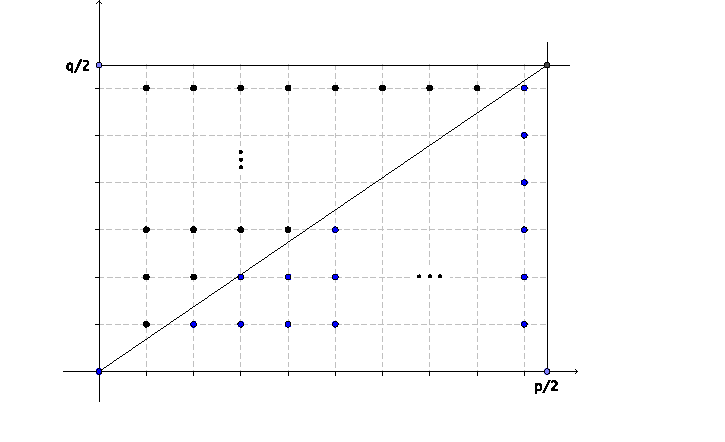
\includegraphics[scale=1]{./iliustracijos/skteorija/gardele.pdf} 
\end{center}
\end{proof}

Kvadratinio apverčiamumo teorema galioja tik nelyginiams pirminiams.
Dvejetą reikia nagrinėti atskirai:

\begin{thm} Liekana $2$ yra kvadratinė moduliu $p$ tada ir tik tada, kai
  $p\equiv \pm1 \m{8},$ t.y. $\lez{2}{p} = (-1)^\frac{p^2 -1}{8}$.
\end{thm}

\begin{proof}[Įrodymas]
  Pasinaudosime kvadratinio apverčiamumo teoremos įrodymo metu gauta lygybe
  (dar vadinama Gauss lema) atveju $a=2$:
  $$\lez{2}{p} \equiv (-1)^{\mu_2} \m{p}.$$
  Pasirodo, šiuo atveju galima suskaičiuoti tikslią $\mu_2$ reikšmę,
  priklausomai nuo pirminio $p$ dalybos iš $8$ liekanos. Nagrinėkime $4$
  atvejus:

  \begin{itemize}
    \item[$p = 8k + 1$ -- ] Šiuo atveju bus iš viso $4k$ liekanų, padauginus
      jas iš dviejų, $2k$ bus nedidesnės nei $4k$ ir $2k$ bus didesnės.
      Vadinasi, $\mu$ bus lygus $2k$ ir $\lez{2}{p} = 1$.
    \item[$p = 8k + 3$ -- ] Šiuo atveju bus iš viso $4k + 1$ liekana,
      padauginus jas iš dviejų, $2k$ bus nedidesnės nei $4k+1$ ir $2k+1$ bus
      didesnės. Vadinasi $\mu$ bus lygus $2k+1$ ir $\lez{2}{p} = -1$.
    \item[$p = 8k + 5$ -- ] Šiuo atveju bus iš viso $4k + 2$ liekanos,
      padauginus jas iš dviejų, $2k+1$ bus ne didesnės nei $4k+2$, ir $2k+1$
      bus didesnės. Vadinasi, $\mu$ bus lygus $2k+1$ ir $\lez{2}{p} = -1$.
    \item[$p = 8k + 7$ -- ] Šiuo atveju bus iš viso $4k + 3$ liekanos,
      padauginus jas iš dviejų, $2k+1$ bus ne didesnės nei $4k+3$ ir $2k+2$
      bus didesnės. Vadinasi, $\mu$ bus lygus $2k+2$ ir $\lez{2}{p} = 1$.  
  \end{itemize}
\end{proof}

Kvadratinio apverčiamumo teorema taip vadinasi ne be reikalo. Jos dėka
užuot skaičiavus $\lez{p}{q}$, galima skaičiuoti $\lez{q}{p}$. Geriau
įsižiūrėjus į teoremos formuluotę pasidaro aišku, kad šių dviejų Ležandro
simbolių reikšmės sutaps, jei bent vienas iš $p$, $q$ duos dalybos liekaną
$1$ moduliu $4$, ir bus skirtingos, jei abiejų pirminių dalybos liekanos
moduliu $4$ bus lygios $3$. Pažiūrėkime, kaip tai atrodo praktiškai.

\subsubsection{Pavyzdžiai}

\begin{pavnr}
  Raskite, ar $23$ yra kvadratinė liekana moduliu $37$.
\end{pavnr}

\begin{sprendimas}
  Abu duoti skaičiai yra nelyginiai pirminiai, todėl galime taikyti
  kvadratinio apverčiamumo teoremą. Kadangi $37 \equiv 1 \m{4}$, tai
  gausime
  $$\lez{23}{37}\lez{37}{23} = 1\implies \lez{23}{37} = \lez{37}{23}.$$
  Pagrindinė nauda, kurią gauname iš apvertimo, yra ta, kad dabar skaitiklis
  yra didesnis už vardiklį, tad galime jį redukuoti moduliu. Kadangi $37
  \equiv 14 \m{23}$, tai gausime $$\lez{37}{23} = \lez{14}{23}.$$ 
  Redukavę, pritaikome lygybę $\lez{ab}{p} = \lez{a}{p}
  \lez{b}{p}$: $$\lez{14}{23} = \lez{2}{23} \lez{7}{23}.$$
  Pirmąjį iš dauginamųjų galime iš karto suskaičiuoti. Kadangi $23 \equiv
  -1 \m{8}$, tai $\lez{2}{23}=1$. Antrąjį vėl apversime (šį kartą gausime,
  kad apverstasis yra priešingo ženklo, nes $7 \equiv 23 \equiv 3 \m{4}$):
  $$\lez{7}{23} = -\lez{23}{7} = -\lez{2}{7}.$$ 
  Kadangi $7 \equiv -1\m{8}$, tai gauname, kad $\lez{2}{7}=1$, vadinasi,
  viską sujungę gausime $\lez{23}{37}=-1$, t.y. $23$ nėra kvadratinė
  liekana moduliu $37$.
\end{sprendimas}

\begin{pavnr}
  Raskite, ar $41$ yra kvadratinė liekana moduliu $61$.
\end{pavnr}

\begin{sprendimas}
  Darysime tą patį, ką ir praeitame pavyzdyje:
  $$\lez{41}{61}=\lez{61}{41}=\lez{20}{41}=\lez{2}{41}^2\lez{5}{41}=\lez{41}{5}=\lez{1}{5}
  = 1.$$
\end{sprendimas}

\begin{pavnr}
  Raskite, moduliu kurių pirminių, $3$ yra kvadratinė liekana.
\end{pavnr}

\begin{sprendimas}
  Ieškosime, kada $\lez{3}{p}$ yra lygus vienetui. Taikysime kvadratinio
  apverčiamumo teoremą. Kadangi $3 \equiv 3 \m{4}$, tai
  $$\lez{3}{p} = (-1)^\frac{p-1}{4}\lez{p}{3}.$$
  Sandauga bus lygi $1$, kai abu daugikliai lygus $1$ arba $-1$. Kadangi
  $\lez{p}{3}$ lygus $1$, kai $p\equiv 1\m{3}$ ir $-1$, kai $p\equiv
  2\m{3}$, tai gausime, kad mums tinka pirminiai skaičiai, tenkinantys
  sistemas:
  $$\begin{cases}
    p \equiv 1 \m{4}\\
    p \equiv 1 \m{3}
  \end{cases}
  \text{ ir } \phantom{ir}
  \begin{cases}
    p\equiv -1 \m{4}\\
    p\equiv -1 \m{3}
  \end{cases}$$
  Tokiais bus pirminiai $p\equiv \pm 1 \m{12}$.
\end{sprendimas}

\begin{pavnr}
  Kokie pirminiai skaičiai gali būti daugianario $x^2 + 5$ dalikliais?
  (Skaičių vadiname daugianario $q(x)$ dalikliu, jei su kuria nors $x$
  reikšme $q(x)$ iš jo dalijasi.)
\end{pavnr}

\begin{sprendimas}
  Jei $p$ yra daugianario $x^2 + 5$, tai su kažkokia $x$ reikšme bus
  tesinga lygybė $$x^2 + 5 \equiv 0 \m{p} \iff x^2 \equiv -5 \m{p},$$ t.y.
  $-5$ turės būti kvadratinė liekana moduliu $p$. Tarę, kad $p\neq 5$,
  skaičiuojame:
  $$\lez{-5}{p}=\lez{-1}{p}\lez{5}{p}=(-1)^\frac{p-1}{2}\lez{p}{5}.$$
  Sandauga bus lygi $1$, jei $p\equiv 1\m{4}$ ir $p\equiv \pm1 \m{5}$, arba
  jei $p\equiv -1 \m{4}$ ir $p \equiv \pm2 \m{5}.$ Išsprendę lyginių
  sistemas, randame, kad tiks $p\equiv 1 \m{20}$, $p\equiv 3 \m{20}$,
  $p\equiv 7 \m{20}$, $p\equiv 9 \m{20}$ bei atskiras atvejis $p=5$.
\end{sprendimas}

\subsubsection{Uždaviniai}

\begin{enumerate} 
  \item Raskite $\lez{79}{101}$.  
    %Skaičiuokime:$$\lez{79}{101} =\lez{101}{79} =\lez{22}{79}
    %=\lez{2}{79}\lez{11}{79} =-\lez{79}{11} =-\lez{2}{11} = 1.$$
  \item Įrodykite, kad jei pirminis $p > 3$ dalo skaičių $a^2 + 12$, tai tuomet
    $p \equiv 2 \m{3}$.  
    %Jei $p|a^2 + 12$, tai $a^2 \equiv -12 \m{p}.$ Ieškome moduliu kurių
    %pirminių $p$, liekana $-12$ bus kvadratinė:
    %$$\lez{-12}{p} = \lez{-1}{p}\lez{2}{p}^2\lez{3}{p} =
    %(-1)^\frac{p-1}2(-1)^\frac{p-1}{2}\lez{p}{3} = \lez{p}{3}.$$
  \item Įrodykite, kad iš visų nelygių nuliui liekanų moduliu pirminio $p$, pusė
    yra kvadratinės ir pusė nekvadratinės. 
    %Kvadratinėmis bus lyginiai generatoriaus laipsniai, o nekvadratinėmis -
    %nelyginiai, tad tikrai pusė bus tokių ir pusė kitokių.
  \item Nustatykite, moduliu kurių pirminių, $6$ yra kvadratinė liekana. 
    %Palikę nuošalyje atvejus $p=2$ ir $p=3$ ieškome kitų:
    %$$\lez{6}{p} = \lez{2}{p}\lez{3}{p} =
    %(-1)^\frac{p^2-1}{8}(-1)^\frac{p-1}{2}\lez{p}{3}.$$
    %Sandauga bus lygi $1$ kai $p\equiv 1, 3 \m{8}$ ir $p\equiv 1\m{3}$,
    %arba kai $p\equiv 5, 7 \m{8}$ ir $p\equiv 2\m{3}$. Sujungę gauname,
    %kad tiks $p \equiv \pm 1 \m{24}$ ir $p \equiv \pm 5\m{24}$.
  \item \text{[LitMo 1987]}Skaičius $N$ lygus pirmųjų $n\geq 2$ pirminių
    skaičių sandaugai. Įrodykite, kad nei vienas iš skaičių $N-1$ ir
    $N+1$ nėra natūraliojo skaičiaus kvadratas.
    %Skaičius $N$ dalinsis iš $2$ ir $3$ bet nesidalins iš $4$, todėl
    %$N - 1 \equiv 2 \m{3}$ ir $N+1 \equiv 3 \m{4}$. Tačiau nei $2$ moduliu
    %$3$, nei $3$ moduliu $4$ nėra kvadratinės liekanos.
  \item Įrodykite, kad, kaip ir įprastai, kvadratinė lygtis
    $ax^2+bx+c\m{p}, a\not \equiv 0, p\neq 2$ turės sprendinių tada ir tik tada, kai
    diskriminantas $b^2-4ac$ bus kvadratinė liekana (įskaitant nulį) moduliu $p$.
    %Pakanka perrašyti lygtį kaip $(x+\frac{b}{2a})^2 \equiv
    %\frac{b^2-4ac}{4a^2}\m{p}$.
  \item \text{[Brazil 2003]} Raskite mažiausią pirminį, kuris dalo
    daugianarį $n^2 + 5n +23$.
    %Daugianario reikšmės visuomet nelyginės, tad pakaks nagrinėti moduliu
    %kurio nelyginio pirminio diskriminantas $-67$ yra kvadratinė liekana.
    %Pirmasis toks pirminis bus $17$, ir jis tikrai daugianarį dalins,
    %pavyzdžiui, kai įstatysime reikšmę $n=-2$.
  \item Įrodykite, kad jei pirminis $p\equiv 3 \m{4}$, tai iš $p|a^2 + b^2$
    seka $p^2|a^2 + b^2$.
    %Įrodysime, kad jei $p|a^2 + b^2$, tai $p|a$ ir $p|b$. Tarkime
    %priešingai, tegu, pavyzdžiui, $p\nmid b$. Tuomet iš $a^2 + b^2 \equiv 0\m{p}$
    %gausime $(ab^{-1})^2\equiv -1 \m{p}$ -- prieštara, nes $-1$ nėra
    %kvadratinė liekana moduliu pirminių duodančių liekaną $3$ moduliu
    %$4$.
  \item Tegu pirminis $p = 4n+1$. Įrodykite, kad visi $n$ dalikliai yra
    kvadratinės liekanos moduliu $p$.
    %Imkime bet kurį pirminį $n$ daliklį $q$. Jei $q$ nelyginis, tai pagal
    %kvadratinio apverčiamumo teoremą $\lez{q}{p} = (-1)^{2n\cdot
    %\frac{q-1}{2}} \lez{p}{q}= 1\cdot \lez{1}{q} = 1.$ Jei $q$ lyginis,
    %t.y. $2$, tai tuomet $p \equiv 1 \m{8}$ ir $\lez{2}{p} = 1$.Kadangi
    %bet koks $n$ daliklis bus sandauga pirminių daliklių, t.y. kvadratinių
    %liekanų, tai ir jis pats bus kvadratinė liekana.
  \item Įrodykite, kad kvadratinių liekanų sandauga lygsta $1$ moduliu $p$, kai
    $p\equiv 3\m{4}$, ir $-1$, kai $p\equiv 1\m{4}$.
    %Nagrinėkime du atvejus. Kai $p = 4k + 3$, gausime iš viso $2k + 1$
    %dauginamąjį. Kadangi $-1$ nėra kvadratinė liekana moduliu $p$, tai
    %tarp dauginamųjų bus tik viena liekana, kuri yra pati sau atvirkštinė
    %(liekana $1$).  Visos likusios bus atvirkštinės poromis (kvadrato
    %atvirkštinė yra kvadratas), tad sudauginę iš ties gausime $1$.
    %
    %Kai $p=4k+1$, gausime iš viso $2k$ dauginamųjų. Kadangi $-1$ šiuo
    %atveju jau yra kvadratinė liekana, tai bus dvi liekanos, kurios yra
    %sau atvirkštinės ($1$ ir $-1$). Likusios vėl bus atvirkštinės poromis,
    %tad visų sandauga bus lygi $-1$.
  \item Įrodykite, kad $1^2 3^2 5^2\cdots (p-2)^2 \equiv
    (-1)^{(p+1)/2}\m{p}.$
    %Pastebėkime, kad duota sandauga yra visų kvadratinių liekanų moduliu
    %$p$ sandauga. Iš ties -- iš viso yra $(p-1)/2$ liekanų, visos jos
    %kvadratinės, ir jokios dvi nesutampa, nes jei $a^2 \equiv b^2 \m{p}$,
    %tai arba $a\equiv b\m{p}$ arba $a\equiv -b\m{p}$. Pastaroji lygybė
    %negali būti teisinga, nes ir $a$ ir $b$ nelyginiai skaičiai tarp $1$
    %ir $p-2$. Lieka pasinaudoti praeitu uždaviniu.
  \item Pasinaudoję lygybe $x^4 + 4 = ((x+1)^2+1)((x-1)^2+1)$ parodykite,
    kad $-4$ bus \textit{bikvadratinė} liekana mod $p$ tada ir tik tada,
    kai $p \equiv 1$ mod $4$. ($a$ yra bikvadratinė liekana, jei egzistuoja
    sprendinys $x^4 \equiv a$ mod $p$) 
    %Liekana $-4$ bus bikvadratinė moduliu $p$, kai lygtis $x^4 + 4 \equiv
    %0 \m{p}$ turės sprendinį. Pasinaudoję duota lygybe gauname, kad taip
    %bus tada ir tik tada, kai sprendinį turės viena iš lygčių $(x\pm1)^2 +
    %1=0$, kas yra ekvivalentu $-1$ buvimui kvadratine liekana moduliu $p$. 
  \item Įrodykite, kad pirminiai daugianario $x^4 - x^2 + 1$ dalikliai
    lygsta $1$ mod $12$. 
    %Jei pirminis $p$ dalo duotą reiškinį, tai tuomet $x^4 - x^2 + 1
    %\equiv 0 \m{p}$. Perrašykime šią lygybę dviem būdais: $(x^2-1)^2\equiv
    %-x^2\m{p}$ ir $(x^2+1)^2 \equiv -3x^2\m{p}$. Iš pirmosios gausime, kad
    %$-1$ yra kvadratinė liekana moduliu $p$, t.y. $p \equiv 1\m{4}$, o iš
    %antrosios, kad $3$ yra kvadratinė liekana moduliu $p$, t.y. $p \equiv
    %1\m{3}$.
  \item Įrodykite, kad visi pirminiai yra daugianario $x^6 - 11x^4 + 36x^2
    - 36$ dalikliai.
    %Išskaidę daugianarį dauginamaisiais gauname $(x^2 - 2)(x^2-3)(x^2-6).$
    %Pirminis $p$ nedalins jo, kai ir $2$, ir $3$, ir $6$ bus nekvadratinės
    %liekanos. Tačiau to būti negali, nes dviejų nekvadratinių liekanų
    %sandauga yra kvadratinė liekana.
  \item Tegu pirminis $p\equiv 3$ mod $4$, ir $q=2p+1$ taip pat pirminis.
    Įrodykite, kad $q|2^p -1$.
    %Kadangi $q$ pirminis, tai $q|2^{q-1}-1$, t.y. $2^{2p}\equiv 1\m{q}$.
    %Vadinasi, $2^p$ bus lygus arba $1$ arba $-1$ moduliu $q$. Parodysime,
    %kad atrasis variantas negalimas. Kandagi $p\equiv 3\m{4}$, tai
    %$q\equiv 7\m{8}$, bet tuomet $2$ yra kvadratinė liekana moduliu
    %$q$, o $-1$ nėra, kas prieštarautų $2^p\equiv -1 \m{q}$. 
  \item Žinoma, kad jei pirminis $p \equiv 1$ mod $4$, tai jis užrašomas kaip
    dviejų kvadratų suma $p = a^2 + b^2$. Tegu $a$ -- nelyginis dėmuo.
    Įrodykite: \\
      a) $\lez{a}{p} = 1$;\\
      b) $\lez{a+b}{p} = (-1)^\frac{(a+b)^2 - 1}{8}$;\\
      c) $(a+b)^2 \equiv 2ab\m{p}$;\\
      d) $(a+b)^\frac{p-1}{2} \equiv (2ab)^\frac{p-1}{4}\m{p}$.\\
    Tegu $f$ toks, kad $b\equiv af \m{p}$. Įrodykite, kad $f^2 \equiv -1$
    mod $p$ ir kad $2^\frac{p-1}{4} \equiv f^{ab/2} \m{p}$. 

    Įrodykite, kad $2$ yra bikvadratinė liekana moduliu $p$ tada ir tik tada,
    kai $p$ užrašomas kaip $A^2 + 64B^2$.
    %a) Tegu $q$ pirminis $a$ daliklis (pagal sąlygą
    %nelyginis). Kadangi $p \equiv b^2 \m{q}$ ir $p\equiv 1 \m{4}$, tai
    %$\lez{q}{p}=\lez{p}{q}=\lez{b^2}{q}=1.$ Kadangi visi pirminiai $a$
    %dalikliai yra kvadratinės liekanos, tai ir $a$ bus kvadratinė
    %liekana.\\
    %b) Tegu $q$ pirminis $a+b$ daliklis. Užsirašę lygybę
    %$p=a^2+b^2 = (a+b)(a-b) +2b^2$ matome, kad $p\equiv 2b^2\m{q}$, arba
    %$\lez{q}{p}=\lez{p}{q}=\lez{2}{q}$. Jei $a+b$ turi lyginį skaičių
    %pirminių daliklių (skaičiuojant kartotinumus), kurie lygsta $\pm 3$
    %moduliu $8$, tai tuomet $\lez{a+b}{p}=1$ ir $a+b \equiv \pm 1
    %\m{8}$, o jei nelyginį, tai tuomet $\lez{a+b}{p}=-1$ ir $a+b\equiv \pm
    %3\m{8}$.\\
    %c) Duota lygybė seka iš $(a+b)^2 -2ab = p$.\\
    %d) Pakanka prieš tai gautą lygybę pakelti laipsniu $(p-1)/4$.
    %
    %Užrašę lygybę $a^2 \equiv -b^2 \equiv a^2f^2 \m{p}$ ir suprastinę
    %gausime $f^2\equiv -1 \m{p}.$ Sujungę šį pastebėjimą su antra ir
    %ketvirta lygybėmis gausime 
    %\begin{align*}
    %f^\frac{(a+b)^2 - 1}{4}\equiv (-1)^\frac{(a+b)^2 - 1}{8}\equiv
    %(a+b)^\frac{p-1}{2} \equiv (2ab)^\frac{p-1}{4} & \equiv
    %(2a^2f)^\frac{p-1}{4} \\ &\equiv 2^\frac{p-1}{4} f^\frac{p-1}{4}
    %\m{p}, 
    %\end{align*}
    %ką suprastinę gausime $2^\frac{p-1}{4} \equiv f^{ab/2}
    %\m{p}$. Galiausiai lieka pastebėti, kad $f^{ab/2} \equiv 1 \m{p}$ tik
    %tada, kai $b$ dalijasi iš $8$, kas ir reiškia, kad $p$ užrašomas kaip
    %$A^2 + 64B^2.$
  \item \text{[JBMO 2007]} Įrodykite, kad jei $p$ yra pirminis, tai $A = 7p
    + 3^p - 4$ nėra pilnas kvadratas.
    %Kai $p=2$ tai $A$ nėra kvadratas, tad tarkime, kad $p\geq 3$ . Pagal
    %Ferma teoremą $7p + 3^p - 4\equiv -1 \m{p}.$ Jei $A$ kvadratas, tai
    %$-1$ kvadratinė liekna moduliu $p$, todėl $p=4k+1$. Tačiau tuomet
    %$A \equiv 7+(-1)-4 \equiv 2 \m{4},$ ko būti negali, nes 2 nėra
    %kvadratinė liekana moduliu 4. 
  \item \text{[Kazakhstan 2004]} Raskite visus pirminius $p$, su kuriais
    lygtis $x^2+y^2=2003+pz$ turi sveikųjų sprendinių.
    %Parodysime, kad lygtis visuomet turi sprendinių. Tarkime priešingai,
    %tegu su kažkokiu $p$ lygtis sprendinių neturi, t.y. su visomis $x$ ir
    %$y$ reikšmėmis $x^2 + y^2 \not \equiv 2003 \m{p}$, arba $x^2 \not
    %\equiv 2003-y^2 \m{p}$. Kadangi moduliu $p$ lygiai $\frac{p+1}{2}$
    %pusiau liekanų yra kvadratinės (su nuliu), tai ir kairė ir dešinė
    %lygties pusės įgys po $\frac{p+1}{2}$ skirtingų reikšmių. Kadangi
    %$\frac{p+1}{2} + \frac{p+1}{2} > p$, tai bent dvi jos sutaps -
    %prieštara.
  \item \text{[Vietnam 2004]} Tegu $S(n)$ skaičiaus $n$ skaitmenų suma.
    Raskite mažiausią galimą $S(m)$ reikšmę, jei $m$ dalijasi iš $2003$.
    %Skaičiaus $m$ skaitmenų suma negali būti lygi $1$, parodysime, kad
    %negali būti lygi ir dviem. Tarkime priešingai, tuomet egzistuos tokios
    %$a$ ir $b$ reikšmės, su kuriomis $10^a + 10^b$ dalinsis iš $2003$, t.y.
    %$10^a \equiv -10^b \m{2003}.$ Kadangi $10$ yra kvadratinė liekana
    %moduliu $2003$ ($\lez{10}{2003} = \lez{2}{2003}\lez{5}{2003} =
    %-\lez{3}{5} = 1$), tai gauname, kad ir $-1$ yra kvadratinė liekana
    %moduliu $2003$; prieštara. 
    %
    %Parodyti, kad $S(m)=3$, nėra labai paprasta, nes tenka
    %dauginti gana nemažus skaičius, norint įsitikinti, kad $10$ laipsniai
    %įgyja pakankamai daug skirtingų liekanų. Konkrečiau, norint parodyti,
    %kad $10$ eilė moduliu $2003$ yra $1001$ reikia parodyti, kad
    %$10^{77}, 10^{91}$ ir $10^{143}$ nelygsta vienetui. Greičiausia yra
    %rasti laipsnius $10^7, 10^{14}, 10^{28}, 10^{56}, 10^{112}$, tuomet
    %gausime, kad $10^{77} \equiv 10^710^{14}10^{56}$, $10^{91} \equiv
    %10^{77}10^{14}$, $10^{143} = 10^{112}10^{28}10^3$. 
    %Parodžius tai, lieka pastebėti, kad tuomet $10$ laipsniais galėsime
    %užrašyti visas kvadratines liekanas, tarp jų ir $1600, 400$ ir
    %$3$.
 \end{enumerate}

\newpage
%Copyrighted by Paulius Šarka, 2010. Some rights reserved.

\section{Diofantinės lygtys}

Lygtys yra vadinamos diofantinėmis, kai yra ieškoma jų sveikųjų
sprendinių. Šiame skyrelyje apžvelgsime keletą metodų padedančiu jas
spręsti. Atkreipsime dėmesį, kad, skirtingai nuo įprastų lygčių,
'spręsti' dažniausiai yra bandyti įrodyti, kad lygtis sprendinių neturi,
arba jei ir turi, tai labai specifinius.  

\subsection{Dvi lygties pusės}

Pradėsime nuo trijų pagrindinių principų, besiremiančių labai bendru
pastebėjimu:

\smallskip
\begin{center}\emph{Lygybės abi pusės yra vienodo dydžio, vienodai skaidomos
dauginamaisiais ir duoda vienodas liekanas dalijamos iš natūraliųjų
skaičių.}\end{center}
\smallskip

\subsubsection{Dydis}

Pradėkime nuo pavyzdžių. Išspręsime tris paprastas lygtis.
\begin{pav} 
  Raskite lygties $x^2 = x + 2$ sveikuosius sprendinius.
\end{pav}

\begin{sprendimas}
  Ši lygtis yra kvadratinė, ir ją galima išspręsti įprastai, tačiau minutėlei tą
  pamirškime ir pabandykime pasinaudoti tuo, kad kairioji pusė beveik visada yra didesnė
  už dešiniąją. Įvertinkime - kai $x\geq 3$, tai $x^2 \geq 3x \geq x + 6 >
  x+2$, o kai $x\leq -2$, tai $x^2 > 0 \geq x+2$, tad vienintėliai sveikieji
  skaičiai, kurių negalėjome atmesti samprotaudami apie skirtingus lygties
  pusių dydžius, yra $-1, 0, 1$ ir $2$. Lieka tik patikrinti, kurie iš jų
  tinka, ir rasti, kad lygties sprendiniai yra $-1$ ir $2$. 
\end{sprendimas}

\begin{pav}
  Raskite lygties $x^2 + y^2 = 100$ sveikuosius sprendinius.
\end{pav}

\begin{sprendimas}
  Sveikųjų skaičių kvadratai yra visuomet neneigiami ir auga palyginti
  sparčiai. Šios lygties atveju, kaip tik tuo ir pasinaudosime - jei $x$ arba
  $y$ yra moduliu didesni už $10$, tai kairioji pusė tampa didesnė už
  $100$. Atkreipę dėmesį į tai, kad jei $(x,y)$ yra sprendinys tai ir
  $(\pm x,\pm y)$ yra sprendinys gauname, kad užtenka patikrinti $x$ 
  reikšmes nuo $0$ iki $10$. Tai padaryti nesunku - randame, kad sprendiniai
  bus $(0,10)$, $(6,8)$, $(8,6)$, $(10,0)$ su visomis skirtingomis ženklų
  kombinacijomis. 
\end{sprendimas}

\begin{pav}
  Raskite lygties $xy = x+y$ sveikuosius sprendinius.
\end{pav}

\begin{sprendimas}
  Dviejų sveikųjų skaičių sandauga beveik visada yra didesnė už sumą.
  Pasinaudosime tuo, tačiau pirmiausia atmeskime neigiamus atvejus. Aišku,
  kad abu ir $x$, ir $y$, negali būti neigiami, nes tuomet sandauga bus
  teigiama, o suma neigiama. Negali būti ir vienas neigiamas, vienas
  teigiamas, pvz. $x>0$, $y<0$, nes tuomet $xy \leq y < y + x$. Tad ieškokime
  sprendinių, kuriuose $x\geq 0$ ir $y\geq 0$ ir taip pat neprarasdami
  bendrumo tarkime, kad $y$ yra nemažesnis nei $x$. Parodysime, kad
  $x$ negali būti didesnis už $2$. Iš ties, jei $x\geq 3$, tai $xy \geq 3y >
  y + x$. Vadinasi $x$ gali įgyti tik reikšmes $0$, $1$ ir $2$. Patikrinę
  randame sprendinius $(0,0)$ ir $(2,2)$.
\end{sprendimas}

Bandant įvertinti reiškinių dydžius, natūraliai praverčia algebrinės
nelygybės ir supratimas apie funkcijų didėjimą, argumentui artėjant į
begalybę (pavyzdžiui, didesnio laipsnio daugianaris nuo kažkurios reikšmės
visuomet įgis didesnes reikšmes už mažesnio laipsnio daugianarį). Puiki ir
paprasta šių idėjų iliustracija - 1988 metų Lietuvos matematikos olimpiados
uždavinys:
\begin{pav} \text{\emph{[LitMo 1988]}} Išspręskite natūraliaisiais skaičiais lygtį
  $3x^2 + 2y^2 = 4xy + 2x.$
\end{pav}
\begin{sprendimas}
  Parodysime, kad kairioji pusė beveik visada yra didesnė už dešiniąją. Iš
  ties - pagal aritmetinio-geometrinio vidurkio nelygybę $2x^2 +
  2y^2 \geq 4xy$, ir $x^2 > 2x$, kai $x>2$. Vadinasi, lieka patikrinti tik
  dvi reikšmes - $x=1$ ir $x=2$. Tinka tik antroji, randame sprendinį
  $(2,2)$.
\end{sprendimas}

Dažniausiai, kaip ir turi būti olimpiadiniuose uždaviniuose, lygybės pusių
dydžių skirtumo idėja būna užmaskuota ir reikia akylumo norint ją įžiūrėti.
Pavyzdžiui:

\begin{pav} \text{\emph{[LitKo 2009]}} Raskite lygties
  $(a^2 - 9b^2)^2 - 33b = 16$ sveikuosius neneigiamus sprendinius.
\end{pav}

\begin{sprendimas}
Šis uždavinys organizatoriams greičiausiai pasirodė kiek sunkokas, todėl
olimpiadoje buvo suformuluotas kaip dviejų dalių, pirmoji iš kurių prašė
įrodyti, kad visi sprendiniai tenkina nelygybę $|a-3b|\geq 1$. Įrodyti tai
labai paprasta, tačiau įžiūrėti užuominą gerokai sunkiau. Paprasčiausia tai
padaryti turbūt būtų išskaidant pirmąjį dėmenį dauginamaisiais: $(a^2 -
9b^2)^2 = (a-3b)^2(a+3b)^2$, tuomet
$$(a-3b)^2(a+3b)^2 \geq (a+3b)^2\geq 9b^2.$$
Vadinasi, kairioji lygties pusė yra ne mažesnė nei $9b^2 - 33b=(9b-33)b$, bet
šio reiškinio reikšmė yra didesnė už $16$ su visomis $b$ reikšmėmis
viršijančiomis $4$, vadinasi lieka patikrinti vos keletą reikšmių.

Tačiau atidėkime šį sprendimą į šalį ir dar kartą pažvelkime į lygtį,
bandydami kiek kitaip įvertinti kairiosios pusės dydį. Priežastis, dėl
kurios $(a^2-9b^2)^2$ yra beveik visada daug didesnis už $33b$ yra
ta, kad skirtumas tarp kvadratų yra pakankamai didelis. Išties, jei
$a^2$ nėra lygus $9b^2$, tai arčiausiai (tuomet skirtumas mažiausias) jis
gali būti tik tuomet, kai yra artimiausiai esantis kvadratas. O
artimiausias kvadratas yra $(3b-1)^2$, bet net tuomet skirtumas visvien yra
$6b-1$, o $(6b-1)^2 - 33b$ yra didesnis už $16$ su visomis $b$ reikšmėmis
didesnėmis už $1$! Lieka vos du atvejai, iš kurių gauname po sprendinį:
$(4,0)$ ir $(4,1)$.
\end{sprendimas}

Viena (labai svarbi!) iš samprotavimo apie dydį variacijų -„įterpimo tarp
kvadratų' triukas. Norint parodyti, kad sveikasis skaičius nėra kvadratas,
užtenka parodyti, kad jis yra tarp dviejų gretimų kvadratų ir nė vienam iš
jų nelygus. Ši strategija tinka, žinoma, ir aukštesniems laipsniams.

\begin{pav} Raskite lygties $y^2 = x^2 + x + 1$ sveikuosius sprendinius.
\end{pav}

\begin{sprendimas}
Kairioji lygties pusė yra kvadratas, o dešinioji beveik visada nėra, nes
$x^2 < x^2 + x + 1 < (x+1)^2$ (arba $(x+1)^2 < x^2 + x + 1 < x^2$, jei $x$
neigiamas).  Vienintelės $x$ reikšmės, su kuriomis šios nelygybės nėra
teisingos yra $x=-1$ ir $x=0$, gauname sprendinius $(-1, \pm 1)$ ir $(0,
\pm 1)$.
\end{sprendimas}

\subsubsection{Liekanos}

Nagrinėjant lygtį moduliu pasirinkto skaičiaus, apribojimą, kad abi lygybės
pusės turi duoti vienodą liekaną moduliu to skaičiaus, dažnai galima
perkelti į apribojimą ieškomiems sprendiniams. Kartais tas apribojimas būna
pakankamas, kad galėtume visiškai išspręsti lygtį, bet dažniau jis tampa
pagalbine informacija, kuri tampa naudinga sujungus ją su kitomis idėjomis.
Pradėkime nuo paprasčiausių atvejų, kai nagrinėjant lygtį moduliu tinkamai
parinkto skaičiaus ji išsisprendžiama iki galo.

\begin{pav} Raskite lygties $x^2 = 3y - 1$ sveikuosius sprendinius.
\end{pav}

\begin{sprendimas}
Nagrinėkime šią lygtį moduliu $3$. Norint, kad $(x,y)$ būtų sprendinys,
abiejų lygybės pusių dalybos liekana iš $3$ turi būti vienoda. Dešinės
pusės dalybos liekana bus $-1$, o kairės, priklausomai nuo $x$, arba
$0$, arba $1$. Gavome, kad su jokiais $(x,y)$ jos nesutaps, todėl lygtis
sprendinių neturi.
\end{sprendimas}

\begin{pav} Raskite lygties $x^2 = 2^n - 1$ sveikuosius sprendinius. 
\end{pav}

\begin{sprendimas}
  Nagrinėkime lygtį moduliu $4$. Dešinė pusė, kad $n>1$, lygsta $-1$ moduliu
  $4$, o kairė $0$ arba $1$. Kadangi liekanos nesutampa, tai lieka tik
  atvejai $n\leq 1$, kuriuos patikrinę ($n$ negali būti neigiamas, nes
  tuomet $2^n$ nebūtų sveikasis) randame sprendinius $n=1, x=\pm 1$ ir
  $n=0, x=0$. 
\end{sprendimas}

\begin{pav} Raskite lygties $2 + x^2 + x^3 = 6^n$ sveikuosius sprendinius
\end{pav}

\begin{sprendimas}
  Nagrinėkime lygtį moduliu $3$ arba moduliu $5$, arba moduliu $7$. Visais
  trimis atvejais lengva įsitikinti, kad abi pusės duoda skirtingas
  liekanas.
\end{sprendimas}

Kaip jau užsiminėme, lygties nagrinėjimas moduliu (arba sprendimas moduliu)
dažniausiai yra tik dalis sprendimo. Pavyzdžiui:

\begin{pav}
  \text{\emph{[Lietuvos TST 2009]}} Raskite lygties $x^3 + x^2 =
  16 + 2^y$ natūraliuosius sprendinius.
\end{pav}

\begin{sprendimas}
  Nagrinėkime lygtį moduliu $7$. Kairioji pusė gali įgyti liekanas $0, 1,
  2, 3, 5$, o dešinioji $3, 4$ ir $6$. Vienintėlė bendra liekana yra $3$, ir
  ji įgyjama kai $y$ dalijasi iš $3$. Panaudokime gautą informaciją -
  pažymėkime $y=3a$ ir perrašykime lygtį kaip $$(2^{a})^3 = x^3 + x^2 -
  16.$$ Lieka pastebėti, kad galime pritaikyti įterpimo tarp kubų įdėją: su
  visais $x>4$ turime $$x^3 < x^3 + x^2 -16 < (x+1)^3,$$ vadinasi, lieka
  patikrinti tik keturias $x$ reikšmes. Randame vienintelį sprendinį
  $(4,6)$.
\end{sprendimas}

\begin{pav}
  \text{\emph{[MEMO 2009, Aivaras Novikas]}} Raskite lygties $2^x + 2009 =
  3^y5^z$ neneigiamus sveikuosius sprendinius.
\end{pav} 
 
\begin{sprendimas}
  Pirmiausia įsitikinkime, kad $x$ negali būti mažesnis už $3$. Išties -
  įstačius reikšmes $0, 1, 2$ kairiojoje pusėje gauname $2010, 2011,
  2013$ ir nė vienas iš šių skaičių neišsiskaido tik į trejeto ir penketo
  laipsnius. Tad tarkime, kad $x\geq 3$. Įrodysime, kad visi trys
  $x, y, z$ turi būti lyginiai.
  \begin{itemize}
    \item[$x$ -] Jei $y>0$, tai nagrinėkime lygtį moduliu $3$ gausime
      $(-1)^x - 1 \equiv 0$, vadinasi $x$ lyginis. Jei $y=0$, tai
      $z>0$, tuomet nagrinėkime lygtį moduliu $5$. Gausime $2^x - 1 \equiv
      0$, vadinasi $x$ dalijasi iš $4$, t.y. yra lyginis.
    \item[$y$ -] nagrinėkime lygtį moduliu $4$. Kadangi $x>2$, tai gausime
      $1 \equiv (-1)^y$, vadinasi $y$ lyginis.
    \item[$z$ -] nagrinėkime lygtį moduliu $8$. Kadangi $x>2$ ir $y$ lyginis,
      tai gausime $1 \equiv 5^z$, vadinasi $z$ lyginis.
  \end{itemize}
  Pažymėję $x=2a$, $y=2b$, $z=2c$ galime lygtį pertvarkyti į $$2009 =
  (3^b5^c - 2^a)(3^b5^c + 2^a).$$ Kadangi $2009$ išsiskaido kaip $7^2\cdot
  41$, tai į dviejų dauginamųjų sandaugą galime jį išskaidyti tik trim
  būdais: $1\cdot 2009$, $7\cdot 287$ ir $41\cdot 49$. Vienintelis
  išskaidymas, kurio dauginamieji skiriasi per dvejeto laipsnį yra
  $41\cdot 49$, iš kur randame vienintėlį sprendinį $(4,4,2)$. 
\end{sprendimas}

Lygties sprendimą moduliu visuomet verta prisiminti sprendžiant diofantines
lygtis ir ypač tas, kuriose iš pirmo žvilgsnio nesimato jokių silpnų vietų.
Neretai verta spręsti lygtį moduliu nedidelių skaičių (pvz. $2, 3, 4, 5, 7,
8, 9$) ir akylai stebėti gaunamą informaciją. Taip pat visuomet verta gerai
įsižiūrėti į lygtį, kartais koeficientai ar dideli laipsniai gali
pasufleruoti skaičių, moduliu kurio pavyks išpešti ką nors vertingo. 

Pastebėsime, kad sprendimas moduliu dažnai būna sėkmingas, jei viena arba
abi lygties pusės įgyja nedaug liekanų moduliu nagrinėjamo skaičiaus. Kiek
liekanų įgyja reiškiniai pavidalo $x^k$ (kur $x$ kintamasis) kartais padeda
įvertinti liekanų grupių teorija. Prisiminkime, kad liekanų grupės moduliu
pirminio $p$ eilė yra $p-1$, o moduliu sudėtinio $n$ yra $\varphi(n)$. Jei
$p-1$ (ar $\varphi(n)$) ir $k$ didžiausias bendras daliklis yra didelis, tai
tuomet $x^k$ įgis nedaug reikšmių moduliu $p$ (ar $n$). Konkrečiau:

\begin{itemize}
  \item[$p=3$ -] liekanų grupės eilė $2$ - $x^2$ (ir kiti lyginiai
    laipsniai) įgys $2$ liekanas iš $3$ 
  \item[$n=4$ -] liekanų grupės eilė $2$ - $x^2$ įgis $2$ liekanas iš $4$
  \item[$p=5$ -] liekanų grupės eilė $4$ - $x^4$ įgis $2$ liekanas iš $5$
  \item[$p=7$ -] liekanų grupės eilė $6$ - $x^6$ įgis $2$, $x^3$ įgis $3$ liekanas iš $7$
  \item[$n=8$ -] liekanų grupės eilė $4$ - $x^4$ įgis $2$, $x^2$ įgis $3$ liekanas iš $8$
  \item[$n=9$ -] liekanų grupės eilė $6$ - $x^6$ įgis $2$, $x^3$ įgis $3$ liekanas iš $9$
  \item[$p=11$ -] liekanų grupės eilė $10$ - $x^{10}$ įgis $2$, $x^5$ įgis $3$ liekanas iš $11$
\end{itemize}

Žiūrint iš šio taško, 1998 metų Balkanų Matematikos Olimpiados uždavinys
atrodo labai paprastas:
\begin{pav} \text{\emph{[BMO 1998]}} Parodykite, kad lygtis $x^2 + 4 = y^5$ neturi
  sveikųjų sprendinių.
\end{pav}

\begin{sprendimas}
  Atkreipkime dėmesį į $y^5$. Šis reiškinys įgis nedaug reikšmių moduliu
  $11$, o tiksliau, kadangi $y^{10} \equiv 0,1 \m{11}$, tai $y^5 \equiv 0,
  -1, 1 \m{11}$. Tad spręskime lygtį moduliu $11$ - $x^2$ įgys reikšmes
  $0, 1, 4, 9, 5, 3$, todėl kairioji pusė įgis reikšmes $4, 5, 8, 2, 9, 7$.
  Nei viena iš jų nėra lygi $0, 1$ ar $-1$, vaidinasi lygtis sprendinių
  neturi.
\end{sprendimas}

\subsubsection{Skaidymasis}

Vėl pradžiai pateiksime porą paprastų pavyzdžių.

\begin{pav} Raskite visus sveikuosius lygties $xy = x + y$ sprendinius.
\end{pav}

\begin{sprendimas}
  Vienas iš būtinų įgūdžių norint sėkmingai taikyti skaidymosi idėjas
  yra skaidymas dauginamaisiais. Pažvelkime į du skirtingus šios jau
  matytos lygties
  pertvarkymus: $(x-1)(y-1) = 1$ ir $x(y-1) = y$. Pirmuoju atveju lygtis iš
  karto išspręsta - jei dviejų sveikųjų skaičių sandauga lygi $1$, tai jie
  arba abu lygūs $1$, arba $-1$. Antrasis išskaidymas yra iš pirmo žvilgsnio
  prastesnis, bet įdomesnis: kadangi $y-1$ ir $y$ yra tarpusavyje
  pirminiai, tai bet koks $y-1$ daliklis dalins kairę lygybės pusę, bet
  nedalins dešinės. Vadinasi $y-1$ negali turėti jokių daliklių, todėl
  yra lygus $1$ arba $-1$. Gauname sprendinius $(0, 0)$ ir $(2, 2)$.  
\end{sprendimas}

\begin{pav} Raskite visus sveikuosius lygties $x^2 = 2^n + 1$ sprendinius.
\end{pav}

\begin{sprendimas}
  Pastebėkime, kad jei $(x,n)$ yra sprendinys, tai ir $(-x,n)$ bus
  sprendinys, tad ieškokime tik teigiamų $x$.

  Išskaidykime dauginamaisiais: $(x-1)(x+1) = 2^n$. Dešinioji pusė yra
  dvejeto laipsnis, todėl kairiosios pusės abu dauginamieji taip pat turi
  būti dvejeto laipsniai. Tačiau vienintėliai dvejeto laipsniai, tarp kurių
  skirtumas yra du (o būtent toks skirtumas yra tarp daugiklių), yra
  $2$ ir $4$, vadinasi $x=3$, $n=3$.

  Alternatyviai galima samprotauti taip: kadangi didžiausias $x-1$ ir
  $x+1$ bendras daliklis yra nedidesnis už $2$, tai vienas iš dauginamųjų
  dalinsis daugiausia tik iš $2^1$, vadinasi, bus lygus $2$ arba $1$,
  vadinasi $x$ lygus $0, 1, 2$ arba $3$. Iš jų tinka tik $x=3$.
\end{sprendimas}

Kaip jau buvo matyti praeitos dalies pavyzdyje iš MEMO 2009 olimpiados,
ne visuomet iš karto pavyksta išskaidyti lygtį dauginamaisiais - kartais
pirmiausia reikia gauti papildomos informacijos apie ieškomus sprendinius.
Taip pat ne visuomet aišku, ką daryti išskaidžius. Bendros strategijos
greičiausiai nėra, bet visuomet verta atkreipti dėmesį į dauginamųjų bendrus
daliklius. Dažnai pastebėjus, kad jie jų neturi (arba jie labai riboti) galima
pasistūmėti į priekį. 

\begin{pav} \text{\emph{[IMO 2006]}} Raskite lygties $1 + 2^x + 2^{2x+1} = y^2$
  sveikuosius sprendinius.
\end{pav}
Pirmiausia pastebėkime, kad $x$ negali būti mažesnis už $-1$, nes tuomet
kairė pusė nebus sveikasis skaičius. Patikrinę $x$ reikšmes nuo
$-1$ iki $2$ randame vienintelį sprendinį $(0, \pm 2)$, tad tarkime, kad
$x\geq 3$ ir $y>0$ (iš sprendinio $(x,y)$ gausime ir sprendinį $(x,
-y)$). 

Išskaidykime dauginamaisiais: $$2^x(2^{x+1} +1) = (y-1)(y+1).$$
Kadangi $\dbd(y-1, y+1) \leq 2$, o sandauga $(y-1)(y+1)$ dalijasi iš
$2^x$, tai bent vienas iš dauginamųjų dalinisis iš $2^{x-1}$. Atkreipkite
dėmesį, kad $y\pm 1$ negali būti daug kartų didesnis už $2^{x-1}$, nes
tuomet dešinėje pusė bus didesnė už kairiąją. Lieka viską tvarkingai
pabaigti. Nagrinėkime du atvejus:
\begin{itemize}
  \item[$2^{x-1}|y-1$ -] pažymėję $y-1 = a2^{x-1}$ ir įstatę į lygtį
    gausime $2^x + 2^{2x+1} = a2^{x-1}(a2^{x-1} + 2)$ arba $1 + 8\cdot
    2^{x-2} = a^2 2^{x-2} + a.$ Aišku, kad $a<3$, bet $a=1$ ir $a=2$
    netinka.
  \item[$2^{x-1}|y+1$ -] pažymėję $y+1 = a2^{x-1}$ ir įstatę į lygtį
    gausime $1+8\cdot 2^{x-2} = a^2 2^{x-2} - a$. Aišku, kad $a<4$,
    patikrinę mažesnes reikšmes randame, kad tinka $a=3$, tuomet $x=4$ ir
    $y=23$. 
\end{itemize}
Vadinasi, visi lygties sprendiniai yra $(0, \pm 2)$ ir $(4, \pm 23)$.

\begin{pav} \text{\emph{[BMO 2009]}} Raskite lygties $3^x - 5^y = z^2$ sveikuosius
  teigiamus sprendinius.
\end{pav}

\begin{sprendimas}
  Spręskime lygtį moduliu $4$. Kairė pusė lygsta $(-1)^x - 1$, o dešinė
  $0$ arba $1$. Norint, kad jos būtų lygios $x$ turi būti lyginis. Pažymėję
  $x=2a$ gausime $$-5^y = (z-3^a)(z+3^a).$$
  Kadangi $\dbd(z-3^a, z+3^a)|2\cdot 3^a$, tai vienas iš dauginamųjų
  nesidalins iš $5$, vadinasi, bus lygus $\pm 1$. Tačiau $z+3^a > 3$, todėl
  lieka vienintelis variantas $z - 3^a = -1$ - gauname lygtį $$5^y = 2\cdot
  3^a - 1.$$
  Pastebėkime, kad $a=1, y=1$ yra sprendinys. Jei $a>1$, tai spręsdami
  moduliu $9$ gausime $5^y \equiv -1$, todėl $y$ dalijasi iš $3$. Tačiau
  tuomet $5^y + 1$ dalinsis iš $7$, o $2\cdot 3^a$ nesidalins. Radome, kad
  lygtis turi vienintelį sprendinį $(2,1,2)$.
\end{sprendimas}

Retais atvejais pavyksta panaudoti elegantiškas idėjas apie kai kurių
reiškinių pirminius daliklius. Pavyzdžiui, iš kvadratinių liekanų skyrelio
žinome, kad $x^2 + a$ negali turėti pirminio daliklio, su kuriuo
$\lez{-a}{p} = -1,$ taip pat kaip ir dviejų kvadratų suma negali dalintis iš
pirminio skaičiaus, lygstančio $3$ moduliu $4$, nelyginio laipsnio.

\begin{pav} \text{\emph{[IMO Longlist 1984]}}
  Įrodykite, kad lygtis $4mn - m - n = x^2$ neturi sveikųjų sprendinių.
\end{pav}

\begin{sprendimas}
  Išskaidykime dauginamaisiais: $$(4m-1)(4n-1) = 4x^2 + 1.$$ Kairėje pusėje
  esantys dauginamieji lygsta $3$ moduliu $4$, vadinasi dalijasi bent iš
  vieno pirminio $p$, kuris irgi lygsta $3$ moduliu $4$. Tačiau dešinė
  pusė tokio pirminio daliklio turėti negali, nes tuomet $(2x)^2 \equiv -1
  \m{p}$, ko negali būti, nes $-1$ yra kvadratinė liekana tik moduliu
  pirminių, kurie lygsta $1$ moduliu $4$.
\end{sprendimas}

\subsubsection{Uždaviniai}

\begin{enumerate}
  \item Raskite lygties $x^2 = 200 + 9y$ sveikuosius sprendinius.
    %Nagrinėkime lygtį moduliu $3$. Gausime $x^2 \equiv 2 \m{3}$, o taip
    %būti negali. Vadinasi lygtis sveikųjų sprendinių neturi.
  \item Raskite lygties $x^2 = 100 + y^2$ sveikuosius sprendinius.
    %Ieškokime tik teigiamų sprendinių, nes radę juos, rasime ir neigiamus.
    %Išskaidykime dauginamaisiais: $(x-y)(x+y)=100$. Kadangi $x-y$ ir $x+y$
    %yra vienodo lyginumo, ir jų sandauga lygi $100$, tai jie tegali būti
    %lygūs $2$ ir $50$ arba $10$ ir $10$. Gauname sprendinius $(26,24)$ ir 
    %$(10,0)$. Lieka tik pridurti, kad šie sprendiniai tiks ir paimti su
    %visomis įmanomomis ženklų kombinacijomis.
  \item Raskite lygties $x^2 + y^2 = 4z + 3$ sveikuosius sprendinius.
    %Nagrinėdami lygtį moduliu $4$ gauname, kad dviejų kvadratų suma turi
    %būti lygi trims. Kadangi kvadratai moduliu $4$ įgyja tik liekanas
    %$0$ ir $1$, tai taip niekada nebus. Lygtis sprendinių neturi.
  \item Raskite lygties $x^2 + 2x = 4y + 2$ sveikuosius sprendinius.
    %Pastebėkime, kad $x$ turi būti lyginis. Tačiau tuomet kairioji lygties
    %pusė dalinsis iš $4$, o dešinioji - ne. Sprendinių nėra.
  \item Raskite lygties $x^2 + y^2 = 2x + 3y + 4$ sveikuosius sprendinius.
    %Pastebėkime, kad jei $x>2$ arba $x<0$, tai $x^2> 2x + 2$. Taip pat,
    %jei $y>3$ arba $y<0$, tai $y^2 > 3y + 2$. Vadinasi, arba $x$ turi būti
    %lygus $0, 1, 2$, arba $y$ turi būti lygus $0, 1, 2, 3$. Patikrinę
    %randame sprendinius $(0,-1)$, $(0,4)$, $(2, -1)$ ir $(2, 4)$.
  \item \text{[LitMo 1987]} Nurodykite natūraliųjų skaičių, didesnių už
    $100$, trejetą $(x, y, z)$, tenkinantį lygybę $x^2 + yz^2-xy-xz^2 =
    1987.$
    %Išskaidykime dauginamaisiais: $(x-y)(x-z^2) = 1987.$ Iš čia nesunku
    %rasti didelį sprendinį, pvz $(100^2 + 1,100^2 - 1986, 100)$.	
  \item Raskite lygties $2^x = 3^y + 1$ sveikuosius sprendinius.
    %$3^y$ moduliu $8$ lygsta tik $3$ arba $1$, tad lygtis neturės
    %sprendinių su $x\geq 3$. Patikrinę mažesnes reikšmes randame
    %sprendinius $(2,1)$ ir $(1,0)$.
  \item Raskite lygties $2^x = 3^y - 1$ sveikuosius sprendinius.
    %Pastebėkime, kad jei $x>1$, tai $y$ turi būti lyginis, o tuomet,
    %pažymėję $y=2z$, galime išskaidyti lygties dešiniąją pusę : $2^x =
    %(3^z - 1)(3^z + 1)$. Vienas iš dauginamųjų nesidalins iš $4$ todėl
    %turės būti lygus dviems. Gauname sprendinius $(3,2)$ ir (iš atvejo
    %$x=1$) $(1,1)$.
  \item \text{[LitMo 1988]} Išspręskite natūraliaisiais skaičiais lygtį
    $x^2 + (x+y)^2 = (x+9)^2$. 
    %Kairioji pusė bus didesnė už dešiniąją, jei tik $y$ bus didesnis už
    %$9$, todėl užtenka patikrinti devynias reikšmes. Tai padaryti paprasta
    %persirašius lygtį kaip kvadratinę ($x^2 + x(2y-18) + y^2 - 81$) ir
    %suskaičiavus diskriminantą - $4\cdot 9\cdot (18-2y)$. Tiks reikšmės
    %$y=1$, $y=7$ ir $y=9$ (pastaroji netinka, nes $x$ turėtų būti
    %$0$). Gausime sprendinius $(20,1)$ ir $(8,7)$. 
  \item \text{[LitMo 1989]} Išspręskite lygtį $x^{2y} = 2^z - 1$
    natūraliaisiais skaičiais.
    %Kairioji lygybės pusė yra kvadratas, o dešinioji, jei $z>1$, duoda
    %liekaną $3$ moduliu $4$. Vadinasi $z$ gali būti lygus tik vienam, iš
    %kur randame sprendinius $(1,y,1)$, $y \in \N$.
  \item \text{[LitMo 1989]} Išspręskite sveikaisiais skaičiais lygtį
    $2x^2y^2 + y^2 - 6x^2 - 12 = 0.$
    %Išskaidykime dauginamaisiais: $(y^2 - 3)(2x^2 + 1)=9$. Dauginamasis
    %$2x^2 + 1$ dalo $9$ tik kai $x=0$, $x=\pm 1$ arba $x=\pm 2$. Tinka tik
    %pastarasis, randame sprendinį $(\pm 2, \pm 2)$.
  \item \text{[LitMo 1989]} Išspręskite natūraliaisiais skaičiais lygtį
    $13x^2 + 17y^2 = 1989^2.$
    %Išskaidę dauginamaisiais $1989 = 13\cdot17\cdot9$ matome, kad $x$ turi
    %dalintis iš $17$, o $y$ iš $13$. Pakeitę $x=17a$, $y=13b$ gauname
    %lygtį $17a^2 + 13b^2 = 17\cdot13\cdot 9^2$, iš kurios vėl gauname, kad
    %$a=13k$, $b=17l$. Įstatę ir suprastinę gauname $13k^2 + 17l^2 = 81$.
    %Pastaroji labai paprasta, randame, kad $k=1$, $l=2$, vadinasi pradinės
    %lygties sprendinys bus $(17\cdot13, 2\cdot 17\cdot 13)$.
  \item \text{[IMO Longlist 1972]} Raskite visus sveikuosius lygties
    $1+x+x^2+x^3+x^4 = y^4$ sprendinius.
    %Naudosime įterpimo tarp kvadratų (šiuo atveju ketvirtųjų laipsnių)
    %triuką. Kai $x$ teigiamas, tai $x^4<1+x+x^2+x^3+x^4<(x+1)^4$,o kai
    %$x$ neigiamas, tai $(x+1)^4<1+x+x^2+x^3+x^4\leq x^4$ (lygybė įgyjama
    %tik kai $x=-1$). Vadinasi lieka patikrinti dvi reikšmes $x=0$,
    %$x=-1$, iš kurių gauname sprendinius $(-1, \pm 1)$ ir $(0, \pm 1)$.
  \item \text{[IMO Longlist 1977]} Raskite visus sveikuosius lygties 
    $7a + 14b = 5a^2 + 5ab + 5b^2$ sprendinius.
    %Dešinė lygties pusė beveik visuomet didesnė už kairiąją. Tą paprasta
    %išnaudoti persirašius lygtį kaip kvadratinę ($5a^2 + a(5b-7)
    %+5b^2-14b)$ ir suskaičiauvus diskriminantą: $-15(5b^2-14b) +49.$ Jis
    %nebus neigiamas tik kai $b$ tenkins $0\leq b \leq 3$, patikrinę šias
    %reikšmes gauname du sprendinius - $(0,0)$ ir $(-1, 3)$.
  \item \text{[LitMo 1986]} Išspręskite lygtį $x^y = y^{x-y}$
    natūraliaisiais skaičiais.
    %Kadangi kairioji pusė sveikas skaičius, tai $x$ turi būti nemažesnis
    %už $y$. Jei jie lygus, tai tinka tik $(1,1)$, tad tarkime, kad
    %$x>y$. Tuomet gausime, kad $x-y$ turi būti didesnis už $y$, ir kad
    %$y|x$. Pažymėję $x=ky$ gauname $(ky)^{y} = y^{(k-1)y}$, arba
    %$k = y^{k-2}$. Ši lygtis turi tik du sprendinius $k=3,y=3$ ir
    %$k=4, y=2$, nes jei $k>4$ tai $k<2^{k-2}\leq y^{k-2}$. Pakeitę atgal,
    %gauname pradinės lygties sprendinius $(6,3)$ ir $(8,2)$.
  \item \text{[LitMo 1987]} Išspręskite lygtį $6!x!=y!$ natūraliaisiais
    skaičiais.
    %Uždavinys ekvivalentus tokiam - išskaidykite $6!$ į paeiliui einančių
    %skaičių sandaugą. Daugiausia jį galima išskaidyti į $6$
    %dauginamuosius, tuomet gausime sprendinį $(1,6)$. Į penkis ir keturis
    %dauginamuosius išskaidyti nepavyks, nes jei visi bus mažesni už
    %$6$, tai sandauga bus per maža, o jei didesni, tai turės arba dalintis
    %iš $7$ (arba $11$, arba $13$) arba sandauga jau bus per didelė. Į tris
    %dauginamuosius išskaidyti galima - $6! = 8\cdot 9 \cdot 10$, į du ne
    %($26\cdot27 < 720 < 27\cdot 28$), į vieną, aišku, galima. Randame dar
    %du sprendinius: $(7,10)$ ir $(6!-1, 6!)$
  \item \text{[LitKo 2007]} Raskite visus sveikųjų skaičių $x, y, z$ ir $t$
    ketvertus $(x,y,z,t)$ tenkinančius lygtį $x^2 + y^2 + z^2 + t^2 = 3(x +
    y + z + t)$.
    %Sukelkime viską į vieną lygties pusę : $x^2 - 3x + y^2 - 3y + z^2 - 3z
    %+ t^2 - 3t = 0$. Mažiausios reikšmės kurias gali įgyti reiškinys
    %$x^2 - 3x$ yra $4, 0, -2$, o visos likusios ne mažesnės už dešimt.
    %Susumavę gausime nulį tik arba atveju $0+0+0+0$ arba $0-2-2+4$, tad
    %sprendiniai bus $(0,0,0,0)$ ir visos įmanomos kombinacijos iš $0$, $1$
    %arba $2$, $1$ arba $2$, $-1$ arba $4$ (pvz. $(0,1,1,-1)$, $(4,2,0,1)$,
    %\ldots).
  \item Raskite visus natūraliuosius lygties $x^3 - y^3 = xy + 61$
    sprendinius.
    %Parodysime, kad kairioji lygties pusė yra beveik visuomet didesnė už
    %dešiniąją. Kadangi $x>y$, tai $xy+61<x^2+61$. Iš kitos pusės,
    %$x^3-y^3 \geq x^3 - (x-1)^3 = 3x^2 - 3x + 1$, kas yra daugiau už
    %$x^2 + 61$, kai $x>6$. Vadinasi, lieka patikrinti tik keletą reikšmių,
    %ką padarę randame vienintėlį sprendinį $(6,5)$.
  \item \text{[JBMO 2009]} Raskite lygties $2^a 3^b + 9 = c^2$
    natūraliuosius sprendinius.
    %Jei $b=0$, tai lygtis užrašoma kaip $2^a = (c-3)(c+3)$. Vienintėliai
    %dvejeto laipsniai besiskiriantys per $6$ yra $2$ ir $8$, randame
    %sprendinį $(4,0,5)$. Tegu $b>0$, tuomet $c$ dalijasi iš trijų ir
    %$b\geq 2$. Pažymėję $b-2 = d$, $c = 3n$ gauname $2^a3^d =
    %(n-1)(n+1)$. Kadangi $\dbd(n-1, n+1) \leq 2$, tai vienas iš dauginamųjų
    %nesidalija iš $3$. Tada jis arba yra lygus $1$, arba dalijasi iš
    %$2$. Jei lygus vienetui, tai tuomet $n=2$, randame sprendinį $(0,3,6)$.
    %Jei dalijasi iš dviejų, tai tuomet $n$ nelyginis ir $a\geq 2$. Pažymėję
    %$n=2k-1$ ir $a-2 = e$ gauname $2^e3^d = k(k+1)$. Kadangi $k$ ir
    %$k+1$ tarpusavyje pirminiai, tai arba $k=2^e$, $k+1=3^d$ arba $k=3^d$,
    %$k+1 = 2^e$. Pirmu atveju gauname lygtį $3^d = 2^e+1$, antru $2^e = 3^d
    %+ 1$.  
  \item Raskite lygties $3^x - 2^y = 1$ natūraliuosius sprendinius.
    %$3^x \equiv (-1)^x \m{4}$, todėl, jei $y>1$ ($y=1$ tinka, tuomet
    %$x=1$), tai $x$ turi būti lyginis. Pažymėję $x=2a$ gauname lygtį
    %$2^y = (3^a-1)(3^a+1)$. Abu dauginamieji esantys dešinėje pusėje turi
    %būti dvejeto laipsniai, bet besiskiriantys per du yra tik $2$ ir
    %$4$. Vadinasi $a=1$, $x=2$, $y=3$.
  \item Raskite lygties $x^2 + 3 = 12y^3 - 16y + 1$ sveikuosius
    sprendinius.
    %Išskaidykime $x^3 = 4(y-1)(3y^2 + 3y -1)$. Kadangi su visomis $y$
    %reikšmėmis $3y^2 + 3y - 1 \equiv 2 \m{3}$, tai jis turės pirminį
    %daliklį duodantį liekaną $2$ moduliu $3$. Tačiau kairioji lygties pusė
    %tokio daliklio turėti negali, nes $-3$ negali būti kvadratinė liekana
    %moduliu pirminio $p \equiv 2 \m{3}$. Vadinasi, $3y^2 + 3y - 1$ turi
    %būti lygus $-1$, todėl $y=0$ arba $y=-1$. Tinka tik pirmasis, randame
    %sprendinį $(\pm 1,0)$. 
\end{enumerate}

